%%%%%%%%%%%%%%%%%%%%%%%%%%%%%%%%%%%%%%%%%%%%%%%%%%%%%%%%%%%%%%%%%%%%%%
% Template for a UBC-compliant dissertation
% At the minimum, you will need to change the information found
% after the "Document meta-data"
%
%!TEX TS-program = pdflatex
%!TEX encoding = UTF-8 Unicode

%% The ubcdiss class provides several options:
%%   gpscopy (aka fogscopy)
%%       set parameters to exactly how GPS specifies
%%         * single-sided
%%         * page-numbering starts from title page
%%         * the lists of figures and tables have each entry prefixed
%%           with 'Figure' or 'Table'
%%       This can be tested by `\ifgpscopy ... \else ... \fi'
%%   10pt, 11pt, 12pt
%%       set default font size
%%   oneside, twoside
%%       whether to format for single-sided or double-sided printing
%%   balanced
%%       when double-sided, ensure page content is centred
%%       rather than slightly offset (the default)
%%   singlespacing, onehalfspacing, doublespacing
%%       set default inter-line text spacing; the ubcdiss class
%%       provides \textspacing to revert to this configured spacing
%%   draft
%%       disable more intensive processing, such as including
%%       graphics, etc.
%%

% For submission to GPS
\documentclass[gpscopy,onehalfspacing,11pt]{ubcdiss}

% change margins
\usepackage[margin=1.25in ,top=1.25in ,bottom=1.25in]{geometry}

% for nicer tables
\usepackage{float} % here for H placement parameter
\usepackage{tabularx}
\usepackage{colortbl}
\usepackage{xcolor}
\definecolor{evagrey}{RGB}{128,128,128}

% scientific notations
\usepackage{siunitx}
\sisetup{range-phrase = \text{--}}

% allow me to use justify option
\usepackage{ragged2e}

% do not hyphenate
%\usepackage[none]{hyphenat}

% add path
\usepackage{graphicx}
\graphicspath{{/Users/evayap/Documents/masters_thesis/ubcdiss_2/chapter3_figure/}{/Users/evayap/Documents/masters_thesis/ubcdiss_2/chapter2_figure/}{/Users/evayap/Documents/masters_thesis/ubcdiss_2/mm_figure/}{/Users/evayap/Documents/masters_thesis/ubcdiss_2/intro_figure/}}

% For your own copies (looks nicer)
% \documentclass[balanced,twoside,11pt]{ubcdiss}

% rotate page
\usepackage{pdflscape}

% create long tables that span multiple pages
\usepackage{longtable}

%%%%%%%%%%%%%%%%%%%%%%%%%%%%%%%%%%%%%%%%%%%%%%%%%%%%%%%%%%%%%%%%%%%%%%
%%%%%%%%%%%%%%%%%%%%%%%%%%%%%%%%%%%%%%%%%%%%%%%%%%%%%%%%%%%%%%%%%%%%%%
%%
%% FONTS:
%%
%% The defaults below configures Times Roman for the serif font,
%% Helvetica for the sans serif font, and Courier for the
%% typewriter-style font.  Configuring fonts can be time
%% consuming; we recommend skipping to END FONTS!
%%
%% If you're feeling brave, have lots of time, and wish to use one
%% your platform's native fonts, see the commented out bits below for
%% XeTeX/XeLaTeX.  This is not for the faint at heart.
%% (And shouldn't you be writing? :-)
%%

%% NFSS font specification (New Font Selection Scheme)
\usepackage{times,mathptmx,courier}
\usepackage[scaled=.92]{helvet}

%% Math or theory people may want to include the handy AMS macros
%\usepackage{amssymb}
\usepackage{amsmath}
%\usepackage{amsfonts}

%% The pifont package provides access to the elements in the dingbat font.
%% Use \ding{##} for a particular dingbat (see p7 of psnfss2e.pdf)
%%   Useful:
%%     51,52 different forms of a checkmark
%%     54,55,56 different forms of a cross (saltyre)
%%     172-181 are 1-10 in open circle (serif)
%%     182-191 are 1-10 black circle (serif)
%%     192-201 are 1-10 in open circle (sans serif)
%%     202-211 are 1-10 in black circle (sans serif)
%% \begin{dinglist}{##}\item... or dingautolist (which auto-increments)
%% to create a bullet list with the provided character.
\usepackage{pifont}

%%%%%%%%%%%%%%%%%%%%%%%%%%%%%%%%%%%%%%%%%%%%%%%%%%%%%%%%%%%%%%%%%%%%%%
%% Configure fonts for XeTeX / XeLaTeX using the fontspec package.
%% Be sure to check out the fontspec documentation.
%\usepackage{fontspec,xltxtra,xunicode}	% required
%\defaultfontfeatures{Mapping=tex-text}	% recommended
%% Minion Pro and Myriad Pro are shipped with some versions of
%% Adobe Reader.  Adobe representatives have commented that these
%% fonts can be used outside of Adobe Reader.
%\setromanfont[Numbers=OldStyle]{Minion Pro}
%\setsansfont[Numbers=OldStyle,Scale=MatchLowercase]{Myriad Pro}
%\setmonofont[Scale=MatchLowercase]{Andale Mono}

%% Other alternatives:
%\setromanfont[Mapping=tex-text]{Adobe Caslon}
%\setsansfont[Scale=MatchLowercase]{Gill Sans}
%\setsansfont[Scale=MatchLowercase,Mapping=tex-text]{Futura}
%\setmonofont[Scale=MatchLowercase]{Andale Mono}
%\newfontfamily{\SYM}[Scale=0.9]{Zapf Dingbats}
%% END FONTS
%%%%%%%%%%%%%%%%%%%%%%%%%%%%%%%%%%%%%%%%%%%%%%%%%%%%%%%%%%%%%%%%%%%%%%
%%%%%%%%%%%%%%%%%%%%%%%%%%%%%%%%%%%%%%%%%%%%%%%%%%%%%%%%%%%%%%%%%%%%%%



%%%%%%%%%%%%%%%%%%%%%%%%%%%%%%%%%%%%%%%%%%%%%%%%%%%%%%%%%%%%%%%%%%%%%%
%%%%%%%%%%%%%%%%%%%%%%%%%%%%%%%%%%%%%%%%%%%%%%%%%%%%%%%%%%%%%%%%%%%%%%
%%
%% Recommended packages
%%
\usepackage{checkend}	% better error messages on left-open environments
\usepackage{graphicx}	% for incorporating external images

%% booktabs: provides some special commands for typesetting tables as used
%% in excellent journals.  Ignore the examples in the Lamport book!
\usepackage{booktabs}

%% listings: useful support for including source code listings, with
%% optional special keyword formatting.  The \lstset{} causes
%% the text to be typeset in a smaller sans serif font, with
%% proportional spacing.
\usepackage{listings}
\lstset{basicstyle=\sffamily\scriptsize,showstringspaces=false,fontadjust}

%% The acronym package provides support for defining acronyms, providing
%% their expansion when first used, and building glossaries.  See the
%% example in glossary.tex and the example usage throughout the example
%% document.
%% NOTE: to use \MakeTextLowercase in the \acsfont command below,
%%   we *must* use the `nohyperlinks' option -- it causes errors with
%%   hyperref otherwise.  See Section 5.2 in the ``LaTeX 2e for Class
%%   and Package Writers Guide'' (clsguide.pdf) for details.
\usepackage[printonlyused,nohyperlinks]{acronym}
%% The ubcdiss.cls loads the `textcase' package which provides commands
%% for upper-casing and lower-casing text.  The following causes
%% the acronym package to typeset acronyms in small-caps
%% as recommended by Bringhurst.
%%\newcommand*\aclabelfont[1]{\textbf{\normalfont #1}}
\renewcommand*{\acsfont}[1]{\normalfont #1}
%%\renewcommand{\acsfont}[1]{{\scshape \MakeTextLowercase{#1}}}

%% color: add support for expressing colour models.  Grey can be used
%% to great effect to emphasize other parts of a graphic or text.
%% For an excellent set of examples, see Tufte's "Visual Display of
%% Quantitative Information" or "Envisioning Information".
\usepackage{color}
\definecolor{greytext}{gray}{0.5}

%% comment: provides a new {comment} environment: all text inside the
%% environment is ignored.
%%   \begin{comment} ignored text ... \end{comment}
\usepackage{comment}

%% The natbib package provides more sophisticated citing commands
%% such as \citeauthor{} to provide the author names of a work,
%% \citet{} to produce an author-and-reference citation,
%% \citep{} to produce a parenthetical citation.
%% We use \citeeg{} to provide examples
\usepackage[numbers,sort&compress]{natbib}
\newcommand{\citeeg}[1]{\citep[e.g.,][]{#1}}
\newcommand\EatDot[1]{}

%% The titlesec package provides commands to vary how chapter and
%% section titles are typeset.  The following uses more compact
%% spacings above and below the title.  The titleformat that follow
%% ensure chapter/section titles are set in singlespace.
\usepackage[compact]{titlesec}
\titleformat*{\section}{\singlespacing\raggedright\bfseries\Large}
\titleformat*{\subsection}{\singlespacing\raggedright\bfseries\large}
\titleformat*{\subsubsection}{\singlespacing\raggedright\bfseries}
\titleformat*{\paragraph}{\singlespacing\raggedright\itshape}

%% The caption package provides support for varying how table and
%% figure captions are typeset.
\usepackage[format=hang,indention=-1cm,labelfont={bf},margin=1em]{caption}

%% url: for typesetting URLs and smart(er) hyphenation.
%% \url{http://...}
\usepackage{url}
\urlstyle{sf}	% typeset urls in sans-serif


%%%%%%%%%%%%%%%%%%%%%%%%%%%%%%%%%%%%%%%%%%%%%%%%%%%%%%%%%%%%%%%%%%%%%%
%%%%%%%%%%%%%%%%%%%%%%%%%%%%%%%%%%%%%%%%%%%%%%%%%%%%%%%%%%%%%%%%%%%%%%
%%
%% Possibly useful packages: you may need to explicitly install
%% these from CTAN if they aren't part of your distribution;
%% teTeX seems to ship with a smaller base than MikTeX and MacTeX.
%%
%\usepackage{pdfpages}	% insert pages from other PDF files
\usepackage{longtable}	% provide tables spanning multiple pages
%\usepackage{chngpage}	% support changing the page widths on demand
%\usepackage{tabularx}	% an enhanced tabular environment
\usepackage{pdflscape} % to make landscape pages

\usepackage{array} % for changing alignment within cells in longtable

%% enumitem: support pausing and resuming enumerate environments.
%\usepackage{enumitem}

%% rotating: provides two environments, sidewaystable and sidewaysfigure,
%% for typesetting tables and figures in landscape mode.
%\usepackage{rotating}

%% subfig: provides for including subfigures within a figure,
%% and includes being able to separately reference the subfigures.
%\usepackage{subfig}

%% ragged2e: provides several new new commands \Centering, \RaggedLeft,
%% \RaggedRight and \justifying and new environments Center, FlushLeft,
%% FlushRight and justify, which set ragged text and are easily
%% configurable to allow hyphenation.
%\usepackage{ragged2e}

%% The ulem package provides a \sout{} for striking out text and
%% \xout for crossing out text.  The normalem and normalbf are
%% necessary as the package messes with the emphasis and bold fonts
%% otherwise.
%\usepackage[normalem,normalbf]{ulem}    % for \sout

%%%%%%%%%%%%%%%%%%%%%%%%%%%%%%%%%%%%%%%%%%%%%%%%%%%%%%%%%%%%%%%%%%%%%%
%% HYPERREF:
%% The hyperref package provides for embedding hyperlinks into your
%% document.  By default the table of contents, references, citations,
%% and footnotes are hyperlinked.
%%
%% Hyperref provides a very handy command for doing cross-references:
%% \autoref{}.  This is similar to \ref{} and \pageref{} except that
%% it automagically puts in the *type* of reference.  For example,
%% referencing a figure's label will put the text `Figure 3.4'.
%% And the text will be hyperlinked to the appropriate place in the
%% document.
%%
%% Generally hyperref should appear after most other packages

%% The following puts hyperlinks in very faint grey boxes.
%% The `pagebackref' causes the references in the bibliography to have
%% back-references to the citing page; `backref' puts the citing section
%% number.  See further below for other examples of using hyperref.
%% 2009/12/09: now use `linktocpage' (Jacek Kisynski): GPS now prefers
%%   that the ToC, LoF, LoT place the hyperlink on the page number,
%%   rather than the entry text.
\usepackage[bookmarks,bookmarksnumbered,%
    allbordercolors={0.8 0.8 0.8},%
    pagebackref,linktocpage%
    ]{hyperref}
%% The following change how the the back-references text is typeset in a
%% bibliography when `backref' or `pagebackref' are used
\renewcommand\backrefpagesname{\(\rightarrow\) pages}
\renewcommand\backref{\textcolor{greytext} \backrefpagesname\ }

%% The following uses most defaults, which causes hyperlinks to be
%% surrounded by colourful boxes; the colours are only visible in
%% PDFs and don't show up when printed:
%\usepackage[bookmarks,bookmarksnumbered]{hyperref}

%% The following disables the colourful boxes around hyperlinks.
%\usepackage[bookmarks,bookmarksnumbered,pdfborder={0 0 0}]{hyperref}

%% The following disables all hyperlinking, but still enabled use of
%% \autoref{}
%\usepackage[draft]{hyperref}

%% The following commands causes chapter and section references to
%% uppercase the part name.
\renewcommand{\chapterautorefname}{Chapter}
\renewcommand{\sectionautorefname}{Section}
\renewcommand{\subsectionautorefname}{Section}
\renewcommand{\subsubsectionautorefname}{Section}

%% If you have long page numbers (e.g., roman numbers in the
%% preliminary pages for page 28 = xxviii), you might need to
%% uncomment the following and tweak the \@pnumwidth length
%% (default: 1.55em).  See the tocloft documentation at
%% http://www.ctan.org/tex-archive/macros/latex/contrib/tocloft/
% \makeatletter
% \renewcommand{\@pnumwidth}{3em}
% \makeatother

%%%%%%%%%%%%%%%%%%%%%%%%%%%%%%%%%%%%%%%%%%%%%%%%%%%%%%%%%%%%%%%%%%%%%%
%%%%%%%%%%%%%%%%%%%%%%%%%%%%%%%%%%%%%%%%%%%%%%%%%%%%%%%%%%%%%%%%%%%%%%
%%
%% Some special settings that controls how text is typeset
%%
% \raggedbottom		% pages don't have to line up nicely on the last line
% \sloppy		% be a bit more relaxed in inter-word spacing
% \clubpenalty=10000	% try harder to avoid orphans
% \widowpenalty=10000	% try harder to avoid widows
% \tolerance=1000

%% And include some of our own useful macros
% This file provides examples of some useful macros for typesetting
% dissertations.  None of the macros defined here are necessary beyond
% for the template documentation, so feel free to change, remove, and add
% your own definitions.
%
% We recommend that you define macros to separate the semantics
% of the things you write from how they are presented.  For example,
% you'll see definitions below for a macro \file{}: by using
% \file{} consistently in the text, we can change how filenames
% are typeset simply by changing the definition of \file{} in
% this file.
% 
%% The following is a directive for TeXShop to indicate the main file
%%!TEX root = diss.tex

\newcommand{\NA}{\textsc{n/a}}	% for "not applicable"
\newcommand{\eg}{e.g.,\ }	% proper form of examples (\eg a, b, c)
\newcommand{\ie}{i.e.,\ }	% proper form for that is (\ie a, b, c)
\newcommand{\etal}{\emph{et al}}

% Some useful macros for typesetting terms.
\newcommand{\file}[1]{\texttt{#1}}
\newcommand{\class}[1]{\texttt{#1}}
\newcommand{\latexpackage}[1]{\href{http://www.ctan.org/macros/latex/contrib/#1}{\texttt{#1}}}
\newcommand{\latexmiscpackage}[1]{\href{http://www.ctan.org/macros/latex/contrib/misc/#1.sty}{\texttt{#1}}}
\newcommand{\env}[1]{\texttt{#1}}
\newcommand{\BibTeX}{Bib\TeX}

% Define a command \doi{} to typeset a digital object identifier (DOI).
% Note: if the following definition raise an error, then you likely
% have an ancient version of url.sty.  Either find a more recent version
% (3.1 or later work fine) and simply copy it into this directory,  or
% comment out the following two lines and uncomment the third.
\DeclareUrlCommand\DOI{}
\newcommand{\doi}[1]{\href{http://dx.doi.org/#1}{\DOI{doi:#1}}}
%\newcommand{\doi}[1]{\href{http://dx.doi.org/#1}{doi:#1}}

% Useful macro to reference an online document with a hyperlink
% as well with the URL explicitly listed in a footnote
% #1: the URL
% #2: the anchoring text
\newcommand{\webref}[2]{\href{#1}{#2}\footnote{\url{#1}}}

% epigraph is a nice environment for typesetting quotations
\makeatletter
\newenvironment{epigraph}{%
	\begin{flushright}
	\begin{minipage}{\columnwidth-0.75in}
	\begin{flushright}
	\@ifundefined{singlespacing}{}{\singlespacing}%
    }{
	\end{flushright}
	\end{minipage}
	\end{flushright}}
\makeatother

% \FIXME{} is a useful macro for noting things needing to be changed.
% The following definition will also output a warning to the console
\newcommand{\FIXME}[1]{\typeout{**FIXME** #1}\textbf{[FIXME: #1]}}

% END


%%%%%%%%%%%%%%%%%%%%%%%%%%%%%%%%%%%%%%%%%%%%%%%%%%%%%%%%%%%%%%%%%%%%%%
%%%%%%%%%%%%%%%%%%%%%%%%%%%%%%%%%%%%%%%%%%%%%%%%%%%%%%%%%%%%%%%%%%%%%%
%%
%% Document meta-data: be sure to also change the \hypersetup information
%%

\title{\scshape\bfseries Germline Variant Calling in Formalin-Fixed Paraffin-Embedded Tumours}
%\subtitle{If you want a subtitle}

\author{Shyong Quin Yap}
\previousdegree{B.Sc. (Hons), Trent University, 2011}

% What is this dissertation for?
\degreetitle{\scshape\bfseries Master of Science}

\institution{The University of British Columbia}
\campus{Vancouver}

\faculty{The Faculty of Graduate and Postdoctoral Studies}
\department{Experimental Medicine}
\submissionmonth{December}
\submissionyear{2017}

%% hyperref package provides support for embedding meta-data in .PDF
%% files
\hypersetup{
  pdftitle={Change this title!  (DRAFT: \today)},
  pdfauthor={Johnny Canuck},
  pdfkeywords={Your keywords here}
}

%%%%%%%%%%%%%%%%%%%%%%%%%%%%%%%%%%%%%%%%%%%%%%%%%%%%%%%%%%%%%%%%%%%%%%
%%%%%%%%%%%%%%%%%%%%%%%%%%%%%%%%%%%%%%%%%%%%%%%%%%%%%%%%%%%%%%%%%%%%%%
%%
%% The document content
%%

%% LaTeX's \includeonly commands causes any uses of \include{} to only
%% include files that are in the list.  This is helpful to produce
%% subsets of your thesis (e.g., for committee members who want to see
%% the dissertation chapter by chapter).  It also saves time by
%% avoiding reprocessing the entire file.
%\includeonly{intro,conclusions}
%\includeonly{discussion}

\begin{document}

%%%%%%%%%%%%%%%%%%%%%%%%%%%%%%%%%%%%%%%%%%%%%%%%%%
%% From Thesis Components: Tradtional Thesis
%% <http://www.grad.ubc.ca/current-students/dissertation-thesis-preparation/order-components>

% Preliminary Pages (numbered in lower case Roman numerals)
%    1. Title page (mandatory)
\maketitle

%    2. Abstract (mandatory - maximum 350 words)
%% The following is a directive for TeXShop to indicate the main file
%%!TEX root = diss.tex

\chapter{Abstract}

Genomic analyses of tumours can not only reveal actionable somatic mutations, but also germline variants with clinical implications for patients and their families. While sequencing of tumour-normal pairs would enable simultaneous identification of clinically important germline variants, matched normal samples are often not obtained in clinical practice. Furthermore, tumour specimens are typically formalin-fixed paraffin-embedded (FFPE), which induces DNA damage that poses challenges in molecular testing. A framework that leverages clinical tumour sequencing for germline testing is cost-saving because only patients with potential germline variants would be referred to downstream confirmatory testing. However, this would require evaluating usability of FFPE DNA for germline testing and establishing an approach to distinguish between germline and somatic variants in tumour-only analyses. We retrospectively analyzed clinical amplicon sequencing data from 213 patients with tumour and matched normal samples. To evaluate the usability of FFPE DNA for germline testing, we characterized formalin-induced DNA damage by comparing efficiency in amplicon enrichment and sequencing results of FFPE DNA to blood, the gold standard for germline testing. Although formalin-induced DNA damage including fragmentation and cytosine deamination were detectable, we determined that these discrepancies were either technically negligible or could be minimized using appropriate methods. We also found that 93.8\% of germline alterations identified in blood were present with the same allelic statuses in FFPE tumours. This implies that the majority of germline genetic changes are retained in the tumour genome, demonstrating the reliability of using tumour DNA for germline variant calling. Lastly, we assessed the application of variant allele frequency (VAF) threshold to delineate germline and somatic variants in tumour-only analyses. We reported that a VAF cut-off of 30\% would correctly identify 94\% of germline alterations, while erroneously submit 10\% of false positives, which are somatic mutations, for follow-up germline testing. This underscores the high sensitivity and precision of using VAF threshold to discriminate between germline and somatic variants in tumour-only analyses. Our results collectively demonstrate an invaluable finding in clinical genomics wherein leveraging FFPE tumour sequencing for identification of germline variants could be a practical, cost-efficient approach for providing germline testing. 

\cleardoublepage

%    2. Lay Summary (mandatory - maximum 150 words)
%% The following is a directive for TeXShop to indicate the main file
%%!TEX root = diss.tex

\chapter{Lay Summary}

Hereditary genetic changes have clinical impacts on cancer patients and their families. Tumours contain tumour-specific and inherited genetic variations. Using tumour DNA for pre-screening of hereditary variants is time- and cost-saving because only patients with potential hereditary variants require follow-up. Follow-up testing involves analyzing blood or saliva to confirm the presence of the potential hereditary variants before making clinical decisions. A key challenge in implementing this approach is differentiating between tumour-specific and inherited variants in the tumour DNA. Furthermore, the commonly-used tumour fixative, formalin, induces DNA damage, which interferes with using tumour DNA for genetic testing. We showed that the effects of formalin on tumour DNA were minor, and we established a highly sensitive and precise method for separating hereditary variants from tumour-specific mutations. Our findings imply that extracting hereditary information from tumour DNA analysis could serve as a practical, cost-effective approach to providing hereditary genetic testing in the clinic.

\cleardoublepage

%    3. Preface
%% The following is a directive for TeXShop to indicate the main file
%%!TEX root = diss.tex

\chapter{Preface}

This dissertation is based on next-generation sequencing data from The OncoPanel Pilot (TOP) study. The TOP study was designed to optimize and validate a clinical targeted NGS panel for its utility as standard of care. Approval of this pilot study was covered by the Human Research Ethics Protocol H14-01212. Sample preparation and sequencing, as well as processing of raw data, read alignment, and variant calling were collaboratively performed by members of Canada's Michael Smith Genome Sciences Centre and the Centre for Clinical Genomics. Data analyses in Chapter 3 and 4 are my original work.

A version of the Introduction chapter was submitted to the Ideas, Numbers, and Knowledge (INK) journal. Analysis of pharmacogenomic genes in Chapter 3 and 4 was presented as a poster titled ``Comparative Analysis of Pharmacogenomic Variants in Amplicon-sequenced DNA from Peripheral Blood and Formalin-fixed Paraffin-embedded Tumours" at the 2016 Intelligent Systems for Molecular Biology conference and the Translational Medicine (TransMed) Special Interest Group meeting.

\cleardoublepage

%    4. Table of contents (mandatory - list all items in the preliminary pages
%    starting with the abstract, followed by chapter headings and
%    subheadings, bibliographies and appendices)
\tableofcontents
\cleardoublepage	% required by tocloft package

%    5. List of tables (mandatory if thesis has tables)
\listoftables
\cleardoublepage	% required by tocloft package

%    6. List of figures (mandatory if thesis has figures)
\listoffigures
\cleardoublepage	% required by tocloft package

%    7. List of illustrations (mandatory if thesis has illustrations)
%    8. Lists of symbols, abbreviations or other (optional)

%    9. Glossary (optional)
%% The following is a directive for TeXShop to indicate the main file
%%!TEX root = diss.tex

\chapter{List of Abbreviations}

%This glossary uses the handy \latexpackage{acroynym} package to automatically
%maintain the glossary.  It uses the package's \texttt{printonlyused}
%option to include only those acronyms explicitly referenced in the
%\LaTeX\ source.

% use \acrodef to define an acronym, but no listing
% \acrodef{UI}{user interface}
% \acrodef{UBC}{University of British Columbia}

% The acronym environment will typeset only those acronyms that were
% *actually used* in the course of the document

\begin{acronym}[BCR-ABL1]
\acro{ACCE}{Analytical validity, Clinical validity, Clinical utility, and Ethical, legal and social implications}

\acro{ALK}[\textit{ALK}]{Anaplastic lymphoma kinase gene}

\acro{APC}[\textit{APC}]{Adenomatous polyposis coli gene}

\acro{BAM}{Binary Alignment$/$Map}

\acro{BAQ}{Base quality score}

\acro{BCR-ABL1}[\textit{BCR-ABL1}]{Breakpoint cluster region and Abelson murine leukemia viral oncogene homolog 1 fusion gene}

\acro{BRAF}[\textit{BRAF}]{B-Raf proto-oncogene}

\acro{BRCA1}[\textit{BRCA1}]{Breast cancer type 1 susceptibility gene}

\acro{BRCA2}[\textit{BRCA2}]{Breast cancer type 2 susceptibility gene}

\acro{BWA}{Burrows-Wheeler aligner}

\acro{BWT}{Burrows-Wheeler transform}

\acro{CDC}{Centers for Disease Control and Prevention}

\acro{COSMIC}{Catalogue of Somatic Mutations in Cancer database}

\acro{CPG}{Cancer predisposing gene}

\acro{CRC}{Colorectal cancer}

\acro{dbSNP}{Single Nucleotide Polymorphism Database}

\acro{dNTP}{Deoxyribonucleotides}

\acro{dTMP}{Deoxythymidine monophosphate}

\acro{DNA}{Deoxyribonucleic acid}

\acro{DPD}{Dihydropyrimidine dehydrogenase enzyme}

\acro{DPYD}[\textit{DPYD}]{Dihydropyrimidine dehydrogenase gene}

\acro{EGFR}[\textit{EGFR}]{Epidermal growth factor receptor gene}

\acro{ExAC}{Exome Aggregation Consortium}

\acro{FAP}{Familial adenomatous polyposis}

\acro{FET}{Fisher's exact test}

\acro{FFPE}{Formalin-fixed Paraffin-embedded}

\acro{GIST}{Gastrointestinal stromal tumour}

\acro{GSH}{Glutathione}

\acro{GSTP}{Glutathione S-transferases}

\acro{GSTP1}[\textit{GSTP1}]{Glutathione S-transferases gene}

\acro{HER2}[\textit{HER2}]{Human epidermal growth factor receptor 2 gene}

\acro{HGP}{Human Genome Project}

\acro{ICGC}{International Cancer Genome Consortium}

\acro{IGV}{Intergrative Genomics Viewer}

\acro{LOH}{Loss of heterozygosity}

\acro{MAPQ}{Mapping quality score}

\acro{MIT}{Massachusetts Institute of Technology}

\acro{MEN2}{Multiple endocrine neoplasia type 2}

\acro{MR}{Methylenetetrahydrofolate reductase enzyme}

\acro{MTHFR}[\textit{MTHFR}]{Methylenetetrahydrofolate reductase gene}

\acro{NHGRI}{National Human Genome Research Institute}

\acro{NGS}{Next-generation sequencing}

\acro{PGx}{Pharmacogenomics}

\acro{PCR}{Polymerase chain reaction}

\acro{PPV}{Positive predictive value}

\acro{RB1}[\textit{RB1}]{Retinoblastoma 1 gene}

\acro{RET}[\textit{RET}]{Ret proto-oncogene}

\acro{SAM}{Sequence Alignment$/$Map}

\acro{TCGA}{The Cancer Genome Atlas}

\acro{TP53}[\textit{TP53}]{Tumour protein p53 gene}

\acro{TP}{Thymidine phosphorylase enzyme}

\acro{TS}{Thymidylate synthase enzyme}

\acro{TYMP}[\textit{TYMP}]{Thymidine phosphorylase gene}

\acro{TYMS}[\textit{TYMS}]{Thymidylate synthase gene}

\acro{UDG}{Rracil-DNA glycosylase}

\acro{UGT1A}{Uridine diphosphate glycosyltransferase 1 family enzymes}

\acro{UGT1A1}[\textit{UGT1A1}]{Uridine diphosphate glycosyltransferase 1A1 gene}

\acro{VAF}{Variant allele frequency}

\acro{VCF}{Variant Call Format}

\acro{WES}{Whole exome sequencing}

\acro{WGS}{Whole genome sequencing}

\acro{ANOVA}[ANOVA]{Analysis of Variance\acroextra{, a set of
  statistical techniques to identify sources of variability between groups}}
\acro{API}{application programming interface}
\acro{CTAN}{\acroextra{The }Common \TeX\ Archive Network}
\acro{DOI}{Document Object Identifier\acroextra{ (see
    \url{http://doi.org})}}
\acro{GPS}[GPS]{Graduate and Postdoctoral Studies}
\acro{PDF}{Portable Document Format}
\acro{RCS}[RCS]{Revision control system\acroextra{, a software
    tool for tracking changes to a set of files}}
\acro{TLX}[TLX]{Task Load Index\acroextra{, an instrument for gauging
  the subjective mental workload experienced by a human in performing
  a task}}
\acro{UML}{Unified Modelling Language\acroextra{, a visual language
    for modelling the structure of software artefacts}}
\acro{URL}{Unique Resource Locator\acroextra{, used to describe a
    means for obtaining some resource on the world wide web}}
\acro{W3C}[W3C]{\acroextra{the }World Wide Web Consortium\acroextra{,
    the standards body for web technologies}}
\acro{XML}{Extensible Markup Language}
\acro{VUS}{Variant of Unknown Significance}
\end{acronym}

% You can also use \newacro{}{} to only define acronyms
% but without explictly creating a glossary
%
% \newacro{ANOVA}[ANOVA]{Analysis of Variance\acroextra{, a set of
%   statistical techniques to identify sources of variability between groups.}}
% \newacro{API}[API]{application programming interface}
% \newacro{GOMS}[GOMS]{Goals, Operators, Methods, and Selection\acroextra{,
%   a framework for usability analysis.}}
% \newacro{TLX}[TLX]{Task Load Index\acroextra{, an instrument for gauging
%   the subjective mental workload experienced by a human in performing
%   a task.}}
% \newacro{UI}[UI]{user interface}
% \newacro{UML}[UML]{Unified Modelling Language}
% \newacro{W3C}[W3C]{World Wide Web Consortium}
% \newacro{XML}[XML]{Extensible Markup Language}

\endinput
	% always input, since other macros may rely on it

\textspacing		% begin one-half or double spacing

%   10. Acknowledgements (optional)
%% The following is a directive for TeXShop to indicate the main file
%%!TEX root = diss.tex

\chapter{Acknowledgments}

I would like to thank my supervisor, Dr. Aly Karsan for giving me the opportunity to undertake a bioinformatics project for my Master's thesis and funding me throughout the course of my research. My gratitude is extended to my committee members, Dr. Martin Hirst and Dr. Ryan Morin for providing guidance and ideas in data analyses for my project. I am also grateful for the productive discussions I had with members from the Center for Clinical Genomics and Karsan lab.

There were many individuals who endured my frustration yet provided me with endless support and encouragement. For that, I would like to express my heartfelt gratitude to my family, my academic mentor, Dr. David Walker, and my friends. Thank you James Topham, Jenny Zhao, Jessica Pilsworth, Joey Ip, Kate Slowski, Ka Ming Nip, Laura Graziano, Patrick Coulombe, Samiah Alam, Samantha Jones, Santina Lin, Tehmina Masud, and Yuko Goto for keeping me motivated and sane throughout this journey. Last but not least, I would like to thank my partner, Florian Krauthan for comforting me in my moments of failures, celebrating my successes, and understanding why dirty dishes were left in the sink.


%   11. Dedication (optional)

% Body of Thesis (not all sections may apply)
\mainmatter

\acresetall	% reset all acronyms used so far

%    1. Introduction
%% The following is a directive for TeXShop to indicate the main file
%%!TEX root = diss.tex

\chapter{Introduction}
\label{ch:Introduction}

This chapter will introduce causative factors

%%%%%%%%%%%%%%%%%%%%%%%%%%%%%%%%%%%%%%%%%%%%%%%%%%%%%%%%%%%%%%%%%%%%%%
\section{Cancer as an (Epi)genetic Disease}
\label{sec:Cancerasan(Epi)geneticDisease}

Cancer is a group of disorders defined by abnormal cell growth. Although fundamentally known to arise from genetic mutations, the disease paradigm has expanded to include aberrant epigenetic mechanisms as a contributing factor to oncogenesis.
The understanding of cancer pathogenesis has expanded been increasing over the years and a disorder that was fundamentally known to arise from genetic mutations this group of disorders which have been fundamentally known Cancer has been fundamentally known as a genetic disease defined by abnormal proliferation of cells.
Our understanding of cancer pathogenesis has been expanding  Although the understanding of cancer pathogenesis has been expanding, Cancer has been fundamentally known as a genetic disease.

Intro Outline
- Causative roles of genetic and epigenetic changes in cancers

What led to development of precision medicine?
- Precision oncology revolutionized by NGS types and technologies and bioinformatics pipelines
- Pros and cons of NGS types: Targeted, whole exome, RNA sequencing, and whole genome sequencing
- NGS technologies: how it is mostly Illumina
- Bioinformatics pipelines: alignment, variant calling algorithms, manual review

What is promising about precision medicine?
- Administration of targeted therapies and therapeutic interventions guided by cancer pharmacogenomics

- Challenges in precision medicine: formalin artifacts, tumour-only profiling, cost, turn-around time, accurate reference genome

%%%%%%%%%%%%%%%%%%%%%%%%%%%%%%%%%%%%%%%%%%%%%%%%%%%%%%%%%%%%%%%%%%%%%%
\section{The Era of Precision Oncology}
\label{sec:TheEraofPrecisionOncology}

The era of precision oncology has been revolutionized by NGS technologies and bioinformatics algorithms etc. This results in the use of molecular targeted therapies to treat patients and PGx info to administer chemo.

\subsection{Next-Generation Sequencing Technologies in the Clinic}

\subsection{Clinical Application of Bioinformatics Pipelines}

\subsection{Molecular Targeted Therapies}

\subsection{Cancer Pharmacogenomics}

%%%%%%%%%%%%%%%%%%%%%%%%%%%%%%%%%%%%%%%%%%%%%%%%%%%%%%%%%%%%%%%%%%%%%%
\section{Challenges in Clinical Applications of Next-Generation Sequencing}
\label{sec:ChallengesinClinicalApplicationsofNext-GenerationSequencing}

\subsection{Formalin-Fixed Clinical Specimens}

\subsection{Tumour-Only Profiling}

%%%%%%%%%%%%%%%%%%%%%%%%%%%%%%%%%%%%%%%%%%%%%%%%%%%%%%%%%%%%%%%%%%%%%%
\section{BibTeX}
\label{sec:BibTeX}

One of the primary benefits of using \LaTeX\ is its companion program,
\BibTeX, for managing bibliographies and citations.  Managing
bibliographies has three parts: (i) describing references,
(ii)~citing references, and (iii)~formatting cited references.

\subsection{Describing References}

\BibTeX\ defines a standard format for recording details about a
reference.  These references are recorded in a file with a
\file{.bib} extension.  \BibTeX\ supports a broad range of
references, such as books, articles, items in a conference proceedings,
chapters, technical reports, manuals, dissertations, and unpublished
manuscripts.
A reference may include attributes such as the authors,
the title, the page numbers, the \ac{DOI}, or a \ac{URL}.  A reference
can also be augmented with personal attributes, such as a rating,
notes, or keywords.

Each reference must be described by a unique \emph{key}.\footnote{%
    Note that the citation keys are different from the reference
    identifiers as described in \autoref{sec:CrossReferences}.}
A key is a simple sequence of characters, numbers, digits, and some
punctuation marks such as ``:'' and ``--''; there should be no spaces.
A consistent key format simiplifies remembering how to make references.
For example:
\begin{quote}
   \fbox{\emph{last-name}}\texttt{-}\fbox{\emph{year}}\texttt{-}\fbox{\emph{contracted-title}}
\end{quote}
where \emph{last-name} represents the last name for the first author,
and \emph{contracted-title} is some meaningful contraction of the
title.  Then \citeauthor{kiczales-1997-aop}'s seminal article on
aspect-oriented programming~\cite{kiczales-1997-aop} (published in
\citeyear{kiczales-1997-aop}) might be given the key
\texttt{kiczales-1997-aop}.

An example of a \BibTeX\ \file{.bib} file is included as
\file{biblio.bib}.  A description of the format a \file{.bib}
file is beyond the scope of this document.  We instead encourage
you to use one of the several reference managers that support the
\BibTeX\ format such as
\webref{http://jabref.sourceforge.net}{JabRef} (multiple platforms) or
\webref{http://bibdesk.sourceforge.net}{BibDesk} (MacOS\,X only).
These front ends are similar to reference manages such as
EndNote or RefWorks.


\subsection{Citing References}

Having described some references, we then need to cite them.  We
do this using a form of the \verb+\cite+ command.  For example:
\begin{lstlisting}
    \citet{kiczales-1997-aop} present examples of crosscutting
    from programs written in several languages.
\end{lstlisting}
When processed, the \verb+\citet+ will cause the paper's authors
and a standardized reference to the paper to be inserted in the
document, and will also include a formatted citation for the paper
in the bibliography.  For example:
\begin{quote}
    \citet{kiczales-1997-aop} present examples of crosscutting
    from programs written in several languages.
\end{quote}
There are several forms of the \verb+\cite+ command (provided
by the \latexpackage{natbib} package), as demonstrated in
\autoref{tbl:natbib:cite}.
Note that the form of the citation (numeric or author-year) depends
on the bibliography style (described in the next section).
The \verb+\citet+ variant is used when the author names form
an object in the sentence, whereas the \verb+\citep+ variant
is used for parenthetic references, more like an end-note.
\begin{table}
\caption{Available \texttt{cite} variants; the exact citation style
    depends on whether the bibliography style is numeric or author-year.}
\label{tbl:natbib:cite}
\centering
\begin{tabular}{lp{3.25in}}\toprule
Variant & Result \\
\midrule
% We cheat here to simulate the cite/citep/citet for APA-like styles
\verb+\cite+ & Parenthetical citation (\eg ``\cite{kiczales-1997-aop}''
    or ``(\citeauthor{kiczales-1997-aop} \citeyear{kiczales-1997-aop})'') \\
\verb+\citet+ & Textual citation: includes author (\eg
    ``\citet{kiczales-1997-aop}'' or
    or ``\citeauthor{kiczales-1997-aop} (\citeyear{kiczales-1997-aop})'') \\
\verb+\citet*+ & Textual citation with unabbreviated author list \\
\verb+\citealt+ & Like \verb+\citet+ but without parentheses \\
\verb+\citep+ & Parenthetical citation (\eg ``\cite{kiczales-1997-aop}''
    or ``(\citeauthor{kiczales-1997-aop} \citeyear{kiczales-1997-aop})'') \\
\verb+\citep*+ & Parenthetical citation with unabbreviated author list \\
\verb+\citealp+ & Like \verb+\citep+ but without parentheses \\
\verb+\citeauthor+ & Author only (\eg ``\citeauthor{kiczales-1997-aop}'') \\
\verb+\citeauthor*+ & Unabbreviated authors list
    (\eg ``\citeauthor*{kiczales-1997-aop}'') \\
\verb+\citeyear+ & Year of citation (\eg ``\citeyear{kiczales-1997-aop}'') \\
\bottomrule
\end{tabular}
\end{table}

\subsection{Formatting Cited References}

\BibTeX\ separates the citing of a reference from how the cited
reference is formatted for a bibliography, specified with the
\verb+\bibliographystyle+ command.
There are many varieties, such as \texttt{plainnat}, \texttt{abbrvnat},
\texttt{unsrtnat}, and \texttt{vancouver}.
This document was formatted with \texttt{abbrvnat}.
Look through your \TeX\ distribution for \file{.bst} files.
Note that use of some \file{.bst} files do not emit all the information
necessary to properly use \verb+\citet{}+, \verb+\citep{}+,
\verb+\citeyear{}+, and \verb+\citeauthor{}+.

There are also packages available to place citations on a per-chapter
basis (\latexpackage{bibunits}), as footnotes (\latexpackage{footbib}),
and inline (\latexpackage{bibentry}).
Those who wish to exert maximum control over their bibliography
style should see the amazing \latexpackage{custom-bib} package.

%%%%%%%%%%%%%%%%%%%%%%%%%%%%%%%%%%%%%%%%%%%%%%%%%%%%%%%%%%%%%%%%%%%%%%
\section{Typesetting Tables}
\label{sec:TypesettingTables}

\citet{lamport-1994-ladps} made one grievous mistake
in \LaTeX: his suggested manner for typesetting tables produces
typographic abominations.  These suggestions have unfortunately
been replicated in most \LaTeX\ tutorials.  These
abominations are easily avoided simply by ignoring his examples
illustrating the use of horizontal and vertical rules (specifically
the use of \verb+\hline+ and \verb+|+) and using the
\latexpackage{booktabs} package instead.

The \latexpackage{booktabs} package helps produce tables in the form
used by most professionally-edited journals through the use of
three new types of dividing lines, or \emph{rules}.
% There are times that you don't want to use \autoref{}
Tables~\ref{tbl:natbib:cite} and~\ref{tbl:LaTeX:Symbols} are two
examples of tables typeset with the \latexpackage{booktabs} package.
The \latexpackage{booktabs} package provides three new commands
for producing rules:
\verb+\toprule+ for the rule to appear at the top of the table,
\verb+\midrule+ for the middle rule following the table header,
and \verb+\bottomrule+ for the bottom-most at the end of the table.
These rules differ by their weight (thickness) and the spacing before
and after.
A table is typeset in the following manner:
\begin{lstlisting}
    \begin{table}
    \caption{The caption for the table}
    \label{tbl:label}
    \centering
    \begin{tabular}{cc}
    \toprule
    Header & Elements \\
    \midrule
    Row 1 & Row 1 \\
    Row 2 & Row 2 \\
    % ... and on and on ...
    Row N & Row N \\
    \bottomrule
    \end{tabular}
    \end{table}
\end{lstlisting}
See the \latexpackage{booktabs} documentation for advice in dealing with
special cases, such as subheading rules, introducing extra space
for divisions, and interior rules.

%%%%%%%%%%%%%%%%%%%%%%%%%%%%%%%%%%%%%%%%%%%%%%%%%%%%%%%%%%%%%%%%%%%%%%
\section{Figures, Graphics, and Special Characters}
\label{sec:Graphics}

Most \LaTeX\ beginners find figures to be one of the more challenging
topics.  In \LaTeX, a figure is a \emph{floating element}, to be
placed where it best fits.
The user is not expected to concern him/herself with the placement
of the figure.  The figure should instead be labelled, and where
the figure is used, the text should use \verb+\autoref+ to reference
the figure's label.
\autoref{fig:latex-affirmation} is an example of a figure.
\begin{figure}
    \centering
    % For the sake of this example, we'll just use text
    %\includegraphics[width=3in]{file}
    \Huge{\textsf{\LaTeX\ Rocks!}}
    \caption{Proof of \LaTeX's amazing abilities}
    \label{fig:latex-affirmation}   % label should change
\end{figure}
A figure is generally included as follows:
\begin{lstlisting}
    \begin{figure}
    \centering
    \includegraphics[width=3in]{file}
    \caption{A useful caption}
    \label{fig:fig-label}   % label should change
    \end{figure}
\end{lstlisting}
There are three items of note:
\begin{enumerate}
\item External files are included using the \verb+\includegraphics+
    command.  This command is defined by the \latexpackage{graphicx} package
    and can often natively import graphics from a variety of formats.
    The set of formats supported depends on your \TeX\ command processor.
    Both \texttt{pdflatex} and \texttt{xelatex}, for example, can
    import \textsc{gif}, \textsc{jpg}, and \textsc{pdf}.  The plain
    version of \texttt{latex} only supports \textsc{eps} files.

\item The \verb+\caption+ provides a caption to the figure.
    This caption is normally listed in the List of Figures; you
    can provide an alternative caption for the LoF by providing
    an optional argument to the \verb+\caption+ like so:
    \begin{lstlisting}
    \caption[nice shortened caption for LoF]{%
	longer detailed caption used for the figure}
    \end{lstlisting}
    \ac{GPS} generally prefers shortened single-line captions
    in the LoF: multiple-line captions are a bit unwieldy.

\item The \verb+\label+ command provides for associating a unique, user-defined,
    and descriptive identifier to the figure.  The figure can be
    can be referenced elsewhere in the text with this identifier
    as described in \autoref{sec:CrossReferences}.
\end{enumerate}
See Keith Reckdahl’s excellent guide for more details,
\webref{http://www.ctan.org/tex-archive/info/epslatex.pdf}{\emph{Using
imported graphics in LaTeX2e}}.

\section{Special Characters and Symbols}
\label{sec:SpecialSymbols}

\LaTeX\ appropriates many common symbols for its own purposes,
with some used for commands (\ie \verb+\{}&%+) and
mathematics (\ie \verb+$^_+), and others are automagically transformed
into typographically-preferred forms (\ie \verb+-`'+) or to
completely different forms (\ie \verb+<>+).
\autoref{tbl:LaTeX:Symbols} presents a list of common symbols and
their corresponding \LaTeX\ commands.  A much more comprehensive list
of symbols and accented characters is available at:
\url{http://www.ctan.org/tex-archive/info/symbols/comprehensive/}
\begin{table}
\caption{Useful \LaTeX\ symbols}\label{tbl:LaTeX:Symbols}
\centering\begin{tabular}{ccp{0.5cm}cc}\toprule
\LaTeX & Result && \LaTeX & Result \\
\midrule
    \verb+\texttrademark+ & \texttrademark && \verb+\&+ & \& \\
    \verb+\textcopyright+ & \textcopyright && \verb+\{ \}+ & \{ \} \\
    \verb+\textregistered+ & \textregistered && \verb+\%+ & \% \\
    \verb+\textsection+ & \textsection && \verb+\verb!~!+ & \verb!~! \\
    \verb+\textdagger+ & \textdagger && \verb+\$+ & \$ \\
    \verb+\textdaggerdbl+ & \textdaggerdbl && \verb+\^{}+ & \^{} \\
    \verb+\textless+ & \textless && \verb+\_+ & \_ \\
    \verb+\textgreater+ & \textgreater && \\
\bottomrule
\end{tabular}
\end{table}

%%%%%%%%%%%%%%%%%%%%%%%%%%%%%%%%%%%%%%%%%%%%%%%%%%%%%%%%%%%%%%%%%%%%%%
\section{Changing Page Widths and Heights}

The \class{ubcdiss} class is based on the standard \LaTeX\ \class{book}
class that selects a line-width to carry approximately 66~characters
per line.  This character density is claimed to have a pleasing
appearance and also supports more rapid
reading~\cite{bringhurst-2002-teots}.  I would recommend that you
not change the line-widths!

\subsection{The \texttt{geometry} Package}

Some students are unfortunately saddled with misguided supervisors
or committee members whom believe that documents should have the
narrowest margins possible.  The \latexpackage{geometry} package is
helpful in such cases.  Using this package is as simple as:
\begin{lstlisting}
    \usepackage[margin=1.25in,top=1.25in,bottom=1.25in]{geometry}
\end{lstlisting}
You should check the package's documentation for more complex uses.

\subsection{Changing Page Layout Values By Hand}

There are some miserable students with requirements for page layouts
that vary throughout the document.  Unfortunately the
\latexpackage{geometry} can only be specified once, in the document's
preamble.  Such miserable students must set \LaTeX's layout parameters
by hand:
\begin{lstlisting}
    \setlength{\topmargin}{-.75in}
    \setlength{\headsep}{0.25in}
    \setlength{\headheight}{15pt}
    \setlength{\textheight}{9in}
    \setlength{\footskip}{0.25in}
    \setlength{\footheight}{15pt}

    % The *sidemargin values are relative to 1in; so the following
    % results in a 0.75 inch margin
    \setlength{\oddsidemargin}{-0.25in}
    \setlength{\evensidemargin}{-0.25in}
    \setlength{\textwidth}{7in}       % 1.1in margins (8.5-2*0.75)
\end{lstlisting}
These settings necessarily require assuming a particular page height
and width; in the above, the setting for \verb+\textwidth+ assumes
a \textsc{US} Letter with an 8.5'' width.
The \latexpackage{geometry} package simply uses the page height and
other specified values to derive the other layout values.
The
\href{http://tug.ctan.org/tex-archive/macros/latex/required/tools/layout.pdf}{\texttt{layout}}
package provides a
handy \verb+\layout+ command to show the current page layout
parameters.


\subsection{Making Temporary Changes to Page Layout}

There are occasions where it becomes necessary to make temporary
changes to the page width, such as to accomodate a larger formula.
The \latexmiscpackage{chngpage} package provides an \env{adjustwidth}
environment that does just this.  For example:
\begin{lstlisting}
    % Expand left and right margins by 0.75in
    \begin{adjustwidth}{-0.75in}{-0.75in}
    % Must adjust the perceived column width for LaTeX to get with it.
    \addtolength{\columnwidth}{1.5in}
    \[ an extra long math formula \]
    \end{adjustwidth}
\end{lstlisting}


%%%%%%%%%%%%%%%%%%%%%%%%%%%%%%%%%%%%%%%%%%%%%%%%%%%%%%%%%%%%%%%%%%%%%%
\section{Keeping Track of Versions with Revision Control}
\label{sec:DissertationRevisionControl}

Software engineers have used \acf{RCS} to track changes to their
software systems for decades.  These systems record the changes to
the source code along with context as to why the change was required.
These systems also support examining and reverting to particular
revisions from their system's past.

An \ac{RCS} can be used to keep track of changes to things other
than source code, such as your dissertation.  For example, it can
be useful to know exactly which revision of your dissertation was
sent to a particular committee member.  Or to recover an accidentally
deleted file, or a badly modified image.  With a revision control
system, you can tag or annotate the revision of your dissertation
that was sent to your committee, or when you incorporated changes
from your supervisor.

Unfortunately current revision control packages are not yet targetted
to non-developers.  But the Subversion project's
\webref{http://tortoisesvn.net/docs/release/TortoiseSVN_en/}{TortoiseSVN}
has greatly simplified using the Subversion revision control system
for Windows users.  You should consult your local geek.

A simpler alternative strategy is to create a GoogleMail account
and periodically mail yourself zipped copies of your dissertation.

%%%%%%%%%%%%%%%%%%%%%%%%%%%%%%%%%%%%%%%%%%%%%%%%%%%%%%%%%%%%%%%%%%%%%%
\section{Recommended Packages}

The real strength to \LaTeX\ is found in the myriad of free add-on
packages available for handling special formatting requirements.
In this section we list some helpful packages.

\subsection{Typesetting}

\begin{description}
\item[\latexpackage{enumitem}:]
    Supports pausing and resuming enumerate environments.

\item[\latexpackage{ulem}:]
    Provides two new commands for striking out and crossing out text
    (\verb+\sout{text}+ and \verb+\xout{text}+ respectively)
    The package should likely
    be used as follows:
    \begin{verbatim}
    \usepackage[normalem,normalbf]{ulem}
    \end{verbatim}
    to prevent the package from redefining the emphasis and bold fonts.

\item[\latexpackage{chngpage}:]
    Support changing the page widths on demand.

\item[\latexpackage{mhchem}:]
    Support for typesetting chemical formulae and reaction equations.

\end{description}

Although not a package, the
\webref{http://www.ctan.org/tex-archive/support/latexdiff/}{\texttt{latexdiff}}
command is very useful for creating changebar'd versions of your
dissertation.


\subsection{Figures, Tables, and Document Extracts}

\begin{description}
\item[\latexpackage{pdfpages}:]
    Insert pages from other PDF files.  Allows referencing the extracted
    pages in the list of figures, adding labels to reference the page
    from elsewhere, and add borders to the pages.

\item[\latexpackage{subfig}:]
    Provides for including subfigures within a figure, and includes
    being able to separately reference the subfigures.  This is a
    replacement for the older \texttt{subfigure} environment.

\item[\latexpackage{rotating}:]
    Provides two environments, sidewaystable and sidewaysfigure,
    for typesetting tables and figures in landscape mode.

\item[\latexpackage{longtable}:]
    Support for long tables that span multiple pages.

\item[\latexpackage{tabularx}:]
    Provides an enhanced tabular environment with auto-sizing columns.

\item[\latexpackage{ragged2e}:]
    Provides several new commands for setting ragged text (\eg forms
    of centered or flushed text) that can be used in tabular
    environments and that support hyphenation.

\end{description}


\subsection{Bibliography Related Packages}

\begin{description}
\item[\latexpackage{bibunits}:]
    Support having per-chapter bibliographies.

\item[\latexpackage{footbib}:]
    Cause cited works to be rendered using footnotes.

\item[\latexpackage{bibentry}:]
    Support placing the details of a cited work in-line.

\item[\latexpackage{custom-bib}:]
    Generate a custom style for your bibliography.

\end{description}


%%%%%%%%%%%%%%%%%%%%%%%%%%%%%%%%%%%%%%%%%%%%%%%%%%%%%%%%%%%%%%%%%%%%%%
\section{Moving On}
\label{sec:Conclusions}

At this point, you should be ready to go.  Other handy web resources:
\begin{itemize}
\item \webref{http://www.ctan.org}{\ac{CTAN}} is \emph{the} comprehensive
    archive site for all things related to \TeX\ and \LaTeX.
    Should you have some particular requirement, somebody else is
    almost certainly to have had the same requirement before you,
    and the solution will be found on \ac{CTAN}.  The links to
    various packages in this document are all to \ac{CTAN}.

\item An online
    \webref{http://www.ctan.org/get/info/latex2e-help-texinfo/latex2e.html}{%
	reference to \LaTeX\ commands} provides a handy quick-reference
    to the standard \LaTeX\ commands.

\item The list of
    \webref{http://www.tex.ac.uk/cgi-bin/texfaq2html?label=interruptlist}{%
	Frequently Asked Questions about \TeX\ and \LaTeX}
    can save you a huge amount of time in finding solutions to
    common problems.

\item The \webref{http://www.tug.org/tetex/tetex-texmfdist/doc/}{te\TeX\
    documentation guide} features a very handy list of the most useful
    packages for \LaTeX\ as found in \ac{CTAN}.

\item The
\webref{http://www.ctan.org/tex-archive/macros/latex/required/graphics/grfguide.pdf}{\texttt{color}}
    package, part of the graphics bundle, provides handy commands
    for changing text and background colours.  Simply changing
    text to various levels of grey can have a very
    \textcolor{greytext}{dramatic effect}.


\item If you're really keen, you might want to join the
    \webref{http://www.tug.org}{\TeX\ Users Group}.

\end{itemize}

\endinput

Any text after an \endinput is ignored.
You could put scraps here or things in progress.


%    2. Materials and Methods
%% The following is a directive for TeXShop to indicate the main file
%%!TEX root = diss.tex

\chapter{Materials and Methods}
\label{ch:Materialsandmethods}

%%%%%%%%%%%%%%%%%%%%%%%%%%%%%%%%%%%%%%%%%%%%%%%%%%%%%%%%%%%%%%%%%%%%%%
\section{Overview of study design}
\label{sec:Overviewofstudydesign}

This study examines whether potential germline alterations can be accurately identified in FFPE tumours without the use of matched normal samples. Targeted sequencing data from 213 cancer patients with FFPE tumour and matched blood samples were retrospectively analyzed (\autoref{fig:study_design}). Extracted DNA from samples were sheared, enriched for amplicons in the OncoPanel, barcoded, and subjected to NGS. Sequencing data were processed and analyzed with a custom variant analysis pipeline. To assess the degree of formalin-induced DNA damage, the efficiency in amplicon enrichment and sequencing results of FFPE samples were compared to blood. Furthermore, variant concordance between blood and FFPE tumours was measured to determine whether tumour DNA is a reliable resource for detecting germline alterations. Lastly, the use of VAF threshold in distinguishing between germline and somatic alterations in tumour-only analyses was evaluated.

%%%%%%%%%%%%%%%%%%%%%%%%%%%%%%%%%%%%%%%%%%%%%%%%%%%%%%%%%%%%%%%%%%%%%
%%%%%%%%%%%%%%%%%%%%%%%%%%%%%%%%%%%%%%%%%%%%%%%%%%%%%%%%%%%%%%%%%%%%%

\begin{figure}[H]
	\centering
	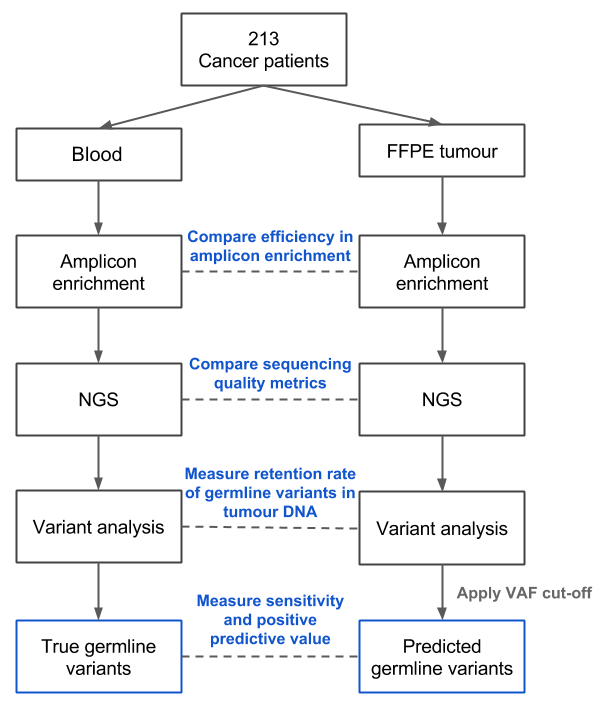
\includegraphics[scale=0.5]{study_design.png}
	\caption{Schematic description of study design and data analyses.}
	\label{fig:study_design}
\end{figure}

%%%%%%%%%%%%%%%%%%%%%%%%%%%%%%%%%%%%%%%%%%%%%%%%%%%%%%%%%%%%%%%%%%%%%
%%%%%%%%%%%%%%%%%%%%%%%%%%%%%%%%%%%%%%%%%%%%%%%%%%%%%%%%%%%%%%%%%%%%%

%%%%%%%%%%%%%%%%%%%%%%%%%%%%%%%%%%%%%%%%%%%%%%%%%%%%%%%%%%%%%%%%%%%%%%
\section{Patient samples}
\label{sec:Patientsamples}

Blood and FFPE tumour samples were acquired from 213 patients who provided informed consent for The OncoPanel Pilot (TOP) study (Human Research Ethics Protocol H14­-01212), a pilot study to optimize the OncoPanel, which is an amplicon-based targeted NGS panel for solid tumours. The TOP study also aims to assess the OncoPanel's application for guiding disease management and therapeutic intervention. One blood sample and four FFPE tumours were sequenced in duplicates, which resulted in 217 tumour-normal paired samples (434 sequencing libraries were included in our analyses). Patients in the TOP study are those with advanced cancers including CRC, lung cancer, melanoma, gastrointestinal stromal tumour (\acs{GIST}), and other cancers (\autoref{tbl:cancertypes}). The age of paraffin block for tumour samples ranges from 18 to 5356 days with a median of 274 days.

%%%%%%%%%%%%%%%%%%%%%%%%%%%%%%%%%%%%%%%%%%%%%%%%%%%%%%%%%%%%%%%%%%%%%%
%%%%%%%%%%%%%%%%%%%%%%%%%%%%%%%%%%%%%%%%%%%%%%%%%%%%%%%%%%%%%%%%%%%%%%
\begin{table}[H]
\caption{Distribution of cancer types in the TOP cohort.}
\label{tbl:cancertypes}
\centering
      \begin{tabular}{lccc}
        \hline
        Cancer Type & Number of Cases & Percentage (\%) \\ \hline
        Colorectal & 97 & 46 \\
        Lung & 60 & 28 \\
        Melanoma & 18 & 8 \\
				Other\textsuperscript{$\dagger$} & 16 & 8 \\
				GIST & 7 & 3 \\
				Sarcoma & 4 & 2 \\
				Neuroendocrine & 4 & 2 \\
				Cervical & 2 & 0.9 \\
				Ovarian & 2 & 0.9 \\
				Breast & 2 & 0.9 \\
				Unknown & 1 & 0.5 \\ \hline
      \end{tabular} \\
			\vspace{0.5cm}
\justify
{\small \textsuperscript{$\dagger$}This category includes thyroid, peritoneum, Fallopian tube, gastric, endometrial, squamous cell carcinoma, anal, salivary gland, peritoneal epithelial mesothelioma, adenoid cystic carcinoma, pancreas, breast, gall bladder, parotid epithelial myoepithelial carcinoma, carcinoid, and small bowel cancers.}
\end{table}

%%%%%%%%%%%%%%%%%%%%%%%%%%%%%%%%%%%%%%%%%%%%%%%%%%%%%%%%%%%%%%%%%%%%%%
\section{Sample preparation, library construction, and Illumina sequencing}
\label{sec:Samplepreparation,libraryconstruction,andIlluminasequencing}

Genomic DNA was extracted from blood and FFPE tumour samples using the Gentra Autopure LS DNA preparation platform and QIAamp DNA FFPE tissue kit (Qiagen, Hilden, Germany), respectively. The extracted DNA was sheared according to a previously described protocol \cite{Bosdet2013} to obtain approximate sizes of 3 kb followed by PCR primer merging, amplification of target regions, and adapter ligation using the Thunderstorm NGS Targeted Enrichment System (RainDance Technologies, Lexington, MA) as per manufacturer's protocol. Barcoded amplicons were sequenced with the Illumina MiSeq system for paired end sequencing with a v2 250-bp kit (Illumina, San Diego, CA).

%%%%%%%%%%%%%%%%%%%%%%%%%%%%%%%%%%%%%%%%%%%%%%%%%%%%%%%%%%%%%%%%%%%%%
\newpage
\section{OncoPanel (Amplicon-based targeted sequencing panel for solid tumours)}
\label{sec:OncoPanel}

The OncoPanel assesses coding exons and clinically relevant hotpots of 15 cancer-related genes and six PGx genes that can predict risk of developing chemotherapy-induced toxicity. Primers were designed by RainDance Technologies (Lexington, MA) using the GRCh37/hg19 human reference genome to generate 416 amplicons between 56 bp and 288 bp in size, which interrogate $\sim$20 kb of target bases. Complete list of genes and gene reference models for the OncoPanel is presented in \autoref{tbl:genemodel}, whereas OncoPanel target regions and amplicons are presented in \autoref{tbl:amplicons_target_regions}.

\normalsize
\begin{table}[H]
    \caption{Gene reference models for HGVS nomenclature of OncoPanel genes.}
    \label{tbl:genemodel}
    \centering
    \begin{tabular}{llll}
    \hline
    Gene & Protein & Reference Model \\
    \hline
    \multicolumn{3}{l}{\textit{Cancer-related}}
    \\
    AKT1 & Protein kinase B & NM\_001014431.1 \\
    ALK & Anaplastic lymphoma receptor tyrosine kinase & NM\_004304.3 \\
    BRAF & Serine/threonine-protein kinase B-Raf & NM\_004333.4 \\
    EGFR & Epidermal growth factor receptor & NM\_005228.3 \\
    HRAS & GTPase HRas & NM\_005343.2 \\
    MAPK1 & Mitogen-activated protein kinase 1 & NM\_002745.4 \\
    MAP2K1 & Mitogen-activated protein kinase kinase 1 & NM\_002755.3 \\
    MTOR & Serine/threonine-protein kinase mTOR & NM\_004958.3 \\
    NRAS & Neuroblastoma RAS viral oncogene homolog & NM\_002524.3 \\
    PDGFRA & Platelet-derived growth factor receptor alpha & NM\_006206.4 \\
    PIK3CA & Phosphatidylinositol-4,5-bisphosphate 3-kinase catalytic subunit alpha & NM\_006218.2 \\
    PTEN & Phosphatase and tensin homolog & NM\_000314.4 \\
    STAT1 & Signal transducer and activator of transcription 1 & NM\_007315.3 \\
    STAT3 & Signal transducer and activator of transcription 3 & NM\_139276.2 \\
    TP53 & Tumor protein P53 & NM\_000546.5 \\
    \\
    \multicolumn{3}{l}{\textit{Pharmacogenomics}}
    \\
    DPYD & Dihydropyrimidine dehydrogenase & NM\_000110.3 \\
    GSTP1 & Glutathione S-rransferase pi 1 & NM\_000852.3 \\
    MTHFR & Methylenetetrahydrofolate reductase & NM\_005957.4 \\
    TYMP & Thymidine phosphorylase & NM\_001113755.2 \\
    TYMS & Thymidylate synthetase & NM\_001071.2 \\
    UGT1A1 & Uridine diphosphate (UDP)-glucuronosyl transferase 1A1 & NM\_000463.2\\
    \hline
    \end{tabular}
\end{table}


%%%%%%%%%%%%%%%%%%%%%%%%%%%%%%%%%%%%%%%%%%%%%%%%%%%%%%%%%%%%%%%%%%%%%%
\section{Variant calling pipeline}
\label{sec:Variantcallingpipeline}

\subsection{Read alignment and variant calling}

Reads that passed the Illumina Chastity filter were aligned to the hg19 human reference genome using the \acs{BWA} mem algorithm (version 0.5.9) with default parameters, and the alignments were processed and converted to the BAM format using SAMtools (version 0.1.18). The SAMtools \texttt{mpileup} function \texttt{(samtools mpileup -BA -d 500000 -L 500000 -q 1)} was used to generate pileup files for all target bases followed by variant calling with the VarScan2 \texttt{mpileup2cns} (version 2.3.6) function with parameter thresholds of VAF $\geq$ 10\% and Phred-scaled BAQ score $\geq$ 20 \texttt{(--min-var-freq 0.1 --min-avg-qual 20 --strand-filter 0 --p-value 0.01 --output-vcf --variants)}.

Four genomic positions at which the hg19 human reference genome contains potential risk alleles were identified (\autoref{tbl:potential_risk_alleles}). Hence, patients homozygous for these four risk alleles would not be identified by our standard variant calling procedure. For these four genomic sites, our method for variant calling was modified to provide calls for every patient in the cohort. The VarScan2 \texttt{mpileup2cns} function with parameter thresholds of VAF $\geq$ 25\%, VAF to call homozygote $\geq$ 90\%, BAQ score $\geq$ 20, and fraction of variant reads from each strand $\geq$ 0.1 \texttt{(--min-var-freq 0.25 --min-freq-for-hom 0.9 --min-avg-qual 20 --strand-filter 1 \\--p-value 0.01 --output-vcf)} was used. Next, allelic statuses were re-assigned, in which wild type calls were re-assigned as homozygous variants, while homozygous variants were re-assigned as wild type calls. Corrections to the VAFs of these four genomic sites were also made to ensure that the VAFs reflect percentage of reads with the risk alleles.

%%%%%%%%%%%%%%%%%%%%%%%%%%%%%%%%%%%%%%%%%%%%%%%%%%%%%%%%%%%%%%%%%%%%%%
%%%%%%%%%%%%%%%%%%%%%%%%%%%%%%%%%%%%%%%%%%%%%%%%%%%%%%%%%%%%%%%%%%%%%%

\begin{longtable}{p{0.08\linewidth}|p{0.05\linewidth}p{0.1\linewidth}p{0.13\linewidth}p{0.16\linewidth}p{0.2\linewidth}}
    \caption{Potential risk alleles in the hg19 human reference genome within the target regions of the OncoPanel.}
    \label{tbl:potential_risk_alleles}
        \\
        \hline
        Gene & Chr & Pos & Risk Allele & dbSNP ID & HGVS\textsuperscript{*}
				\\
				\hline
        DPYD & chr1 & 98348885 & C & rs1801265 & p.Cys29Arg c.85T$>$C
        \\
        MTOR & chr1 & 11205058 & G & rs386514433; rs1057079 & p.Ala1577Ala c.4731A$>$G
        \\
        & chr1 & 11288758 & C & rs1064261 & p.Asn999Asn c.2997T$>$C
        \\
        TP53 & chr17 & 7579472 & C & rs1042522 & p.Arg72Pro c.215G$>$C
        \\
				\hline
\end{longtable}
\textsuperscript{*}Description of sequence variants according to the HGVS recommendations.

%%%%%%%%%%%%%%%%%%%%%%%%%%%%%%%%%%%%%%%%%%%%%%%%%%%%%%%%%%%%%%%%%%%%%%
%%%%%%%%%%%%%%%%%%%%%%%%%%%%%%%%%%%%%%%%%%%%%%%%%%%%%%%%%%%%%%%%%%%%%%

\subsection{Variant filtering}

Variant calls were filtered using the VarScan2 \texttt{fpfilter} function with fraction of variant reads from each strand $\geq$ 0.1 and default thresholds for other parameters (\autoref{tbl:varscan_fpfilter_parameters}). The VarScan2 \texttt{fpfilter} removed 247 low quality variants. Seventy germline variants in the blood were also excluded from our analysis because these variants in the tumours were filtered by the VarScan2 \texttt{fpfilter}. There were also 16 risk allele calls in tumour samples that did not pass the strand filter, causing the removal of 10 risk allele calls in the blood samples from our evaluation. Overall, a total of 343 calls were excluded by the VarScan2 \texttt{fpfilter} and strand filter. Manual inspection was performed for a subset of variants, including variants detected within primer regions and in PGx genes, using the Intergrative Genomics Viewer (IGV, version 2.3). This resulted in the removal of 500 spurious calls, which stemmed from software bugs, sequencing artifacts, primer masking, and primer artifacts (\autoref{tbl:spurious_calls}). Eleven low coverage calls ($\leq$ 100x) were also excluded from our analysis. Implementation of this filtering pipeline reduced the raw variant output of 5288 calls from 217 paired tumour-blood samples (434 sequencing libraries) to 4434 calls (\autoref{fig:variant_pipeline}B).

%%%%%%%%%%%%%%%%%%%%%%%%%%%%%%%%%%%%%%%%%%%%%%%%%%%%%%%%%%%%%%%%%%%%%%
%%%%%%%%%%%%%%%%%%%%%%%%%%%%%%%%%%%%%%%%%%%%%%%%%%%%%%%%%%%%%%%%%%%%%%

\begin{table}[H]
\caption{Thresholds for parameters of VarScan2 \texttt{fpfilter} used for filtering raw variant output.}
\label{tbl:varscan_fpfilter_parameters}
\centering
      \begin{tabular}{p{0.3\linewidth}p{0.56\linewidth}cp{0.1\linewidth}}
        \hline
        Parameter & Description & Threshold
				\\
				\hline
				\texttt{--min-var-count} & Min number of var-supporting reads & 4
				\\
        \texttt{--min-var-count-lc} & Min number of var-supporting reads when depth below somaticPdepth & 2
        \\
        \texttt{--min-var-freq} & Min variant allele frequency & 0.1
				\\
        \texttt{--max-somatic-p} & Max somatic p-value & 0.05
				\\
        \texttt{--max-somatic-p-depth} & Depth required to test max somatic p-value & 10
				\\
        \texttt{--min-ref-readpos} & Min average read position of ref-supporting reads & 0.1
				\\
        \texttt{--min-var-readpos} & Min average read position of var-supporting reads & 0.1
				\\
        \texttt{--min-ref-dist3} & Min average distance to effective 3' end of ref reads & 0.1
				\\
        \texttt{--min-var-dist3} & Min average distance to effective 3' end of variant reads & 0.1
				\\
        \texttt{--min-strandedness} & Min fraction of variant reads from each strand & 0.1
				\\
        \texttt{--min-strand-reads} & Min allele depth required to perform the strand tests & 5
				\\
        \texttt{--min-ref-basequal} & Min average base quality for ref allele & 15
				\\
        \texttt{--min-var-basequal} & Min average base quality for var allele & 15
				\\
        \texttt{--min-ref-avgrl} & Min average trimmed read length for ref allele & 90
				\\
        \texttt{--min-var-avgrl} & Min average trimmed read length for var allele & 90
        \\
        \texttt{--max-rl-diff} & Max average relative read length difference (ref - var) & 0.25
        \\
        \texttt{--max-ref-mmqs} & Max mismatch quality sum of ref-supporting reads & 100
        \\
        \texttt{--max-var-mmqs} & Max mismatch quality sum of var-supporting reads & 100
        \\
        \texttt{--max-mmqs-diff} & Max average mismatch quality sum (var - ref) & 50
        \\
        \texttt{--min-ref-mapqual} & Min average mapping quality for ref allele & 15
        \\
        \texttt{--min-var-mapqual} & Min average mapping quality for var allele & 15
        \\
        \texttt{--max-mapqual-diff} & Max average mapping quality (ref - var) & 50
        \\
				\hline
      \end{tabular}
\end{table}

%%%%%%%%%%%%%%%%%%%%%%%%%%%%%%%%%%%%%%%%%%%%%%%%%%%%%%%%%%%%%%%%%%%%%%
%%%%%%%%%%%%%%%%%%%%%%%%%%%%%%%%%%%%%%%%%%%%%%%%%%%%%%%%%%%%%%%%%%%%%%

\subsection{Variant annotation and interpretation}

SnpEff (version 4.2) was used for effect prediction, and the SnpSift package in SnpEff was used to annotate variants with databases such as dbSNP (b138), COSMIC (version 70), 1000 Genomes Project, and \acs{ExAC} (release 0.3) for interpretation. Clinical significance reported by the ClinVar database and literature review were also used for variant interpretation.

%%%%%%%%%%%%%%%%%%%%%%%%%%%%%%%%%%%%%%%%%%%%%%%%%%%%%%%%%%%%%%%%%%%%%%
%%%%%%%%%%%%%%%%%%%%%%%%%%%%%%%%%%%%%%%%%%%%%%%%%%%%%%%%%%%%%%%%%%%%%%

\newpage
\begin{longtable}{p{0.08\linewidth}p{0.05\linewidth}p{0.1\linewidth}p{0.04\linewidth}p{0.04\linewidth}p{0.6\linewidth}}
    \caption{Spurious variants removed by the variant filtering pipeline.}
    \label{tbl:spurious_calls}
        \\
        \hline
        Gene & Chr & Pos & Ref & Alt & Reason
				\\
				\hline
				KIT & chr4 & 55599268 & C & T & Variant masked by primer in FFPE specimen
				\\
        MAPK1 & chr22 & 22162126 & A & G & Variant masked by primer in FFPE specimen
        \\
        MTOR & chr1 & 11186783 & G & A & Sequencing artifact within primer region
        \\
        MTOR & chr1 & 11190646 & G & A & Variant masked by primer in FFPE specimen
        \\
        TYMP & chr22 & 50964446 & A & T & Poor target region, alignment of different sized amplicons
        \\
        TYMP & chr22 & 50964862 & A & T & Poor target region, alignment of different sized amplicons
        \\
        TYMS & chr18 & 673449 & G & C & VarScan2 bug after chr18:673443 c.*447\_*452delTTAAAG
        \\
        UGT1A1 & chr2 & 234668879 & CAT & C & Sequencing artifact at AT repeats in promoter
        \\
        UGT1A1 & chr2 & 234668881 & T & TAC & VarScan2 bug after AT insertion in promoter
        \\
				\hline
\end{longtable}

%%%%%%%%%%%%%%%%%%%%%%%%%%%%%%%%%%%%%%%%%%%%%%%%%%%%%%%%%%%%%%%%%%%%%%
%%%%%%%%%%%%%%%%%%%%%%%%%%%%%%%%%%%%%%%%%%%%%%%%%%%%%%%%%%%%%%%%%%%%%%

\begin{figure}[H]
\centering
	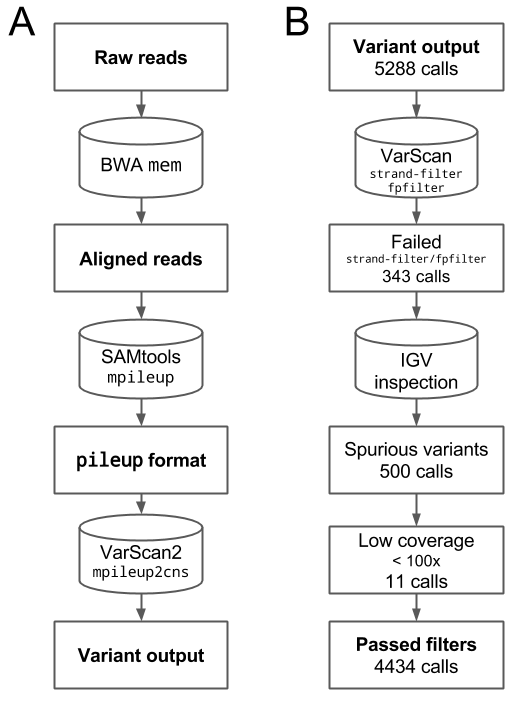
\includegraphics[scale=0.55]{variant_pipeline3.png}
	\caption{Pipelines for (A) variant calling and (B) filtering.}
	\label{fig:variant_pipeline}
\end{figure}

%%%%%%%%%%%%%%%%%%%%%%%%%%%%%%%%%%%%%%%%%%%%%%%%%%%%%%%%%%%%%%%%%%%%%%
\newpage
\section{Sequence analysis}
\label{sec:Sequenceanalysis}

A custom Python script was used to process BAM files to quantify the number of on-target aligned (reads that map to target regions), off-target aligned (reads that map to hg19 but not target regions), and unaligned reads with a Phred-scaled mapping quality (\acs{MAPQ}) score $\geq$ 10. Unaligned reads were also screened against microbial sequences, including viruses, archaea, bacteria, and fungi, to ensure that samples do not contain significant amount of microbial contaminants. Coverage depth for target bases with MAPQ $\geq$ 1 and BAQ $\geq$ 20 was obtained using bam-readcount (https://github.com/genome/bam-readcount). To measure coverage depth of amplicons, the SAMtools \texttt{view} function was used to filter for reads with MAPQ $\geq$ 1 \texttt{(samtools view -b -q 1)} followed by the bedtools \texttt{intersect} function (version 2.25.0) to quantify the number of reads that overlap with amplicon positions \texttt{(intersect -a \$AMPLICON\_POSITIONS -b \$BAM\_FILE -f 0.95 -r -c)}.

Per-base metrics generated using bam-readcount were also used for assessment of sequence artifacts. A custom R script was used to count and categorize the different groups of base changes (i.e. C$>$T/G$>$A, A$>$G/T$>$C, C$>$A/G$>$T, A$>$C/T$>$G, C$>$G/G$>$C, and A$>$T/T$>$A). Unless stated otherwise, analysis of sequence artifacts excludes true variants identified by our VarScan2 variant calling pipeline and base changes with VAF $<$ 1\%, which are considered sequencing errors. All statistical analyses and data visualization were performed using the R statistical software package (version 3.3.2) and associated open-source packages.

%%%%%%%%%%%%%%%%%%%%%%%%%%%%%%%%%%%%%%%%%%%%%%%%%%%%%%%%%%%%%%%%%%%%%%
\section{Application of VAF thresholds to separate germline alterations from somatic mutations}
\label{sec:ApplicationofVAFthresholdstoseparategermlinealterationsfromsomaticmutations}

Variants in the tumours that passed our filtering criteria were subjected to VAF thresholds between 10--45\%. At each VAF cut-off, variants that were not filtered out were considered predicted germline variants. Given that all tumour samples have matched blood samples, true positives were identified as predicted germline variants that overlap with variants in the blood (\autoref{fig:tpfptnfn}). Conversely, false negatives were identified as variants that were filtered out by the VAF cut-off (predicted as somatic), but were present in the blood samples. Sensitivity at each VAF threshold was calculated by dividing the number of true positives with the sum of true positives and false negatives. Because predicted germline variants will be referred to follow-up germline testing, positive predictive values (\acs{PPV}s) were calculated at each VAF cut-off to evaluate precision of our approach. False positives were identified as predicted germline variants that were absent in the blood, and PPV was calculated by dividing the number of true positives with the sum of true positives and false positives.

%%%%%%%%%%%%%%%%%%%%%%%%%%%%%%%%%%%%%%%%%%%%%%%%%%%%%%%%%%%%%%%%%%%%%%
%%%%%%%%%%%%%%%%%%%%%%%%%%%%%%%%%%%%%%%%%%%%%%%%%%%%%%%%%%%%%%%%%%%%%%

\begin{figure}[H]
\centering
	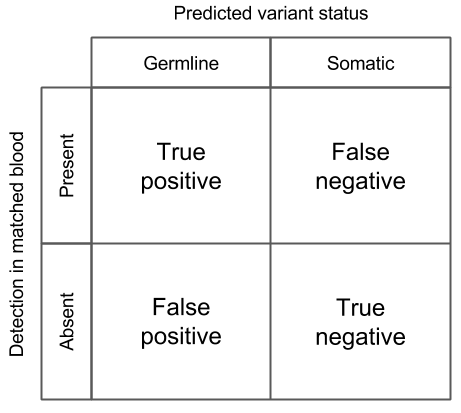
\includegraphics[scale=0.55]{tpfptnfn.png}
	\caption{2x2 contingency table for determination of true positive, false positive, true negative, and false negative variant calls in tumour-only analyses.}
	\label{fig:tpfptnfn}
\end{figure}


%%%%%%%%%%%%%%%%%%%%%%%%%%%%%%%%%%%%%%%%%%%%%%%%%%%%%%%%%%%%%%%%%%%%%%

\endinput


%    3. Characterization of Formalin-Induced DNA Damages
%% The following is a directive for TeXShop to indicate the main file
%%!TEX root = diss.tex

\chapter{Assessment of Formalin-Induced DNA Damage in FFPE Specimens}
\label{ch:AssessmentofFormalin-InducedDNADamageinFFPESpecimens}

Tumour biopsies and resections are often FFPE to preserve cellular morphology for pathological review. The FFPE method also enables storage of tissues at room temperature, minimizing cost and mitigating logistical difficulties in procurement of large archives of clinical specimens \cite{Lou2014}. However, formaldehyde, the main component of formalin, is known to induce DNA damage such as fragmentation and cytosine deamination, which could affect the use of FFPE DNA in clinical genomic testing \cite{Do2015a, Kim2017, Ofner2017, Oh2015, Wong2013, Wong2014, Sikorsky2007}. As DNA derived from blood is one of the gold standards for germline testing, we characterized formalin-induced DNA damage in our data to assess its impact on identification of germline alterations in FFPE DNA. With blood specimens serving as non-formalin-fixed controls, we compared efficiency in amplicon enrichment and sequencing results of FFPE specimens to blood.

%%%%%%%%%%%%%%%%%%%%%%%%%%%%%%%%%%%%%%%%%%%%%%%%%%%%%%%%%%%%%%%%%%%%%
\section{Comparison of efficiency in amplicon enrichment and sequencing results between blood and FFPE specimens}
\label{sec:ComparisonofefficiencyinampliconenrichmentandsequencingresultsbetweenbloodandFFPEspecimens}

%%%%%%%%%%%%%%%%%%%%%%%%%%%%%%%%%%%%%%%%%%%%%%%%%%%%%%%%%%%%%%%%%%%%%

Formalin fixation causes DNA fragmentation that would reduce template DNA for PCR amplification, leading to decreased efficiency in amplicon enrichment methods for FFPE DNA \cite{Didelot2013, Do2015a, Wong2013, Wong2014}. To investigate this effect, we first compared the amplicon yield between blood and FFPE specimens, and a Wilcoxon signed-rank test indicated that amplicon yield in FFPE specimens was significantly lower than blood specimens (\textit{W} = 23613, \textit{Z} = 12.7, \textit{p} = \num{8.3e-62}, \textit{r} = 0.61; \autoref{fig:dna_input_amp_yield}A). However, the amount of DNA input for amplicon enrichment varies across specimens in our study design, and we demonstrated that amplicon yield was weakly correlated with DNA input for both blood and FFPE specimens (Spearman's rank correlation: blood, \textit{r\textsubscript{s}} = 0.29, 95\% CI = 0.16--0.41, \textit{p} = \num{2.1e-5}; FFPE, \textit{r\textsubscript{s}} = 0.25, 95\% CI = 0.12--0.37, \textit{p} = \num{2.5e-4}; \autoref{fig:dna_input_amp_yield}B). To account for the difference in DNA input across specimens, we derived the log\textsubscript{2} fold change between DNA input and amplicon yield (log\textsubscript{2} (Amplicon Yield/DNA Input)) to measure the efficiency in amplicon enrichment. We compared the log\textsubscript{2} fold change in FFPE specimens to blood, and we found a significant decrease in enrichment efficiency in FFPE specimens compared to blood (Wilcoxon signed-rank test, \textit{W} = 24754, \textit{Z} = 12.7, \textit{p} = \num{4.6e-57}, \textit{r} = 0.61; \autoref{fig:dna_input_amp_yield}C). This result implies that production of amplicons is less efficient in FFPE specimens compared to blood, demonstrating the drawback of using FFPE DNA in amplicon-based NGS.

To examine whether blood and FFPE specimens produce comparable sequencing results, we compared read alignments between blood and FFPE specimens. Inspection of on-target aligned reads, which are reads that align to target regions used for variant calling, revealed no significant difference in the percentage of on-target aligned reads between blood and FFPE specimens (Wilcoxon signed-rank test, \textit{W} = \num{10178.5}, \textit{Z} = -1.69, \textit{p} = \num{0.091}, \textit{r} = -0.081; \autoref{fig:alignment_pct}). However, there were more outliers with slightly lower percentage of on-target aligned reads ($<$ 75\%) in FFPE specimens compared to blood, and the distribution of percentage of on-target aligned reads was also wider in FFPE specimens (range: FFPE = 32.5--97.4\%, blood = 74.0--95.9\%), suggesting more variability in the rate of on-target alignment in FFPE specimens than blood. Similarly, no significant difference in the percentage of off-target aligned reads, which are reads that map to the human reference genome but not to target regions, was observed between specimen types (Wilcoxon signed-rank test, \textit{W} = \num{11494.5}, \textit{Z} = -0.359, \textit{p} = \num{0.72}, \textit{r} = -0.017; \autoref{fig:alignment_pct}). Although a Wilcoxon signed-rank test indicated that the percentage of unaligned reads was significantly different between blood and FFPE specimens (\textit{W} = \num{19069}, \textit{Z} = 7.82, \textit{p} = \num{2.4e-16}, \textit{r} = 0.38; \autoref{fig:alignment_pct}), there was only a small decrease in the median percentage of unaligned reads in FFPE specimens compared to blood (median: FFPE = 0.8\%, blood = 1.3\%). Moreover, our data showed no significant difference in percentage of contaminant reads between specimen types (\textit{W} = \num{14877}, \textit{Z} = 3.29, \textit{p} = \num{9.2e-4}, \textit{r} = 0.16; \autoref{fig:alignment_pct}), although there was one extreme outlier in FFPE specimens (range: FFPE = 0.028--64\%, blood = 0.082--8.1\%). While there were minor differences in percentage of unaligned reads between sequencing libraries generated from blood and FFPE DNA, blood and FFPE libraries resulted in comparable percentage of on-target aligned reads, thereby providing equivalent amount of aligned reads for variant calling.

Although blood and FFPE specimens demonstrated no significant difference in the percentage of on-target aligned reads, this result does not reflect the coverage depth of target regions in blood and FFPE specimens. To examine whether discrepancy in coverage depth exists between specimen types, we obtained coverage depth of target bases for all sequencing libraries and normalized per base coverage depth to account for difference in library size. We derived the average per base coverage depth for each library and compared this sequencing metric between blood and FFPE specimens. The average per base coverage depth was significantly different between FFPE and blood specimens (Wilcoxon signed-rank test, \textit{W} = \num{20864}, \textit{Z} = 9.76, \textit{p} = \num{2.5e-26}, \textit{r} = 0.47), but there was only a slight decrease in the average per base coverage depth in FFPE specimens compared to blood (median: FFPE = 1194, blood = 1271). We also calculated the percentages of target bases that met coverage thresholds ranging from zero to 1000x to evaluate coverage uniformity of target bases between blood and FFPE specimens. While coverage uniformity was significantly different between blood and FFPE specimens at coverage levels except at the zero and 100x coverage depth cut-off (Wilcoxon signed-rank test, \textit{p} $<$ \num{0.0001}; \autoref{fig:coverage_stats}), we considered these discrepancies to be technically insignificant because the absolute difference in median percentage of target bases only exceeded 5\% at 500x, 900x, and 1000x coverage thresholds (\autoref{tbl:coverage_uniformity}). Nevertheless, there were more outliers with lower percentage of target bases than median values in FFPE specimens at coverage thresholds between 100x to 1000x, implying that poor coverage uniformity is more profound for a subset of FFPE specimens. Together, our findings reveal that FFPE specimens demonstrated lower efficiency in amplicon enrichment and minor discrepancies in coverage depth and uniformity compared to blood specimens, whereas comparable proportion of on-target read alignments could be attained between specimen types.

%%%%%%%%%%%%%%%%%%%%%%%%%%%%%%%%%%%%%%%%%%%%%%%%%%%%%%%%%%%%%%%%%%%%%
%%%%%%%%%%%%%%%%%%%%%%%%%%%%%%%%%%%%%%%%%%%%%%%%%%%%%%%%%%%%%%%%%%%%%

\begin{figure}[H]
	\centering
	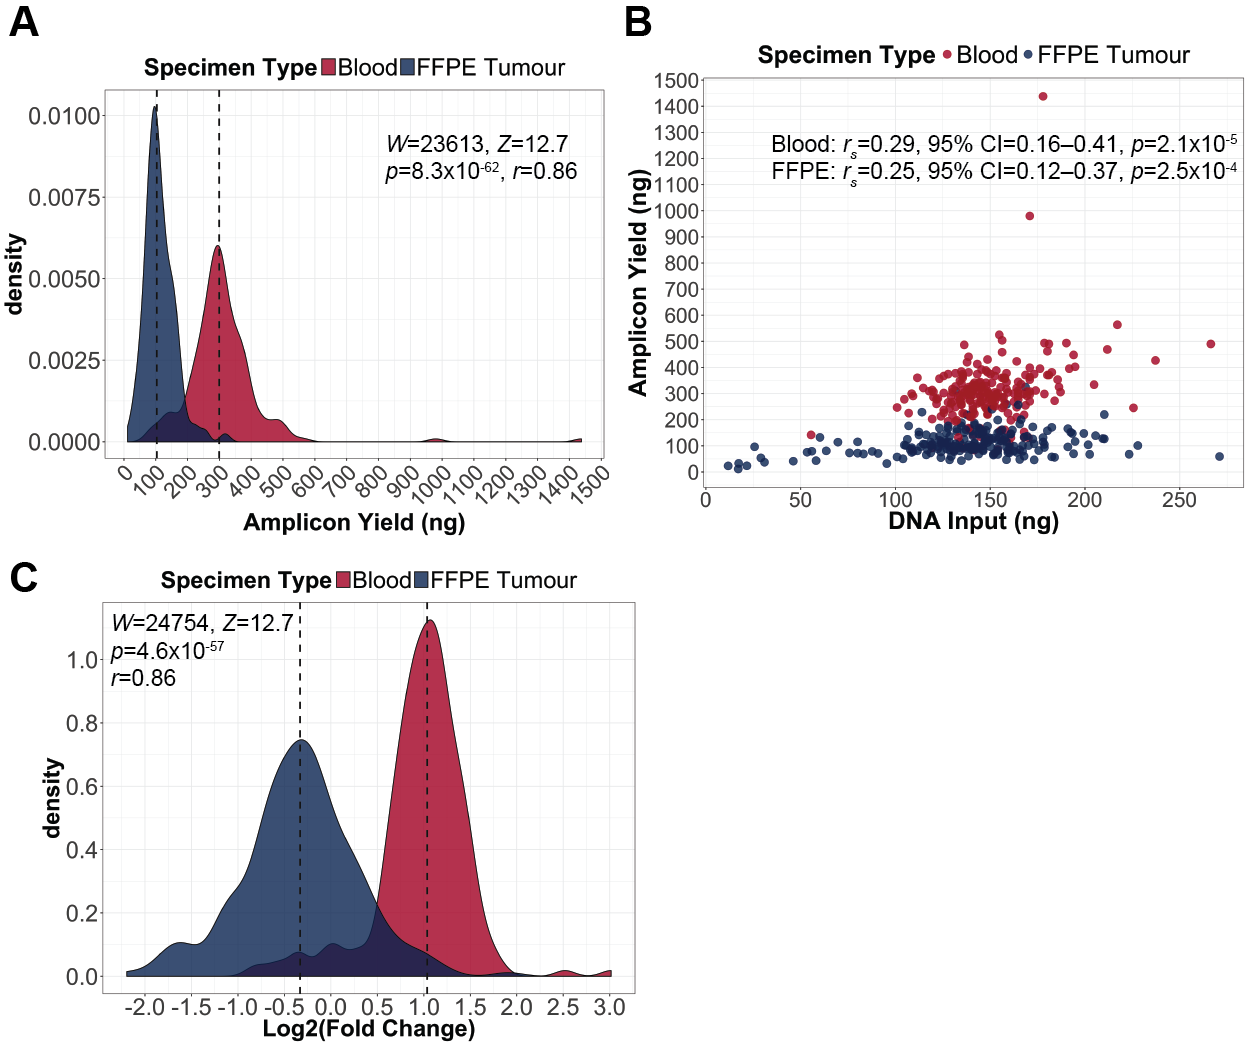
\includegraphics[scale=0.75]{dna_input_amp_yield.png}
	\caption[Comparison of efficiency in amplicon enrichment between blood and FFPE specimens.]{Comparison of efficiency in amplicon enrichment between blood and FFPE specimens. (A) Distributions of amplicon yield in blood and FFPE specimens (Wilcoxon signed-rank test). Dashed lines indicate median amplicon yield in blood and FFPE specimens, which are 299.3 ng and 103.6 ng, respectively. (B) Correlations between amplicon yield and the amount of DNA input for amplicon enrichment in blood and FFPE specimens (Spearman's rank correlation). (C) Distributions of fold change between DNA input and amplicon yield (log\textsubscript{2}), which is used to measure efficiency in amplicon enrichment in blood and FFPE specimens (Wilcoxon signed-rank test). Dashed lines indicate median log\textsubscript{2} fold change in blood and FFPE specimens, which are 1.04 and -0.332, respectively.}
	\label{fig:dna_input_amp_yield}
\end{figure}

%%%%%%%%%%%%%%%%%%%%%%%%%%%%%%%%%%%%%%%%%%%%%%%%%%%%%%%%%%%%%%%%%%%%%
%%%%%%%%%%%%%%%%%%%%%%%%%%%%%%%%%%%%%%%%%%%%%%%%%%%%%%%%%%%%%%%%%%%%%

\begin{figure}[H]
	\centering
	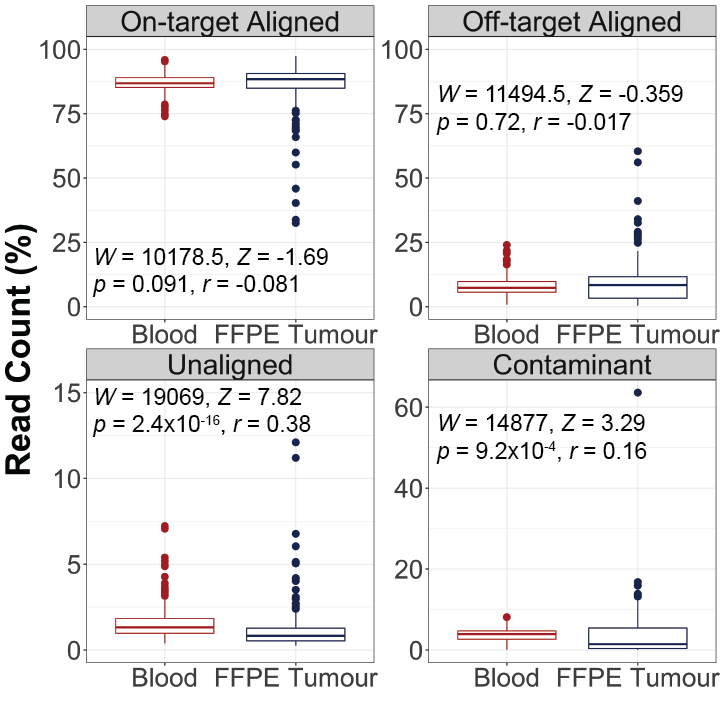
\includegraphics[scale=1]{alignment_pct.png}
	\caption[Assessment of read alignments between blood and FFPE specimens (Wilcoxon signed-rank test).]{Assessment of read alignments between blood and FFPE specimens (Wilcoxon signed-rank test). Box plots show the median (horizontal bar within) and interquartile range (IQR) of percentage of reads, with whiskers representing the range of data not exceeding 1.5x the IQR and circles indicating outliers.}
	\label{fig:alignment_pct}
\end{figure}

%%%%%%%%%%%%%%%%%%%%%%%%%%%%%%%%%%%%%%%%%%%%%%%%%%%%%%%%%%%%%%%%%%%%%
%%%%%%%%%%%%%%%%%%%%%%%%%%%%%%%%%%%%%%%%%%%%%%%%%%%%%%%%%%%%%%%%%%%%%

\begin{figure}[H]
	\centering
	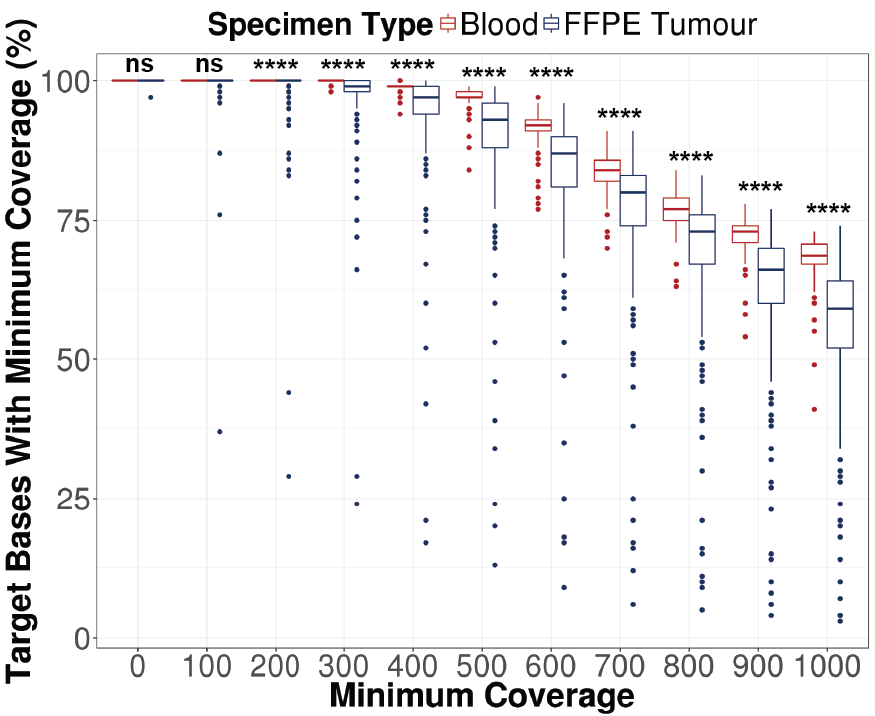
\includegraphics[scale=0.9]{coverage_stats.png}
	\caption[Evaluation of coverage uniformity in blood and FFPE specimens (Wilcoxon signed-rank test, ****\textit{p} $<$ 0.0001, ns = not significant).]{Evaluation of coverage uniformity in blood and FFPE specimens (Wilcoxon signed-rank test, ****\textit{p} $<$ 0.0001, ns = not significant). Per base coverage was normalized to account for difference in library size. Percentage of target bases that met various coverage thresholds was calculated. Box plots show the median (horizontal bar within) and IQR of percentage of target bases that met the respective coverage thresholds, with whiskers representing the range of data not exceeding 1.5x the IQR and circles indicating outliers.}
	\label{fig:coverage_stats}
\end{figure}

%%%%%%%%%%%%%%%%%%%%%%%%%%%%%%%%%%%%%%%%%%%%%%%%%%%%%%%%%%%%%%%%%%%%%
%%%%%%%%%%%%%%%%%%%%%%%%%%%%%%%%%%%%%%%%%%%%%%%%%%%%%%%%%%%%%%%%%%%%%

\begin{table}[H]
\caption{Comparison of coverage uniformity between blood and FFPE specimens using the Wilcoxon signed-rank test.}
\label{tbl:coverage_uniformity}
\centering
      \begin{tabular}{llllllcll}
        \hline
				\multicolumn{1}{l}{ }
				&
				\multicolumn{2}{l}{Blood}
				&&
				\multicolumn{2}{l}{FFPE Tumour}
				&
				\multicolumn{2}{l}{ } \\
				\cline{2-3}\cline{5-6}
        Threshold & Median (\%) & Range (\%) && Median (\%) & Range (\%) & \textit{D}\textsuperscript{$\dagger$} (\%) & \textit{p} ($<$ 0.0001\textsuperscript{*})
				\\
				\hline
				$\geq$ 0x & 100 & 100--100 && 100 & 97.0--100 & 0.0 & 1.0
				\\
				$\geq$ 100x & 100 & 100--100 && 100 & 37.0--100 & 0.0 & \num{2.3e-4}
				\\
				$\geq$ 200x & 100 & 100--100 && 100 & 29.0--100 & 0.0 & \num{2.9e-11}\textsuperscript{*}
				\\
				$\geq$ 300x & 100 & 98.0--100 && 99.0 & 24.0--100 & 1.0 & \num{4.1e-18}\textsuperscript{*}
				\\
				$\geq$ 400x & 99.0 & 94.0--100 && 97.0 & 17.0--100 & 2.0 & \num{5.0e-28}\textsuperscript{*}
				\\
				$\geq$ 500x & 97.0 & 84.0--99.0 && 89.5 & 13.0--99.0 & 7.5 & \num{2.1e-38}\textsuperscript{*}
				\\
				$\geq$ 600x & 92.0 & 77.0--97.0 && 87.0 & 9.0--96.0 & 5.0 & \num{1.5e-32}\textsuperscript{*}
				\\
				$\geq$ 700x & 84.0 & 70.0--91.0 && 80.0 & 6.0--91.0 & 4.0 & \num{5.7e-25}\textsuperscript{*}
				\\
				$\geq$ 800x & 77.0 & 63.0-84.0 && 73.0 & 5.0--83.0 & 4.0 &  \num{4.7e-27}\textsuperscript{*}
				\\
				$\geq$ 900x & 73.0 & 54.0--78.0 && 66.0 & 4.0--77.0 & 7.0 &  \num{4.6e-40}\textsuperscript{*}
				\\
				$\geq$ 1000x & 68.5 & 41.0--73.0 && 59.0 & 3.0-74.0 & 9.5 &  \num{3.6e-42}\textsuperscript{*}
				\\
				\hline
      \end{tabular}
			\justify
			{\small \textsuperscript{$\dagger$}Absolute difference between median of blood and FFPE specimens.}
\end{table}

%%%%%%%%%%%%%%%%%%%%%%%%%%%%%%%%%%%%%%%%%%%%%%%%%%%%%%%%%%%%%%%%%%%%%
\newpage
\section{Reduced coverage depth in FFPE specimens is more pronounced for longer amplicons}
\label{sec:ReducedcoveragedepthinFFPEspecimensismorepronouncedforlongeramplicons}

The OncoPanel consists of 416 amplicons that interrogate coding exons and mutational hotpots of 21 genes, and these amplicons vary in length and GC content. Since we observed discrepancy in sequencing coverage between blood and FFPE specimens, we sought to determine whether this discrepancy is influenced by amplicon length and GC content. We obtained the coverage depth for each amplicon and normalized the coverage depth to account for difference in library size. We found significant differences in coverage depth between blood and FFPE specimens for 336 out of 416 amplicons (Wilcoxon signed-rank test with Benjamini-Hochberg correction, adjusted \textit{p} $<$ 0.0001; \autoref{fig:amp_norm_depth_med_wilcoxon_volcano}). To quantify the amplicon-specific differences in coverage depth, we derived the log\textsubscript{2} fold change in the median coverage depth between blood and FFPE specimens \mbox{(log\textsubscript{2} (Median Coverage\textsubscript{FFPE}/Median Coverage\textsubscript{Blood}))} for each amplicon. Hence, a negative fold change indicates lower coverage depth of the amplicon in FFPE specimens relative to blood specimens, whereas a positive fold change indicates higher coverage depth of the amplicon in FFPE specimens relative to blood specimens. The volcano plot showed that 223 out of the 336 amplicons have negative log\textsubscript{2} fold changes, whereas 113 out of the 336 amplicons have positive log\textsubscript{2} fold changes (\autoref{fig:amp_norm_depth_med_wilcoxon_volcano}). These results indicate that there are differences in coverage depth between FFPE and blood specimens for a large proportion of amplicons in the panel, with substantially more amplicons exhibiting lower coverage depth in FFPE specimens than blood specimens.

We subsequently examined the impact of amplicon length and GC content on the amplicon-specific differences in coverage depth between specimen types, which we measured as the log\textsubscript{2} fold change in median coverage depth between blood and FFPE specimens. We first confirmed that no significant correlation exists between amplicon GC content and length (Pearson's correlation, \textit{r} = 0.045, 95\% CI = -0.051--0.14, \textit{p} = 0.36; \autoref{fig:amp_gc_length}). We then evaluated the correlation between log\textsubscript{2} fold change in amplicon coverage depth and amplicon length, and Pearson's correlation demonstrated a strong, negative correlation between the two variables (\textit{r} = -0.77, 95\% CI = -0.81-- -0.73, \textit{p} = \num{1.4e-82}; \autoref{fig:amp_cov_lm_len_gc}A). This result indicates that coverage depth in FFPE specimens tend to be lower relative to blood specimens as amplicon length increases. On the other hand, coverage depth tend to be enriched in FFPE specimens relative to blood for shorter amplicons. We also assessed the correlation between log\textsubscript{2} fold change in amplicon coverage depth and amplicon GC content, and Pearson's correlation demonstrated a weak, negative correlation between the two variables (\textit{r} = -0.32, 95\% CI = -0.41-- -0.23, \textit{p} = \num{1.8e-11}; \autoref{fig:amp_cov_lm_len_gc}B). Although the correlation is weak, this finding still implies that coverage depth in FFPE specimens tend to be lower relative to blood specimens as amplicon GC content increases, whereas enriched coverage depth in FFPE specimens with respect to blood was observed for amplicons with lower GC content.

Because amplicon length and GC content demonstrated significant correlations with amplicon-specific differences in coverage depth, we determined which contributing factor has a greater effect. We used a multiple linear regression to predict log\textsubscript{2} fold change in amplicon coverage depth based on amplicon length and GC content (\autoref{tbl:multiple_regression}). A significant equation was found (\textit{F}(2, 413) = 427.6, \textit{p} = \num{2.41e-101}), with an adjusted \textit{R\textsuperscript{2}} of 0.673. Predicted log\textsubscript{2} fold change in amplicon coverage depth between blood and FFPE specimens is equal to $$1.63 - \num{6.97e-3}(\textit{Length}) - \num{1.03e-2}(\textit{GC Content}),$$ in which amplicon length is expressed in base pairs (bp) and GC content is expressed as percentage (\%). Both amplicon length and GC content were significant predictors of log\textsubscript{2} fold change in amplicon coverage depth. Based on the standardized coefficients, we compared the strength of predictors within the model to identify the predictor with a greater effect on the response variable. Our assessment showed that one standard deviation increase in amplicon length would lead to a 0.756 standard deviation decrease in log\textsubscript{2} fold change in amplicon coverage depth, whereas one standard deviation increase in amplicon GC content would lead to a 0.288 standard deviation decrease in log\textsubscript{2} fold change in amplicon coverage depth. This result indicates that amplicon length has a stronger association with amplicon-specific differences in coverage depth between specimen types, which we measured as the log\textsubscript{2} fold change in amplicon coverage depth between blood and FFPE specimens, than GC content. Collectively, these findings reveal the challenge imposed by fragmentation damage in FFPE DNA, which results in shorter template DNA that would not be amenable to PCR amplification of longer amplicons.

%%%%%%%%%%%%%%%%%%%%%%%%%%%%%%%%%%%%%%%%%%%%%%%%%%%%%%%%%%%%%%%%%%%%%
%%%%%%%%%%%%%%%%%%%%%%%%%%%%%%%%%%%%%%%%%%%%%%%%%%%%%%%%%%%%%%%%%%%%%

\begin{figure}[H]
	\centering
	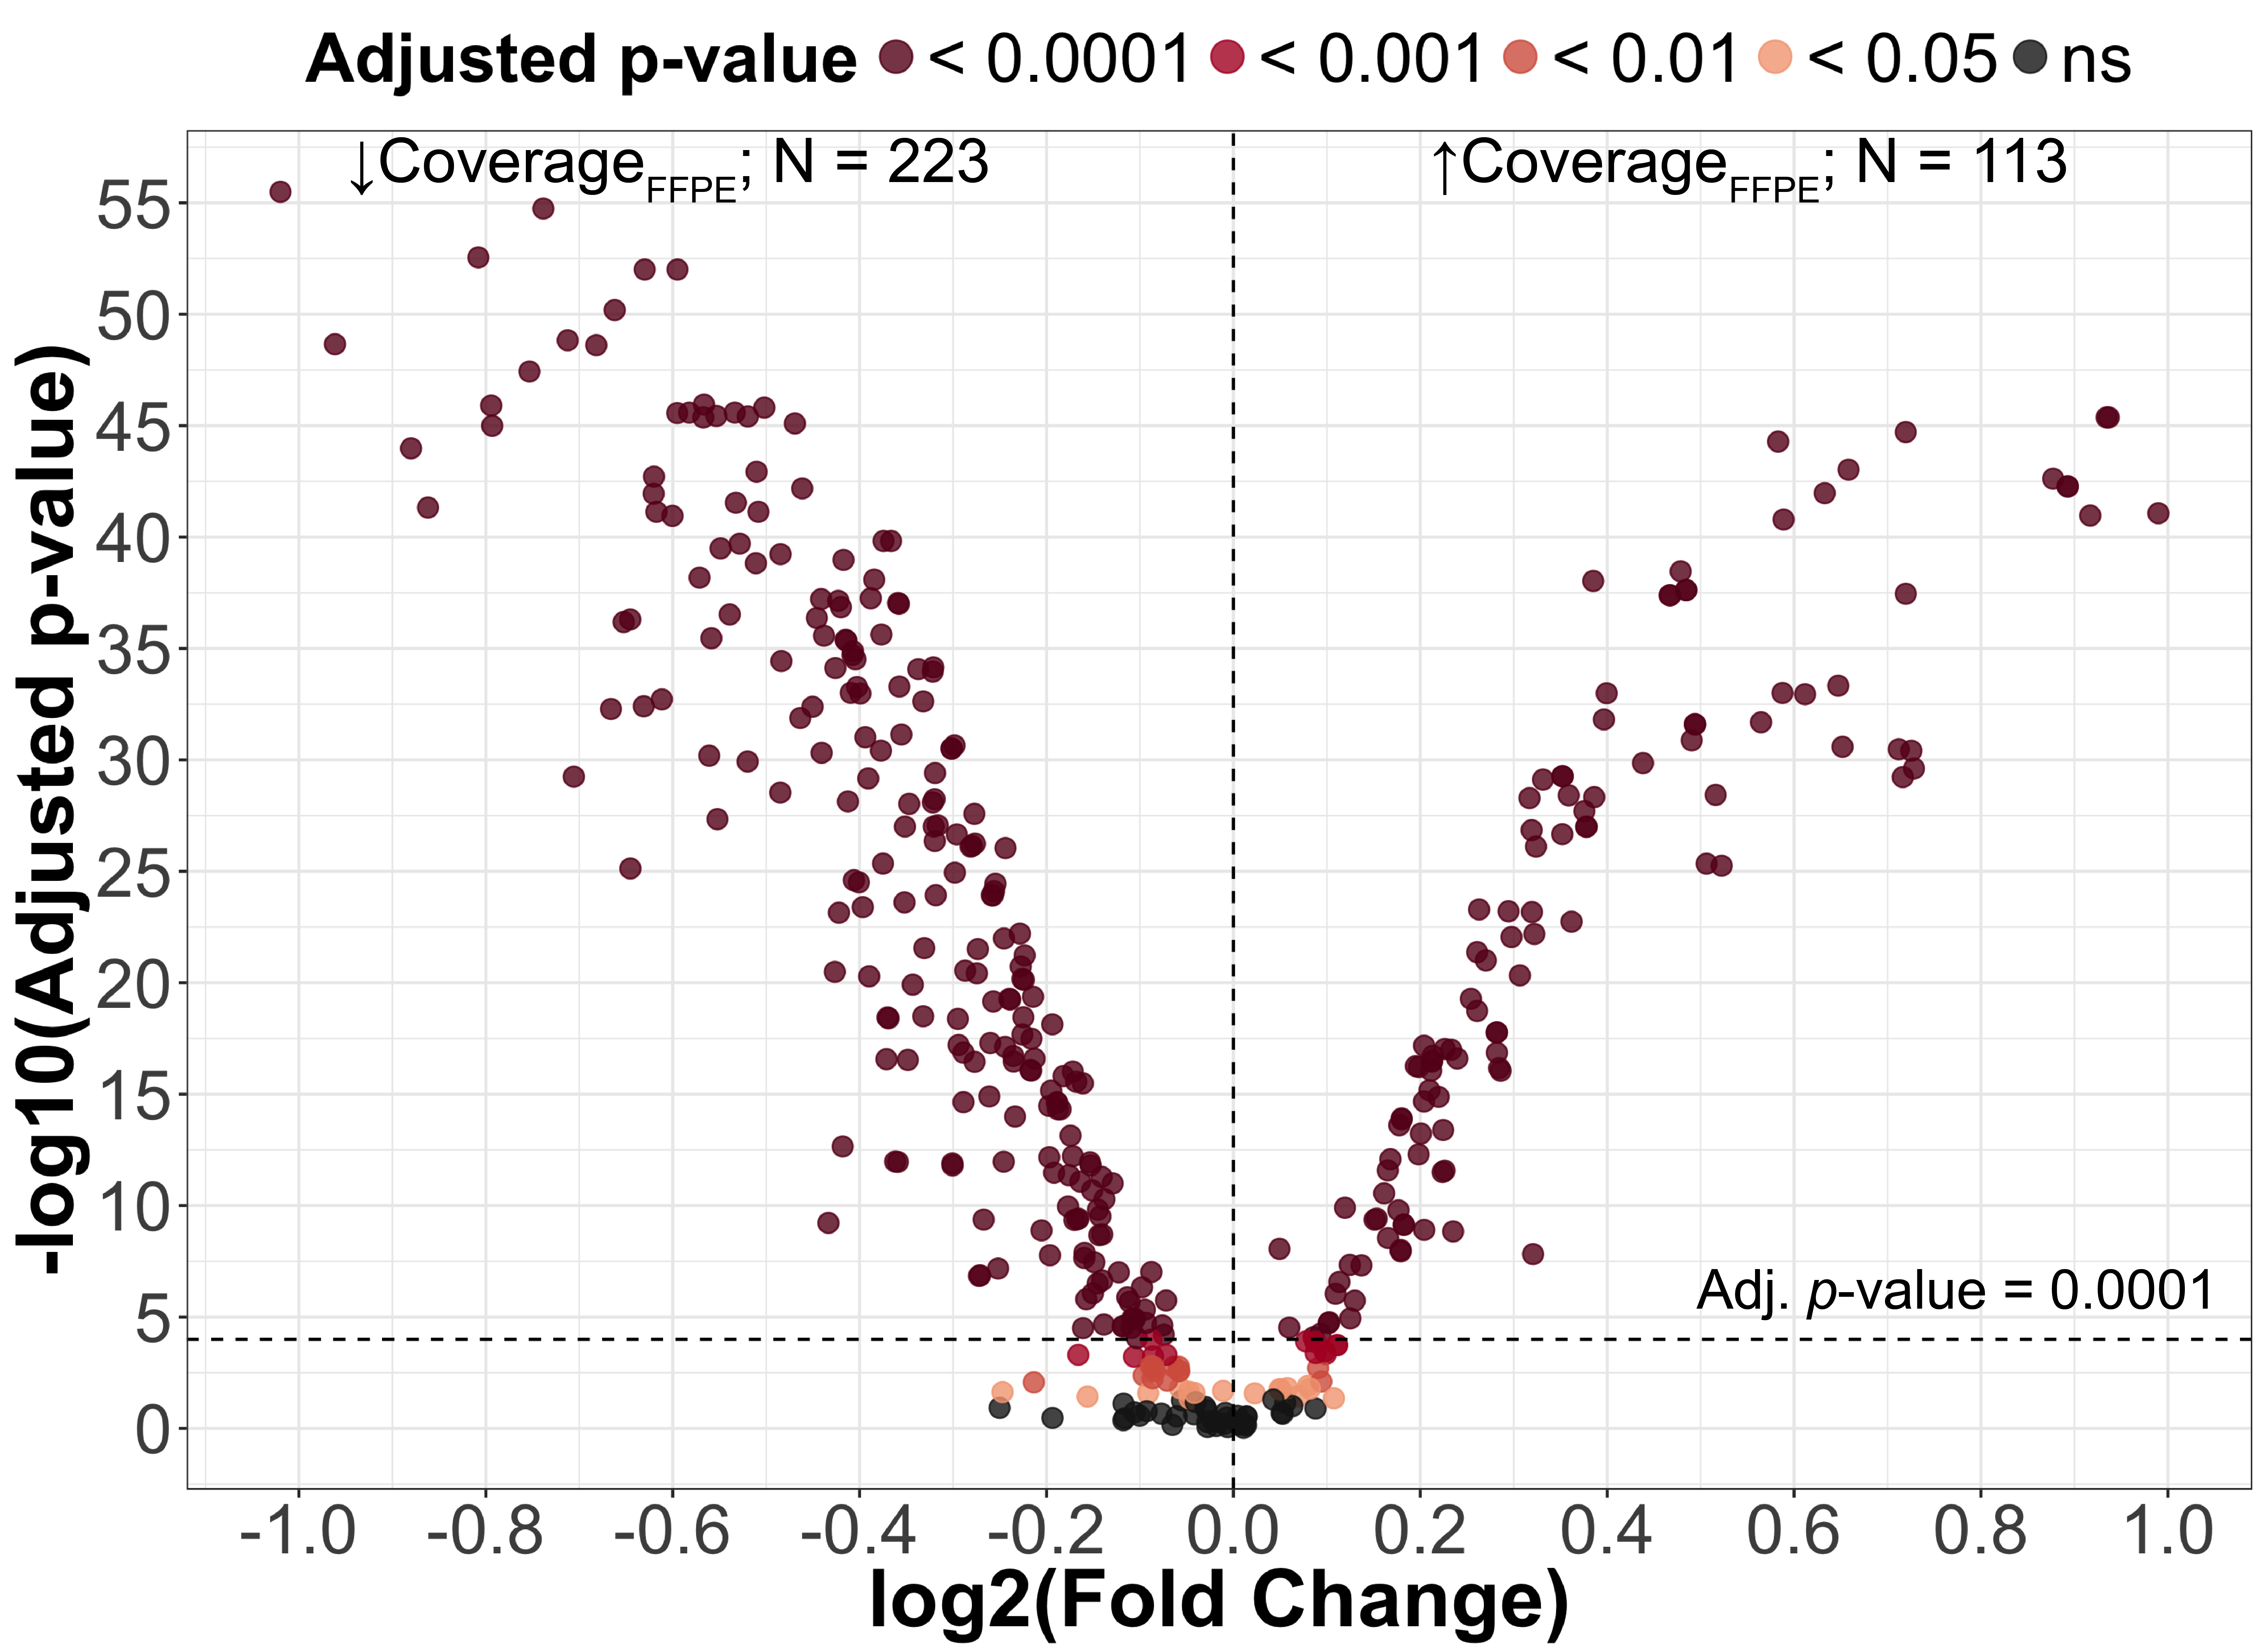
\includegraphics[scale=0.13]{amp_norm_depth_med_wilcoxon_volcano_85.png}
	\caption[Amplicon-specific differences in coverage depth between blood and FFPE specimens.]{Amplicon-specific differences in coverage depth between blood and FFPE specimens. Difference in amplicon coverage depth between specimen types was determined using the Wilcoxon signed-rank test with Benjamini-Hochberg correction (adjusted \textit{p} $<$ 0.0001). Volcano plot illustrates the -log\textsubscript{10} adjusted \textit{p}-value in relation to log\textsubscript{2} fold change between median coverage depth in blood and FFPE specimens (\mbox{log\textsubscript{2} (Median Coverage\textsubscript{FFPE}/Median Coverage\textsubscript{Blood})}) for amplicons in the panel. Negative log\textsubscript{2} fold change indicates lower coverage depth of the amplicon in FFPE specimens relative to blood ($\downarrow \text{Coverage\textsubscript{FFPE}}$), whereas positive log\textsubscript{2} fold change indicates higher coverage depth of the amplicon in FFPE specimens relative to blood ($\uparrow\text{Coverage\textsubscript{FFPE}}$). N = number of amplicons; ns = not significant}
	\label{fig:amp_norm_depth_med_wilcoxon_volcano}
\end{figure}

%%%%%%%%%%%%%%%%%%%%%%%%%%%%%%%%%%%%%%%%%%%%%%%%%%%%%%%%%%%%%%%%%%%%%
%%%%%%%%%%%%%%%%%%%%%%%%%%%%%%%%%%%%%%%%%%%%%%%%%%%%%%%%%%%%%%%%%%%%%

\begin{figure}[H]
	\centering
	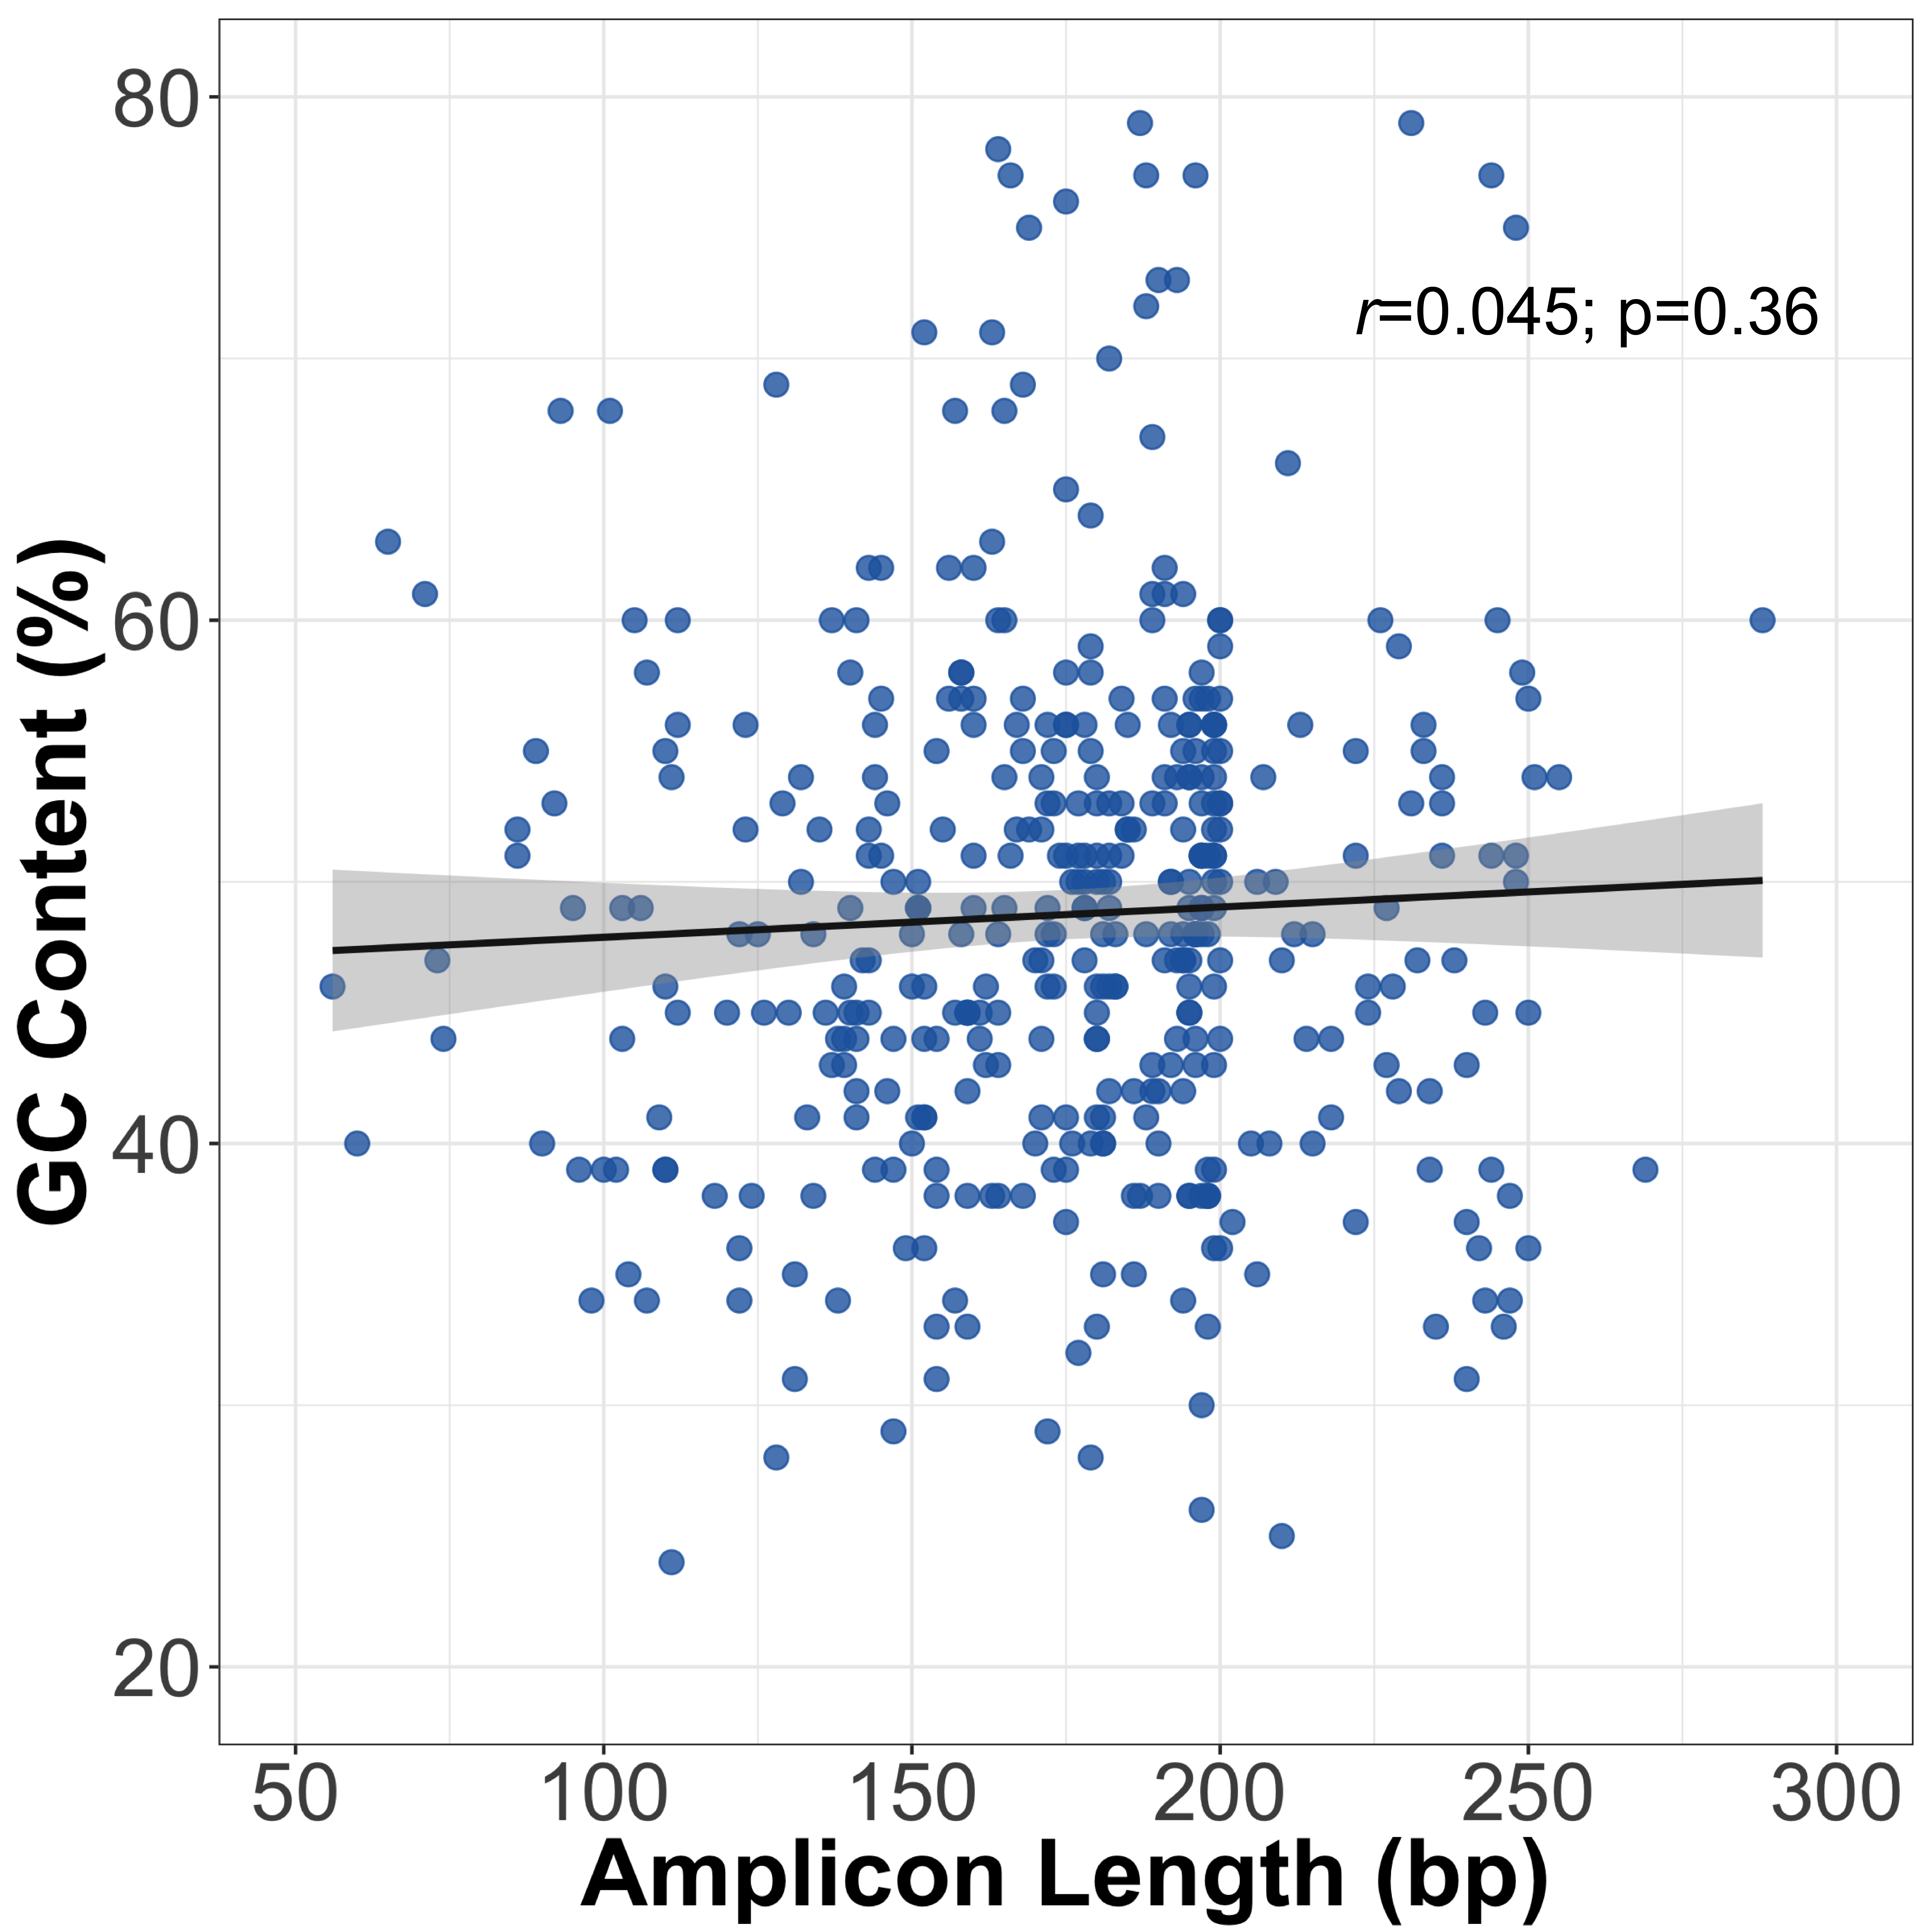
\includegraphics[scale=0.12]{amp_gc_length.png}
	\caption[The relationship between amplicon GC content and amplicon length (Pearson's correlation).]{The relationship between amplicon GC content and amplicon length (Pearson's correlation). Solid line represents the fitted linear relationship between the two variables, and the shaded band indicates pointwise 95\% confidence interval of the fitted linear regression line.}
	\label{fig:amp_gc_length}
\end{figure}

%%%%%%%%%%%%%%%%%%%%%%%%%%%%%%%%%%%%%%%%%%%%%%%%%%%%%%%%%%%%%%%%%%%%%
%%%%%%%%%%%%%%%%%%%%%%%%%%%%%%%%%%%%%%%%%%%%%%%%%%%%%%%%%%%%%%%%%%%%%

\begin{figure}[H]
	\centering
	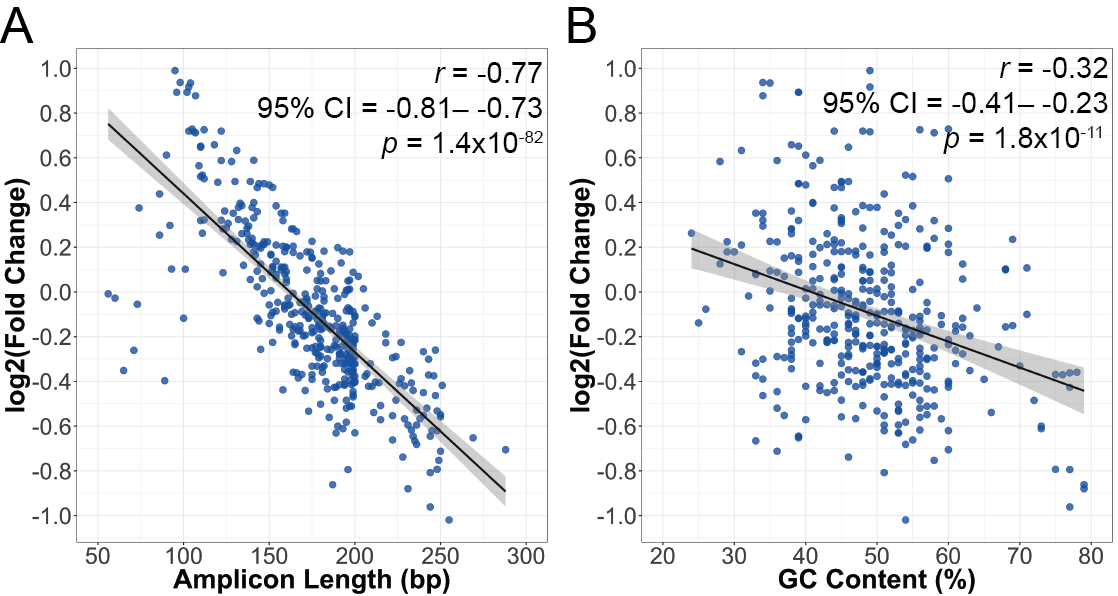
\includegraphics[scale=0.8]{amp_cov_lm_len_gc_85.png}
	\caption[Scatter plots showing log\textsubscript{2} fold change between amplicon coverage depth in blood and FFPE specimens in relation to (A) amplicon length and (B) GC content (Pearson's correlation).]{Scatter plots showing log\textsubscript{2} fold change between amplicon coverage depth in blood and FFPE specimens (\mbox{log\textsubscript{2} (Median Coverage\textsubscript{FFPE}/Median Coverage\textsubscript{Blood})}) in relation to (A) amplicon length and (B) GC content (Pearson's correlation). Solid line represents the fitted linear relationship between the two variables, and the shaded band indicates pointwise 95\% confidence interval of the fitted linear regression line.}
	\label{fig:amp_cov_lm_len_gc}
\end{figure}

%%%%%%%%%%%%%%%%%%%%%%%%%%%%%%%%%%%%%%%%%%%%%%%%%%%%%%%%%%%%%%%%%%%%%
%%%%%%%%%%%%%%%%%%%%%%%%%%%%%%%%%%%%%%%%%%%%%%%%%%%%%%%%%%%%%%%%%%%%%

\begin{table}[H]
\caption[Multiple linear regression to predict log\textsubscript{2} fold change between amplicon coverage depth in blood and FFPE specimens based on amplicon length and GC content.]{Multiple linear regression to predict log\textsubscript{2} fold change between amplicon coverage depth in blood and FFPE specimens (\mbox{log\textsubscript{2} (Median Coverage\textsubscript{FFPE}/Median Coverage\textsubscript{Blood})}) based on amplicon length and GC content.}
\label{tbl:multiple_regression}
\centering
      \begin{tabular}{l|ccccl}
        Variable & Unstandardized Coefficient & Standard Error & Standardized Coefficient & \textit{p}-value
        \\
        \hline
        Length (bp) & \num{-6.97e-3} & \num{2.59e-4} & \num{-7.56e-1} & \num{7.45e-93}
				\\
				GC Content (\%) & \num{-1.03e-2} & \num{1.01e-3} & \num{-2.88e-1} & \num{4.71e-22}
				\\
				\hline
				\\
				 & \multicolumn{4}{r}{Intercept = 1.63, Adjusted R\textsuperscript{2} = 0.673}
				\\
				 & \multicolumn{4}{r}{\textit{F}(2, 413) = 427.6, \textit{p}-value = \num{2.41e-101}}
				\\
				\hline
      \end{tabular} \\
\end{table}

%%%%%%%%%%%%%%%%%%%%%%%%%%%%%%%%%%%%%%%%%%%%%%%%%%%%%%%%%%%%%%%%%%%%%
\newpage
\section{Deamination effects lead to increased C$>$T/G$>$A transitions in FFPE specimens}
\label{sec:DeaminationeffectsleadtoincreasedC$>$T/G$>$AtransitionsinFFPEspecimens}

Formalin fixation not only induces DNA fragmentation, but also base modifications that give rise to sequence artifacts \cite{Do2012, Do2013, Do2015a, Kim2017, Hofreiter2001, Wong2014, Ofner2017, Oh2015}. A prominent type of formalin-induced sequence artifact is C$>$T/G$>$A transitions as a result of deamination of cytosine bases \cite{Do2015a, Kim2017, Wong2014, Oh2015, Lin2014}. To measure the level of formalin-induced artifacts in FFPE specimens, we quantified the fraction of base changes that were not identified as true SNVs by our variant calling pipeline. We only considered high quality bases (BAQ $\geq$ 20) and base changes that were $\geq$ 1\% allele frequency to exclude sequencing errors from our analysis. Base changes were categorized into C$>$T/G$>$A and A$>$G/T$>$C, which are nucleotide transitions, as well as C$>$A/G$>$T, A$>$C/T$>$G, C$>$G/G$>$C, and A$>$T/T$>$A, which are nucleotide transversions. We compared the fraction of base changes between specimen types and found significant differences in fraction of C$>$T/G$>$A and A$>$G/T$>$C between blood and FFPE specimens (Wilcoxon signed rank test, \textit{p} $<$ 0.0001; \autoref{fig:deamination_effect_blood_ffpe}A). As blood DNA is not affected by formalin fixation, we evaluated the prevalence of artifactual base changes in FFPE specimens with respect to blood by calculating the fold change between the median fraction of base changes in blood and FFPE specimens (\autoref{tbl:sum_stats_base_changes}). We noted a substantially higher fold change for C$>$T/G$>$A compared to A$>$G/T$>$C: fraction of C$>$T/G$>$A was 23 times higher in FFPE specimens relative to blood, whereas fraction of A$>$G/T$>$C was 3.1 times higher in FFPE specimens relative to blood. Increased C$>$T/G$>$A artifacts is consistent with cytosine deamination effects that are reportedly predominant in FFPE DNA. On the other hand, A$>$G/T$>$C artifacts could be caused by deamination of adenine to generate hypoxanthine, which forms base pairs with cytosine instead of thymine, changing A-T base pairs to G-C base pairs. Deamination of adenine to hypoxanthine can be catalyzed by an acidic environment \cite{Wang2010}, which can arise in FFPE specimens because formaldehyde can be oxidized to generate formic acid \cite{Do2015a}.

To assess the relative difference in fraction of base changes in FFPE specimens compared to blood specimens, we calculated the log\textsubscript{2} fold change in fraction of base changes between paired blood and FFPE specimens (log\textsubscript{2} (Fraction of Base Changes\textsubscript{FFPE}/Fraction of Base Changes\textsubscript{Blood})). We compared the relative difference in fraction of base changes across different types of base changes, and a Kruskal-Wallis test indicated that type of base changes has a significant effect on the relative difference in fraction of base changes (\textit{H} = 428.5, \textit{p} = \num{2.1e-90}; \autoref{fig:deamination_effect_blood_ffpe_fc}). Multiple pairwise comparison of the relative difference in fraction of base changes was performed using a post-hoc Dunn's test with Benjamini-Hochberg correction. Relative difference in fraction of C$>$T/G$>$A was significantly different compared to the five other types of base changes, and this was similar for A$>$G/T$>$C (adjusted \textit{p} $<$ 0.0001; \autoref{tbl:dunntest}). Although both C$>$T/G$>$A and A$>$G/T$>$C were elevated in FFPE specimens compared to the other base transversions, the magnitude of difference was larger for C$>$T/G$>$A than A$>$G/T$>$C (median log\textsubscript{2} fold change: C$>$T/G$>$A = 4.2, A$>$G/T$>$C = 1.6), which further confirms that deamination of cytosine bases is the most frequent form of sequence artifact in FFPE DNA.

Formalin-induced sequence artifacts often occur at low allele frequency; hence, we examined the prevalence of sequence artifacts at different ranges of allele frequency, including 1--10\%, 10-20\%, and 20-30\%. Because variants were not called within the 1--10\% allele frequency range, we did not remove true SNVs detected by our variant calling pipeline to ensure consistency when comparing fraction of base changes across different ranges of allele frequency. Nevertheless, we adhered to the previous criterion of only including base changes with BAQ $\geq$ 20 in this analysis. For all types of base changes, we noted that the range of allele frequency has a significant effect on fraction of base changes in blood and FFPE specimens (Kruskal-Wallis test, \textit{p} $<$ 0.0001; \autoref{fig:deamination_effect_af_range}), with increased levels of base changes at the 1-10\% allele frequency range compared to 10-20\% and 20-30\%. Because blood DNA represents good quality DNA that is unaffected by formalin fixation, we also compared the fraction of base changes at the 1-10\% allele frequency range in FFPE specimens to blood. Similar to previous analyses, there was a marked increase in C$>$T/G$>$A and a modest increase in A$>$G/T$>$C in FFPE specimens relative to blood within the 1-10\% allele frequency (fold change: C$>$T/G$>$A = 33, A$>$G/T$>$C = 3.1; \autoref{tbl:sum_stats_base_changes_range}). Collectively, our assessment demonstrates that high frequency of C$>$T/G$>$A transitions is present and detectable in FFPE specimens, which indicates that deamination of cytosine is the primary form of formalin-induced sequence artifact, and these artifactual transitions are more prevalent at low, but clinically relevant allele frequency.

%%%%%%%%%%%%%%%%%%%%%%%%%%%%%%%%%%%%%%%%%%%%%%%%%%%%%%%%%%%%%%%%%%%%%
%%%%%%%%%%%%%%%%%%%%%%%%%%%%%%%%%%%%%%%%%%%%%%%%%%%%%%%%%%%%%%%%%%%%%

\begin{figure}[H]
	\centering
	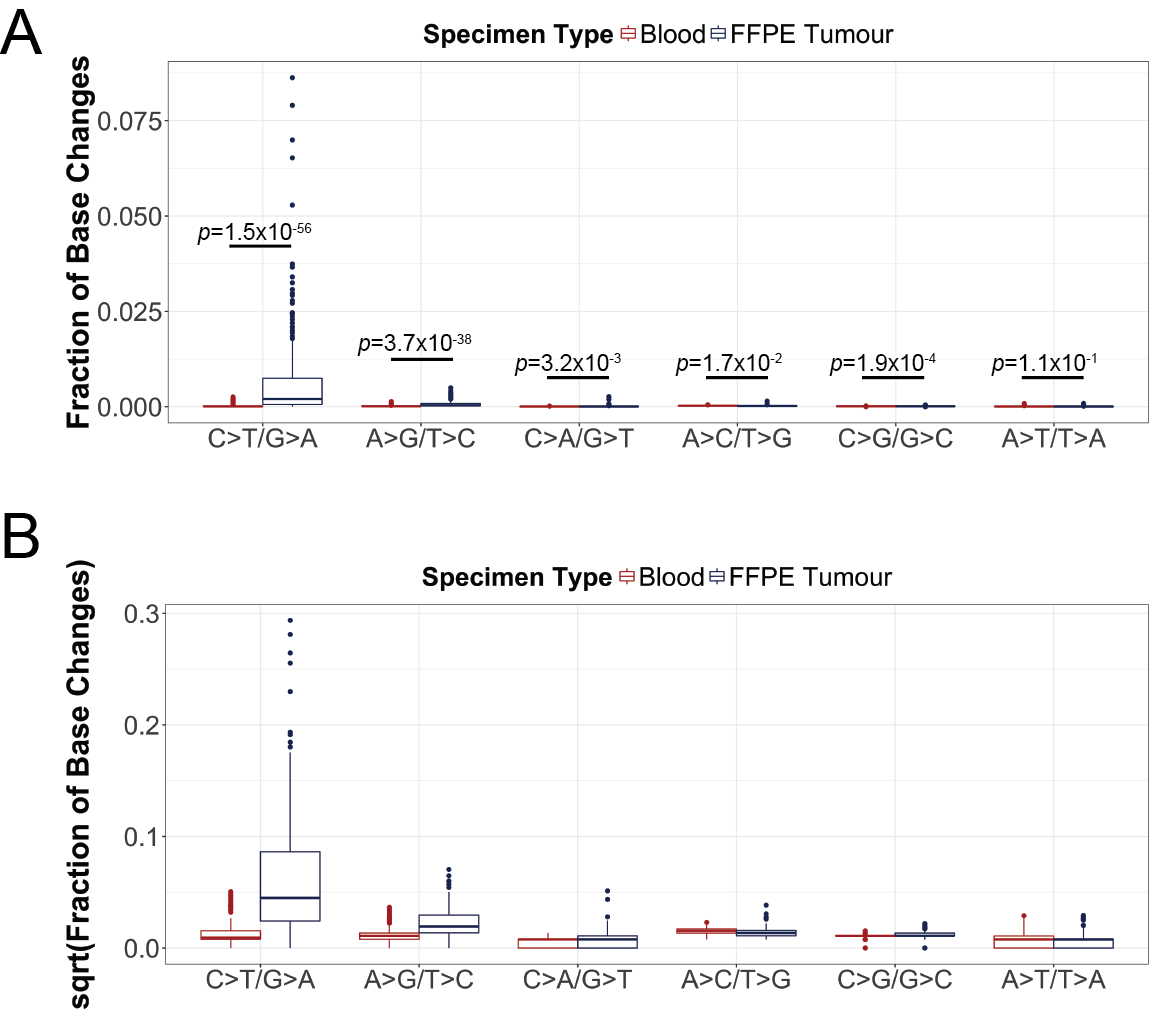
\includegraphics[scale=0.8]{deamination_effect_blood_ffpe.png}
	\caption[Assessment of formalin-induced sequence artifacts in FFPE specimens.]{Assessment of formalin-induced sequence artifacts in FFPE specimens. (A) Comparison of fraction of base changes in blood and FFPE specimens (Wilcoxon signed-rank test). Box plots show the median (horizontal bar within) and IQR of fraction of base changes for different types of base changes, with whiskers representing the range of data not exceeding 1.5x the IQR and circles indicating outliers. (B) Box plots showing square root-transformed fraction of base changes on the Y-axis.}
	\label{fig:deamination_effect_blood_ffpe}
\end{figure}

%%%%%%%%%%%%%%%%%%%%%%%%%%%%%%%%%%%%%%%%%%%%%%%%%%%%%%%%%%%%%%%%%%%%%
%%%%%%%%%%%%%%%%%%%%%%%%%%%%%%%%%%%%%%%%%%%%%%%%%%%%%%%%%%%%%%%%%%%%%

\begin{table}[H]
\caption{Summary statistics of fraction of base changes in blood and FFPE specimens.}
\label{tbl:sum_stats_base_changes}
\centering
      \begin{tabular}{llllllcl}
        \hline
				\multicolumn{1}{l}{ }
				&
				\multicolumn{2}{l}{Blood}
				&&
				\multicolumn{2}{l}{FFPE Tumour}
				&
				\multicolumn{1}{l}{ } \\
				\cline{2-3}\cline{5-6}
        Type of Base Changes & Median & Range && Median & Range & FC\textsuperscript{$\dagger$}
				\\
				\hline
				C$>$T/G$>$A & \num{8.9e-5} & \num{0}--\num{2.6e-3} && \num{2.0e-3} & \num{0}--\num{8.6e-2} & 23
				\\
				A$>$G/T$>$C & \num{1.2e-4} & \num{0}--\num{1.3e-3} && \num{3.7e-4} & \num{0}--\num{5.0e-3} & 3.1
				\\
				C$>$A/G$>$T & \num{6.0e-5} & \num{0}--\num{1.8e-4} && \num{6.0e-5} & \num{0}--\num{2.6e-3} & 1.0
				\\
				A$>$C/T$>$G & \num{2.4e-4} & \num{5.9e-5}--\num{5.3e-4} && \num{1.8e-4} & \num{5.8e-5}--\num{1.4e-3} & 0.77
				\\
				C$>$G/G$>$C & \num{1.2e-4} & \num{0}--\num{2.4e-4} && \num{1.2e-4} & \num{0}--\num{4.8e-4} & 1.0
				\\
				A$>$T/T$>$A & \num{6.0e-5} & \num{0}--\num{8.4e-4} && \num{5.9e-5} & \num{0}--\num{8.6e-4} & 0.99
				\\
				\hline
      \end{tabular}
			\justify
			{\small \textsuperscript{$\dagger$}Fold change (FC) between the median of blood and FFPE specimens.}
\end{table}

%%%%%%%%%%%%%%%%%%%%%%%%%%%%%%%%%%%%%%%%%%%%%%%%%%%%%%%%%%%%%%%%%%%%%
%%%%%%%%%%%%%%%%%%%%%%%%%%%%%%%%%%%%%%%%%%%%%%%%%%%%%%%%%%%%%%%%%%%%%

\begin{figure}[H]
	\centering
	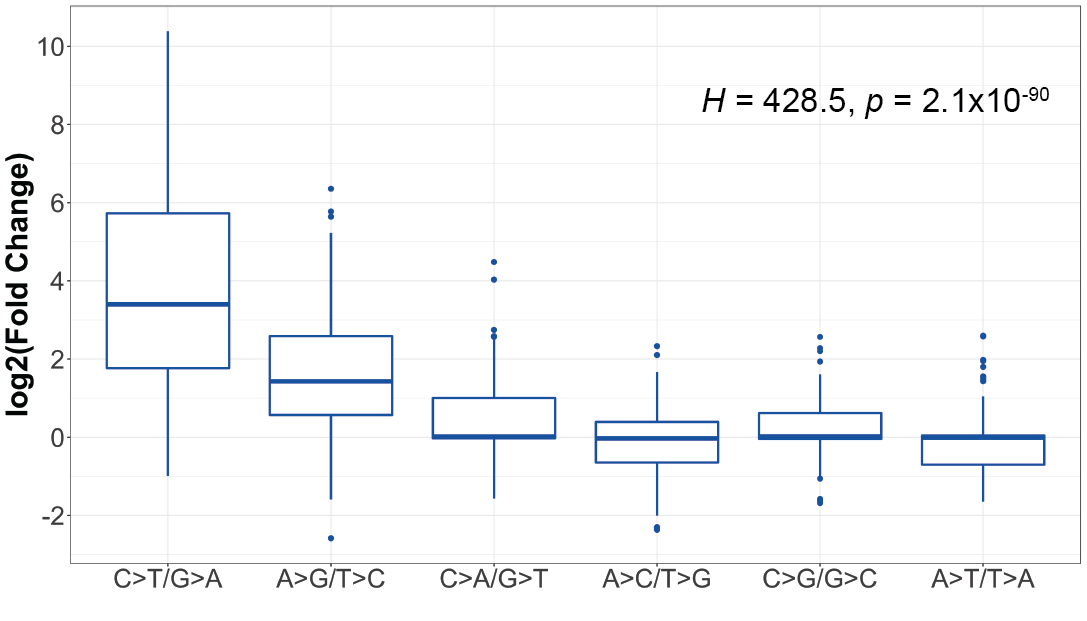
\includegraphics[scale=0.8]{deamination_effect_blood_ffpe_fc.png}
	\caption[Comparison of relative difference in fraction of base changes in FFPE specimens compared to blood (Kruskal-Wallis test).]{Comparison of relative difference in fraction of base changes in FFPE specimens compared to blood (Kruskal-Wallis test). Relative difference was measured as log\textsubscript{2} fold change between fraction of base changes in blood and FFPE specimens \mbox{(log\textsubscript{2} (Fraction of Base Changes\textsubscript{FFPE}/Fraction of Base Changes\textsubscript{Blood}))}. Box plots show the median (horizontal bar within) and IQR of log\textsubscript{2} fold change for different types of base changes, with whiskers representing the range of data not exceeding 1.5x the IQR and circles indicating outliers.}
	\label{fig:deamination_effect_blood_ffpe_fc}
\end{figure}

%%%%%%%%%%%%%%%%%%%%%%%%%%%%%%%%%%%%%%%%%%%%%%%%%%%%%%%%%%%%%%%%%%%%%
%%%%%%%%%%%%%%%%%%%%%%%%%%%%%%%%%%%%%%%%%%%%%%%%%%%%%%%%%%%%%%%%%%%%%

\begin{table}[H]
\caption[Multiple pairwise comparison of log\textsubscript{2} fold change in fraction of base changes between blood and FFPE specimens using Dunn's test with Benjamini-Hochberg multiple hypothesis testing correction.]{Multiple pairwise comparison of log\textsubscript{2} fold change in fraction of base changes between blood and FFPE specimens using Dunn's test with Benjamini-Hochberg multiple hypothesis testing correction. Top values represent Dunn's pairwise \textit{z} statistics, whereas bottom values represent adjusted \textit{p}-value. Asterisk(*) indicates significance level of adjusted \textit{p}-value $<$ 0.0001.}
\label{tbl:dunntest}
\centering
      \begin{tabular}{r|l|l|l|l|ll}
        Type of Base Changes & A$>$C/T$>$G & A$>$G/T$>$C & A$>$T/T$>$A & C$>$A/G$>$T & C$>$G/G$>$C
        \\
        \hline
        A$>$G/T$>$C & -11.7 &  &  &  &
        \\
				 & \num{4.15e-31}\mbox{*} &  &  &  &
				\\
				\hline
        A$>$T/T$>$A & -0.399 & 9.57 &  &  &
        \\
				 & \num{3.45e-1} & \num{1.31e-21}\mbox{*} & & &
				\\
				\hline
        C$>$A/G$>$T & -3.46 & 6.39 & -2.73 &  &
        \\
				 & \num{4.00e-4} & \num{1.52e-10}\mbox{*} & \num{3.99e-3} & &
				\\
				\hline
        C$>$G/G$>$C & -3.02 & 8.63 & -2.17 & 0.918 &
				\\
				 & \num{1.73e-3} & \num{6.76e-18}\mbox{*} & \num{1.71e-2} & \num{1.92e-1} &
        \\
				\hline
        C$>$T/G$>$A & -17.1 & -5.60 & -14.3 & -11.1 & -14.1
        \\
				 & \num{7.78e-65}\mbox{*} & \num{1.76e-8}\mbox{*} & \num{5.10e-46}\mbox{*} & \num{1.32e-28}\mbox{*} & \num{6.46e-45}\mbox{*}
				 \\
				\hline
      \end{tabular} \\
\end{table}

%%%%%%%%%%%%%%%%%%%%%%%%%%%%%%%%%%%%%%%%%%%%%%%%%%%%%%%%%%%%%%%%%%%%%
%%%%%%%%%%%%%%%%%%%%%%%%%%%%%%%%%%%%%%%%%%%%%%%%%%%%%%%%%%%%%%%%%%%%%

\begin{figure}[H]
	\centering
	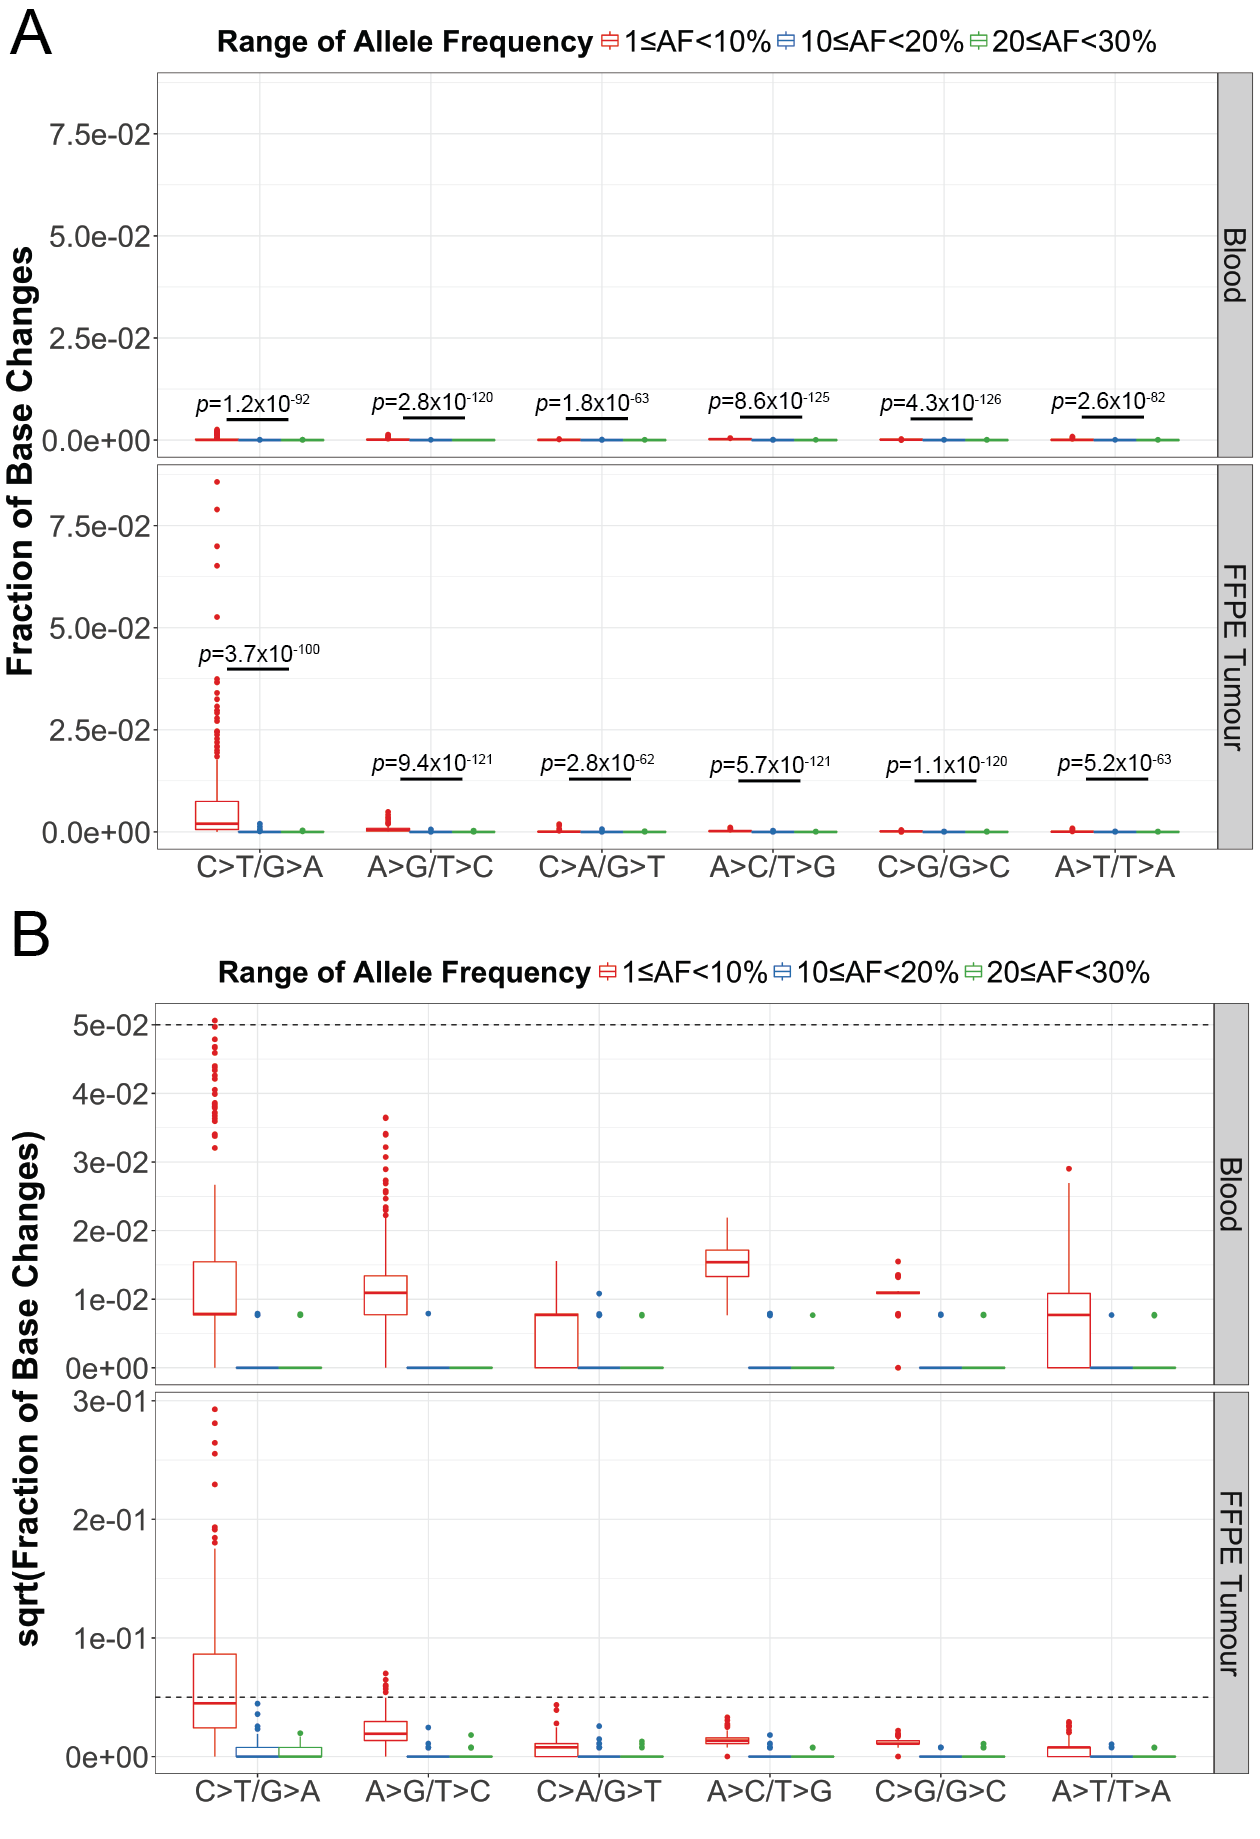
\includegraphics[scale=0.7]{deamination_effect_af_range_2.png}
\end{figure}

%\addtocounter{figure}{-1}
\begin{figure}[H]
  \caption[Assessment of formalin-induced sequence artifacts in FFPE specimens at different ranges of allele frequency.]{Assessment of formalin-induced sequence artifacts in FFPE specimens at different ranges of allele frequency. (A) Comparison of fraction of base changes across different ranges of allele frequency (Kruskal-Wallis test). Box plots show the median (horizontal bar within) and IQR of fraction of base changes for different types of base changes, with whiskers representing the range of data not exceeding 1.5x the IQR and circles indicating outliers. (B) Box plots demonstrating square root-transformed fraction of base changes across different ranges of allele frequency. Dashed lines equal to 0.05 to indicate that the Y-axis scales are different for blood and FFPE tumour plots.}
	\label{fig:deamination_effect_af_range}
\end{figure}

%%%%%%%%%%%%%%%%%%%%%%%%%%%%%%%%%%%%%%%%%%%%%%%%%%%%%%%%%%%%%%%%%%%%%
%%%%%%%%%%%%%%%%%%%%%%%%%%%%%%%%%%%%%%%%%%%%%%%%%%%%%%%%%%%%%%%%%%%%%

\newpage
\begin{table}[H]
\caption{Summary statistics of fraction of base changes in blood and FFPE specimens within 1-10\% allele frequency.}
\label{tbl:sum_stats_base_changes_range}
\centering
      \begin{tabular}{llllllcl}
        \hline
				\multicolumn{1}{l}{ }
				&
				\multicolumn{2}{l}{Blood}
				&&
				\multicolumn{2}{l}{FFPE Tumour}
				&
				\multicolumn{1}{l}{ } \\
				\cline{2-3}\cline{5-6}
        Type of Base Changes & Median & Range && Median & Range & \textsuperscript{$\dagger$}FC
				\\
				\hline
				C$>$T/G$>$A & \num{6.2e-5} & \num{0}--\num{2.6e-3} && \num{2.0e-3} & \num{0}--\num{8.6e-2} & 33
				\\
				A$>$G/T$>$C & \num{1.2e-4} & \num{0}--\num{1.3e-3} && \num{3.7e-4} & \num{0}--\num{4.9e-3} & 3.1
				\\
				C$>$A/G$>$T & \num{6.0e-5} & \num{0}--\num{2.4e-4} && \num{6.0e-5} & \num{0}--\num{1.9e-3} & 1.0
				\\
				A$>$C/T$>$G & \num{2.4e-4} & \num{5.9e-5}--\num{4.8e-4} && \num{1.8e-4} & \num{0}--\num{1.1e-3} & 0.77
				\\
				C$>$G/G$>$C & \num{1.2e-4} & \num{0}--\num{2.4e-4} && \num{1.2e-4} & \num{0}--\num{4.8e-4} & 1.0
				\\
				A$>$T/T$>$A & \num{6.0e-5} & \num{0}--\num{8.4e-4} && \num{5.9e-5} & \num{0}--\num{8.6e-4} & 0.99
				\\
				\hline
      \end{tabular}
			\justify
			{\small \textsuperscript{$\dagger$}Fold change (FC) between the median of blood and FFPE specimens.}
\end{table}


%%%%%%%%%%%%%%%%%%%%%%%%%%%%%%%%%%%%%%%%%%%%%%%%%%%%%%%%%%%%%%%%%%%%%
%%%%%%%%%%%%%%%%%%%%%%%%%%%%%%%%%%%%%%%%%%%%%%%%%%%%%%%%%%%%%%%%%%%%%
\newpage
\section{Increased age of paraffin block results in reduced amplicon yield and elevated level of C$>$T/G$>$A sequence artifacts}
\label{sec:IncreasedageofparaffinblockresultsinpoorerampliconyieldandelevatedeventsofC$>$T/G$>$Asequenceartifacts}

The amount of amplifiable DNA derived from FFPE specimens is dependent on the extent of fragmentation damages. Given two FFPE DNA samples of similar quantity, the sample with more extensive DNA fragmentation would yield reduced amount of PCR amplicons compared to the less fragmented sample \cite{Didelot2013, Wong2014}. Several studies reported increased fragmentation damages in DNA isolated from older paraffin blocks due to longer exposure to environmental conditions \cite{Bass2014, Carrick2015, Ludyga2012, Seiler2016}. As the age of paraffin blocks in our study ranges from 18 to 5356 days, we hypothesized that older paraffin blocks would result in more extensively fragmented DNA, leading to reduced efficiency in amplicon enrichment. Inspection of the relationship between amplicon yield and age of paraffin block demonstrated a moderate, negative correlation (Spearman's rank correlation, \textit{r\textsubscript{s}} = -0.42, 95\% \acs{CI} = -0.52-- -0.30, \textit{p} = \num{1.2e-10}; \autoref{fig:deamination_effect_age_amp_yield}A), suggesting that DNA extraction from older paraffin blocks tend to yield lower amount of amplicons. Because the amount of DNA input for production of amplicons varies across specimens in our study design, a representation of efficiency in amplicon enrichment would be the log\textsubscript{2} fold change between DNA input and amplicon yield. Thus, we assessed the correlation between log\textsubscript{2} fold change and the storage time of FFPE blocks. Similarly, there was a moderate, negative correlation between log\textsubscript{2} fold change and age of paraffin block (Spearman's rank correlation, \textit{r\textsubscript{s}} = -0.42, 95\% CI = -0.53-- -0.30, \textit{p} = \num{1.2e-10}; \autoref{fig:deamination_effect_age_amp_yield}B), implying that production of amplicons is less efficient in FFPE DNA extracted from older paraffin blocks, which is likely caused by more substantial DNA fragmentation.

There are also studies that revealed increased frequency of sequence artifacts in FFPE DNA that are exceedingly fragmented \cite{Carrick2015, Wong2014}. As DNA fragmentation results in reduced template DNA for PCR amplification, this leads to a higher probability for enrichment of sequence artifacts. Our previous evaluation indicated that older paraffin blocks were associated with lower efficiency in amplicon enrichment, which is possibly due to increased fragmentation damages in the extracted DNA. This leads to our hypothesis that older paraffin blocks would yield elevated levels of sequence artifacts, particularly C$>$T/G$>$A transitions, which are the most prominent type of formalin-induced base modifications. To address our hypothesis, we assessed the relationship between fraction of base changes and age of paraffin blocks for different types of base changes (\autoref{fig:deamination_effect_age}). There was a moderate, positive correlation between fraction of C$>$T/G$>$A transitions and age of paraffin block (Spearman's rank correlation, \textit{r\textsubscript{s}} = 0.54, 95\% CI = 0.43--0.63, \textit{p} = \num{1.0e-17}). We also noted a positive correlation between fraction of A$>$G/T$>$C and age of paraffin block (Spearman's rank correlation, \textit{r\textsubscript{s}} = 0.29, 95\% CI = 0.16--0.40, \textit{p} = \num{2.1e-5}), albeit a weak one. As for transversion base changes (i.e. C$>$A/G$>$T, A$>$C/T$>$G, C$>$G/G$>$C, and A$>$T/T$>$A), no significant correlations with age of paraffin block were observed (Spearman's rank correlation, \textit{p} $<$ \num{0.05}). These findings reveal that increased detection of sequence artifacts, especially the common C$>$T/G$>$A changes in FFPE specimens, is associated with long term storage of FFPE blocks.

We subsequently examined how pre-sequencing variables such as age of paraffin block and efficiency in amplicon enrichment correlate with sequencing metrics, which include average per base coverage (normalized to account for library size), percentage of on-target alignments, and fraction of C$>$T/G$>$A changes (\autoref{tbl:spearman_corr}). This assessment would provide insight on how pre-sequencing variables can affect sequencing results, thereby facilitating sample selection if multiple specimens are available before sequencing. We noted a moderate, negative correlation between average per base coverage and age of paraffin block (Spearman's rank correlation, \textit{r\textsubscript{s}} = -0.47, 95\% CI = -0.57-- -0.36, \textit{p} = \num{4.7e-7}), and a weak, negative correlation between percentage of on-target aligned reads and age of paraffin block (Spearman's rank correlation, \textit{r\textsubscript{s}} = -0.35, 95\% CI = -0.46-- -0.23, \textit{p} = \num{8.2e-3}). Conversely, we observed a moderate, positive correlation between average per base coverage and efficiency in amplicon enrichment (Spearman's rank correlation, \textit{r\textsubscript{s}} = 0.52, 95\% CI = 0.42--0.61, \textit{p} = \num{2.3e-11}), and a weak, positive correlation between percentage of on-target aligned reads and efficiency in amplicon enrichment (Spearman's rank correlation, \textit{r\textsubscript{s}} = 0.35, 95\% CI = 0.22--0.45, \textit{p} = \num{2.9e-5}). Since efficiency in amplicon enrichment is inversely correlated with storage time of FFPE blocks, opposing correlations with sequencing metrics were expected for both pre-sequencing variables. Furthermore, there was also a moderate, negative correlation between fraction of C$>$T/G$>$A and efficiency in amplicon enrichment (Spearman's rank correlation, \textit{r\textsubscript{s}} = -0.55, 95\% CI = -0.64-- -0.45, \textit{p} = \num{2.0e-20}). As reduced efficiency in amplicon enrichment is an indicator for low amount of template DNA, the consequent increase in C$>$T/G$>$A changes is the outcome of stochastic enrichment of sequence artifacts. Together, these results reveal that pre-sequencing variables such as age of paraffin block and efficiency in amplicon enrichment could be predictors of sequencing metrics, in which older FFPE blocks are more likely to yield lower efficiency in amplicon enrichment, leading to poorer sequencing results and increased prevalence of artifactual C$>$T/G$>$A transitions.

%%%%%%%%%%%%%%%%%%%%%%%%%%%%%%%%%%%%%%%%%%%%%%%%%%%%%%%%%%%%%%%%%%%%
%%%%%%%%%%%%%%%%%%%%%%%%%%%%%%%%%%%%%%%%%%%%%%%%%%%%%%%%%%%%%%%%%%%%%

\begin{figure}[H]
	\centering
	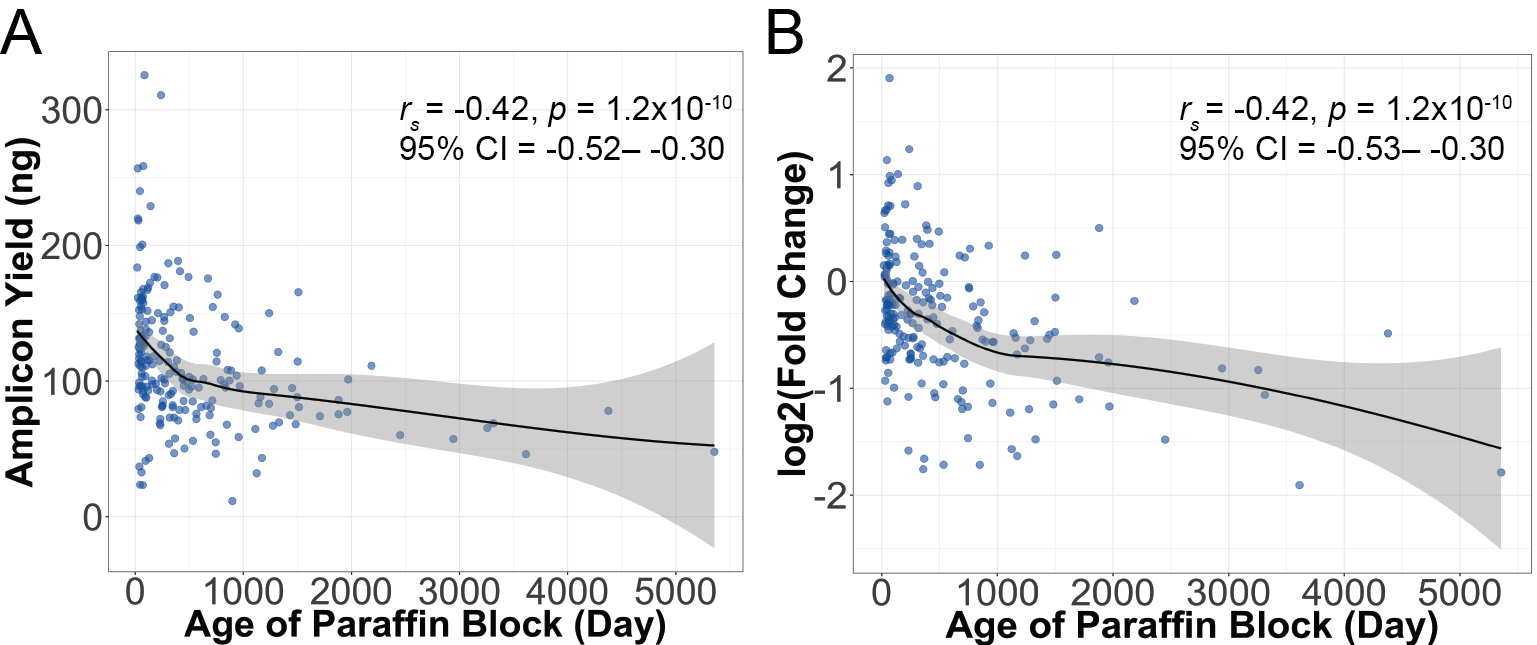
\includegraphics[scale=0.58]{deamination_effect_age_amp_yield.png}
	\caption[Scatter plots showing (A) amplicon yield and (B) efficiency in amplicon enrichment, which is represented by the log\textsubscript{2} fold change between the amount of DNA input for producing amplicons and amplicon yield, in relation to age of paraffin blocks (Spearman's rank correlation).]{Scatter plots showing (A) amplicon yield and (B) efficiency in amplicon enrichment, which is represented by the log\textsubscript{2} fold change between the amount of DNA input for producing amplicons and amplicon yield, in relation to age of paraffin blocks (Spearman's rank correlation). Solid lines represent locally weighted smoothing (LOESS) curves, with shaded bands indicating 95\% confidence interval of the LOESS curves.}
	\label{fig:deamination_effect_age_amp_yield}
\end{figure}

%%%%%%%%%%%%%%%%%%%%%%%%%%%%%%%%%%%%%%%%%%%%%%%%%%%%%%%%%%%%%%%%%%%%
%%%%%%%%%%%%%%%%%%%%%%%%%%%%%%%%%%%%%%%%%%%%%%%%%%%%%%%%%%%%%%%%%%%%%

\begin{figure}[H]
	\centering
	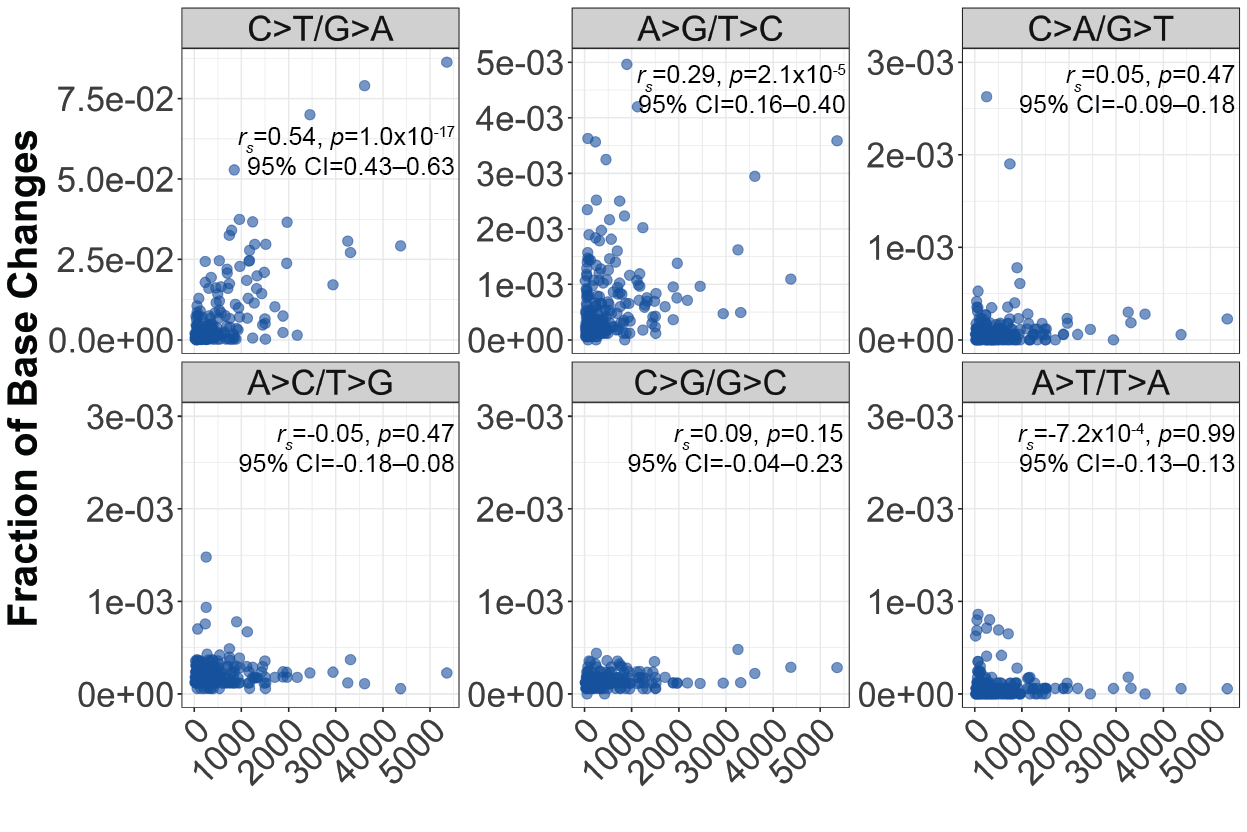
\includegraphics[scale=0.7]{deamination_effect_age.png}
	\caption{The relationship between fraction of base changes and age of paraffin block for different types of base changes (Spearman's rank correlation).}
	\label{fig:deamination_effect_age}
\end{figure}

%%%%%%%%%%%%%%%%%%%%%%%%%%%%%%%%%%%%%%%%%%%%%%%%%%%%%%%%%%%%%%%%%%%%
%%%%%%%%%%%%%%%%%%%%%%%%%%%%%%%%%%%%%%%%%%%%%%%%%%%%%%%%%%%%%%%%%%%%%


\begin{table}[H]
\caption[Spearman's rank correlation between pre-sequencing variables (e.g. enrichment efficiency and age of paraffin block) and sequencing metrics (e.g. fraction of C$>$T/G$>$A, average per base normalized coverage, and on-target aligned reads).]{Spearman's rank correlation between pre-sequencing variables (e.g. enrichment efficiency and age of paraffin block) and sequencing metrics (e.g. fraction of C$>$T/G$>$A, average per base normalized coverage, and on-target aligned reads). Top values represent Spearman's \textit{rho} and 95\% confidence interval in brackets, whereas bottom values represent \textit{p}-value. Asterisk(*) indicates significance level of \textit{p}-value $<$ 0.05.}
\label{tbl:spearman_corr}
\centering
      \begin{tabular}{l|l|l|l|ll}
        Variable & Enrichment & Age of Paraffin & Fraction of & Average Per Base
        \\
				 & Efficiency\textsuperscript{$\dagger$} & Block (Day) & C$>$T/G$>$A & Normalized Coverage
				\\
        \hline
        Age of Paraffin & -0.42 (-0.53-- -0.30) & & &
				\\
				Block (Day) & \num{9.3e-10}\mbox{*} & & &
        \\
				\hline
				Fraction of & -0.55 (-0.64-- -0.45) & 0.54 (0.43--0.63) & &
				\\
				C$>$T/G$>$A & \num{2.0e-20}\mbox{*} & \num{1.0e-17}\mbox{*} & &
				\\
				\hline
				Average Per Base & 0.52 (0.42--0.61) & -0.47 (-0.57-- -0.36) & -0.80 (-0.84-- -0.75) &
				\\
				Normalized Coverage & \num{2.3e-11}\mbox{*} & \num{4.7e-7}\mbox{*} & \num{7.5e-17}\mbox{*} &
				\\
				\hline
				On-target & 0.34 (0.22--0.45) & -0.35 (-0.46-- -0.23) & -0.57 (-0.65-- -0.47) & 0.73 (0.66--0.79)
				\\
				Aligned Reads (\%) & \num{2.9e-5}\mbox{*} & \num{8.2e-3}\mbox{*} & \num{4.2e-8}\mbox{*} & \num{3.1e-58}\mbox{*}
				\\
				\hline
      \end{tabular} \\
			\justify
			{\small \textsuperscript{$\dagger$}log\textsubscript{2} fold change between DNA input for amplicon enrichment and amplicon yield.}
\end{table}


%%%%%%%%%%%%%%%%%%%%%%%%%%%%%%%%%%%%%%%%%%%%%%%%%%%%%%%%%%%%%%%%%%%%%
\endinput
%%%%%%%%%%%%%%%%%%%%%%%%%%%%%%%%%%%%%%%%%%%%%%%%%%%%%%%%%%%%%%%%%%%%%

%%%%%%%%%%%%%%%%%%%%%%%%%%%%%%%%%%%%%%%%%%%%%%%%%%%%%%%%%%%%%%%%%%%%%

\begin{table}[H]
\caption{Assessment of amplicon enrichment results in blood and FFPE specimens. \textit{p} value indicates significance level for Wilcoxon signed-rank test.}
\label{tbl:amplicon_generation}
			\begin{tabular}{lllllll}
				\hline
			 \multicolumn{1}{l}{ }
			 &
			 \multicolumn{2}{l}{Blood}
			 &&
			 \multicolumn{2}{l}{FFPE Tumour}
			 &
			 \multicolumn{1}{l}{ } \\
			 \cline{2-3}\cline{5-6}
			 Parameter & Median & Range && Median & Range & \textit{p} ($<$ 0.05\textsuperscript{*})
			 \\
			 \hline
			 Amplicon Yield (ng) & 299.3 & 84.0--1438.0 && 103.6 & 11.6--325.5 & \num{8.3e-62}\textsuperscript{*}
			 \\
			 DNA Input (ng) & 147.8 & 55.5--266.4 && 140.9 & 11.8--271.0 & \num{3.2e-4}\textsuperscript{*}
			 \\
			 log2(\( \frac{\text{Amplicon Yield}}{\text{DNA Input}} \)) & 1.04 & -0.845--3.01 && -0.332 & -2.20--1.90 & \num{4.6e-57}\textsuperscript{*}
			 \\
			 \hline
			\end{tabular} \\
\end{table}

%%%%%%%%%%%%%%%%%%%%%%%%%%%%%%%%%%%%%%%%%%%%%%%%%%%%%%%%%%%%%%%%%%%%%
%%%%%%%%%%%%%%%%%%%%%%%%%%%%%%%%%%%%%%%%%%%%%%%%%%%%%%%%%%%%%%%%%%%%%

\begin{table}[H]
\caption{Comparison of read alignments between blood and FFPE specimens. \textit{p} value indicates significance level for Wilcoxon signed-rank test.}
\label{tbl:alignment}
      \begin{tabular}{lllllll}
        \hline
				\multicolumn{1}{l}{ }
				&
				\multicolumn{2}{l}{Blood}
				&&
				\multicolumn{2}{l}{FFPE Tumour}
				&
				\multicolumn{1}{l}{ } \\
				\cline{2-3}\cline{5-6}
        Parameter & Median & Range && Median & Range & \textit{p} ($<$ 0.05\textsuperscript{*})
				\\
				\hline
				On-target Aligned Reads (\%) & 86.8 & 74.0--95.9 && 88.4 & 32.5--97.4 & \num{0.091}
				\\
				Off-target Aligned Reads (\%) & 7.3 & 0.8--24.0 && 8.4 & 0.4--60.4 & \num{0.72}
				\\
				Unaligned Reads (\%) & 1.3 & 0.4--7.2 && 0.8 & 0.3--12.1 & \num{2.4e-16}\textsuperscript{*}
				\\
				Contaminant (\%) & 3.9 & 0.1--8.1 && 1.4 & 0.03--63.6 &
				\num{9.2e-4}\textsuperscript{*}
				\\
				\hline
      \end{tabular} \\
\end{table}

%%%%%%%%%%%%%%%%%%%%%%%%%%%%%%%%%%%%%%%%%%%%%%%%%%%%%%%%%%%%%%%%%%%%%
%%%%%%%%%%%%%%%%%%%%%%%%%%%%%%%%%%%%%%%%%%%%%%%%%%%%%%%%%%%%%%%%%%%%%

\begin{table}[H]
\caption{Comparison of coverage uniformity between blood and FFPE specimens using the Wilcoxon signed-rank test.}
\label{tbl:metrics}
\centering
      \begin{tabular}{llllllllll}
        \hline
				\multicolumn{1}{l}{ }
				&
				\multicolumn{2}{l}{Blood}
				&&
				\multicolumn{2}{l}{FFPE Tumour}
				&
				\multicolumn{4}{l}{ } \\
				\cline{2-3}\cline{5-6}
        Threshold & Median (\%) & Range (\%) && Median (\%) & Range (\%) & \textit{W} & \textit{Z} & \textit{p} ($<$ 0.05\textsuperscript{*}) & \textit{r}
				\\
				\hline
				$\geq$ 0x & 100.0 & 100.0--100.0 && 100.0 & 97.0--100.0 & 1 & 1.00 & 1.0 & 0.068
				\\
				$\geq$ 100x & 100.0 & 100.0--100.0 && 100.0 & 37.0--100.0 & 91 & 3.61 & \num{2.3e-4}\textsuperscript{*} & 0.25
				\\
				$\geq$ 200x & 100.0 & 100.0--100.0 && 100.0 & 29.0--100.0 & 666 & 5.99 & \num{2.9e-11}\textsuperscript{*} & 0.41
				\\
				$\geq$ 300x & 100.0 & 98.0--100.0 && 99.0 & 24.0--100.0 & 7696 & 8.17 & \num{4.1e-18}\textsuperscript{*} & 0.55
				\\
				$\geq$ 400x & 99.0 & 94.0--100.0 && 97.0 & 17.0--100.0 & 13934 & 10.0 & \num{5.0e-28}\textsuperscript{*} & 0.68
				\\
				$\geq$ 500x & 97.0 & 84.0--99.0 && 89.5 & 13.0--99.0 & 19880.5 & 11.3 & \num{2.1e-38}\textsuperscript{*} & 0.77
				\\
				$\geq$ 600x & 92.0 & 77.0--97.0 && 87.0 & 9.0--96.0 & 20762 & 10.6 & \num{1.5e-32}\textsuperscript{*} & 0.72
				\\
				$\geq$ 700x & 84.0 & 70.0--91.0 && 80.0 & 6.0--91.0 & 18458.5 & 9.54 & \num{5.7e-25}\textsuperscript{*} & 0.65
				\\
				$\geq$ 800x & 77.0 & 63.0-84.0 && 73.0 & 5.0--83.0 & 18127 & 9.87 & \num{4.7e-27}\textsuperscript{*} & 0.67
				\\
				$\geq$ 900x & 73.0 & 54.0--78.0 && 66.0 & 4.0--77.0 & 20706 & 11.5 & \num{4.6e-40}\textsuperscript{*} & 0.78
				\\
				$\geq$ 1000x & 68.5 & 41.0--73.0 && 59.0 & 3.0-74.0 & 21054.5 & 11.7 & \num{3.6e-42}\textsuperscript{*} & 0.79
				\\
				\hline
      \end{tabular} \\
\end{table}

%%%%%%%%%%%%%%%%%%%%%%%%%%%%%%%%%%%%%%%%%%%%%%%%%%%%%%%%%%%%%%%%%%%%%
% Orphaned text
%%%%%%%%%%%%%%%%%%%%%%%%%%%%%%%%%%%%%%%%%%%%%%%%%%%%%%%%%%%%%%%%%%%%%

The study comprised of 213 patients with FFPE tumour and matched blood specimens that were subjected to evaluation with the OncoPanel, an amplicon-based NGS panel for solid tumours. Sequencing data of tumour-normal paired samples were processed and analyzed with a custom variant calling pipeline.

the median coverage depth of amplicons and amplicon length in both blood and FFPE specimens (\autoref{fig:amp_cov_lm_len}A). While we found no significant correlation between median coverage depth and amplicon length in blood specimens (Pearson's correlation, \textit{r} = 0.042, 95\% CI = -0.054--0.14, \textit{p} = 0.39), we observed a negative correlation in FFPE specimens (Pearson's correlation, \textit{r} = -0.28, 95\% CI = -0.37-- -0.19, \textit{p} = \num{7.4e-9}). We evaluated the relationship between the discrepancy in amplicon coverage depth between FFPE and blood specimens, which was calculated as the log2 fold change from the median coverage depth in blood specimens to the median coverage depth in FFPE specimens (log2\( \frac{\text{Median Coverage Depth in FFPE}}{\text{Median Coverage Depth in Blood}} \)), and amplicon length (\autoref{fig:amp_cov_lm_len}B).

To assess the effect of amplicon GC content on coverage depth of amplicons, we explored the correlation between the median coverage depth of amplicons and amplicon GC content in blood and FFPE specimens (\autoref{fig:amp_cov_lm_gc}A). Using Pearson's correlation, we identified weak, negative correlations between median coverage depth and amplicon GC content in both blood and FFPE specimens (blood: \textit{r} = -0.16, 95\% CI = -0.25-- -0.067, \textit{p} = \num{8.7e-4}; FFPE: \textit{r} = -0.29, 95\% CI = -0.38-- -0.20 \textit{p} = \num{1.0e-9}). We next assessed the relationship between the discrepancy in amplicon coverage depth between FFPE and blood specimens (log2\( \frac{\text{Median Coverage Depth in FFPE}}{\text{Median Coverage Depth in Blood}} \)) and amplicon GC content (\autoref{fig:amp_cov_lm_gc}B). In contrast to the strong, negative correlation observed for the log2 fold change in amplicon coverage depth in relation to amplicon length, Pearson's correlation demonstrated a weak, negative correlation between the log2 fold change in amplicon coverage depth and amplicon GC content (\textit{r} = -0.31, 95\% CI = -0.40-- -0.22, \textit{p} = \num{1.1e-10}). While the correlation is weak, this finding still implies that increased amplicon GC content has a significant impact on the decrease in amplicon coverage depth in FFPE specimens relative to blood specimens.

%%%%%%%%%%%%%%%%%%%%%%%%%%%%%%%%%%%%%%%%%%%%%%%%%%%%%%%%%%%%%%%%%%%%%
%%%%%%%%%%%%%%%%%%%%%%%%%%%%%%%%%%%%%%%%%%%%%%%%%%%%%%%%%%%%%%%%%%%%%

\begin{figure}[H]
	\centering
	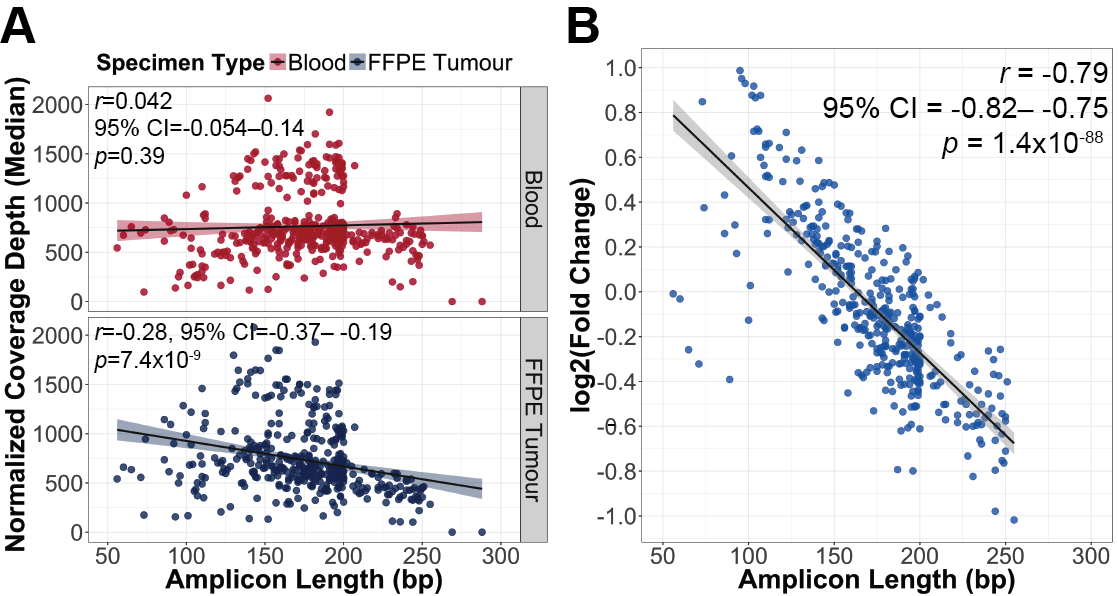
\includegraphics[scale=0.85]{amp_cov_lm_len.png}
	\caption{The effect of amplicon length on coverage depth of amplicons. Coverage depth of amplicons was normalized to account for difference in library size and log2 fold change between the median coverage depth in blood and FFPE specimens (log2\( \frac{\text{Median Coverage Depth in FFPE}}{\text{Median Coverage Depth in Blood}} \)) was calculated for each amplicon. (A) No significant correlation between coverage depth of amplicons and amplicon length was demonstrated in blood specimens, whereas coverage depth of amplicons is negatively correlated with amplicon length in FFPE specimens (Pearson's correlation, \textit{p} $<$ 0.05). (B) Increased in amplicon length leads to lower log2 fold change in amplicon coverage depth between blood and FFPE specimens (Pearson's correlation, \textit{p} $<$ 0.05).}
	\label{fig:amp_cov_lm_len}
\end{figure}

%%%%%%%%%%%%%%%%%%%%%%%%%%%%%%%%%%%%%%%%%%%%%%%%%%%%%%%%%%%%%%%%%%%%%
%%%%%%%%%%%%%%%%%%%%%%%%%%%%%%%%%%%%%%%%%%%%%%%%%%%%%%%%%%%%%%%%%%%%%

\begin{figure}[H]
	\centering
	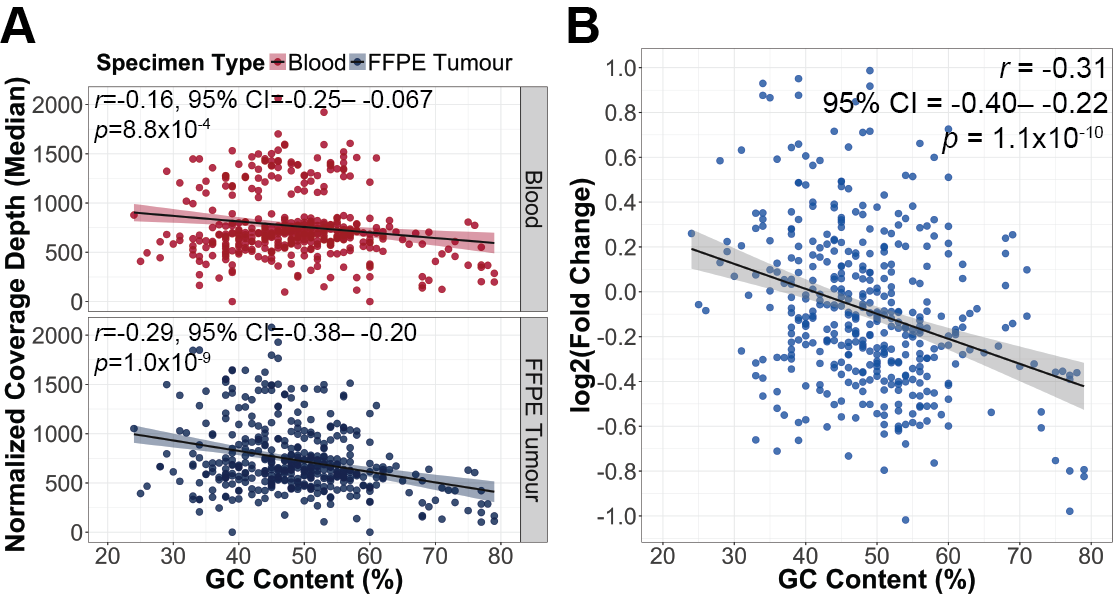
\includegraphics[scale=0.85]{amp_cov_lm_gc.png}
	\caption{The effect of amplicon GC content on coverage depth of amplicons. Coverage depth of amplicons was normalized to account for difference in library size and log2 fold change between the median coverage depth in blood and FFPE specimens (log2\( \frac{\text{Median Coverage Depth in FFPE}}{\text{Median Coverage Depth in Blood}} \)) was calculated for each amplicon. (A) Coverage depth of amplicons is negatively correlated with amplicon GC content in both blood and FFPE specimens (Pearson's correlation, \textit{p} $<$ 0.05). (B) Increased in amplicon GC content leads to lower log2 fold change in amplicon coverage depth between blood and FFPE specimens (Pearson's correlation, \textit{p} $<$ 0.05).}
	\label{fig:amp_cov_lm_gc}
\end{figure}


%    4. Concordance of Germline Pharmacogenomic Variants Between Blood and Tumours
%% The following is a directive for TeXShop to indicate the main file
%%!TEX root = diss.tex

\chapter{Identification of Germline Alterations in FFPE Tumours}
\label{ch:IdentificationofGermlineAlterationsinFFPETumours}

Genomic analyses of tumours can reveal both germline and somatic alterations \cite{Schrader2015, Jones2015a, Meric-Bernstam2016, Bombard2014}. Although simultaneous identification of germline variants could be performed if tumour-normal pairs are sequenced, matched normal samples are not routinely processed in the clinical setting due to logistical difficulties, funding, and time \cite{Frampton2013, Fumagalli2010, Lin2014, Wong2014a}. The TOP study is comprised of 213 patients with tumour and matched blood specimens. This enables us to measure the retention rate of germline alterations in tumour DNA to confirm that tumour DNA is a reliable substrate for identification of germline alterations. We also evaluated the use of VAF threshold to distinguish between germline and somatic statuses of variants identified in tumour DNA. Our goal is to establish a VAF cut-off that could maximize true positive rate for identification of potential germline alterations for referral to downstream germline testing, as well as minimize false positive rate to reduce unnecessary follow-up testing.

%%%%%%%%%%%%%%%%%%%%%%%%%%%%%%%%%%%%%%%%%%%%%%%%%%%%%%%%%%%%%%%%%%%%%
\section{Frequency and interpretation of germline alterations in patients from TOP cohort}
\label{sec:FrequencyandinterpretationofgermlinealterationsinpatientsfromTOPcohort}
%%%%%%%%%%%%%%%%%%%%%%%%%%%%%%%%%%%%%%%%%%%%%%%%%%%%%%%%%%%%%%%%%%%%%

We examined 15 cancer-related genes and six PGx genes in DNA isolated from blood samples from the 213 cancer patients in TOP cohort. We identified a total of 1990 germline alterations that passed our filtering criteria (\autoref{fig:variant_pipeline}B). In 212 out of 213 patients, we detected a total of 1205 variants in the 15 cancer-related genes screened by the OncoPanel, with an average of 5.7 variants per patient (standard error = 0.15, range = 1--11 variants; \autoref{tbl:freq_cancer_genes}). These germline alterations were found at 50 genomic positions and interpreted using various bioinformatics approaches and literature review (\autoref{tbl:germline_cancer_genes}). Through effect prediction using the SnpEff software, we demonstrated that 78\% of these variants were synonymous, 16\% were missense variants, 4\% occurred within splice regions, and 2\% were frameshift variants. Eighteen out of the 50 germline variants were classified as common variants by the 1000 Genomes Project with population frequencies of $\geq$ 1\% in the ExAC database, whereas eight out of the 50 variants were classified as rare variants with population frequencies of $<$ 1\% in the ExAC database.

To assess clinical significance of the 50 germline alterations in cancer-related genes, we used information in the ClinVar database. Our assessment revealed 16\% benign variants, 16\% likely benign variants, 12\% annotated as benign/likely benign, 4\% with conflicting interpretations of pathogenicity, and 2\% with uncertain significance. We were unable to determine the clinical significance of 48\% of the 50 germline variants because these variants were not reported in the ClinVar database. While we found no variants that were pathogenic or likely pathogenic, we identified one \acs{TP53} variant, p.Arg72Pro$/$c.215G$>$C (rs1042522), that is associated with drug response. Based on literature review, clinical studies revealed that the Pro/Pro genotype results in severe neutropenia in ovarian cancer patients receiving cisplatin-based chemotherapy, and poor survival and treatment response in gastric cancer patients receiving paclitaxel and capecitabine combination chemotherapy, as well as 5-fluorouracil-based adjuvant chemotherapy \cite{Khrunin2010, Zha2016, Kim2009, Bojesen2008, Bonafe2004, Huang2008, Yoneda2013, Yang2007, Bougeard2006, Cheng2012, Zhu2007, Zhang2012a}. The combination of evidence from our literature review and the ClinVar database suggests that the \acs{TP53} p.Arg72Pro$/$c.215G$>$C (rs1042522) could be potentially useful in guiding therapeutic intervention for cancer patients.

Furthermore, we identified a total of 785 variants in the six PGx genes screened by the OncoPanel in 212 out of 213 patients, with an average of 3.7 germline alterations per patient (standard error = 0.10, range = 1--8 variants; \autoref{tbl:freq_germline_pgx_genes}). These PGx variants occurred at 23 genomic positions and were interpreted using similar methods to the germline alterations identified in cancer-related genes (\autoref{tbl:germline_pgx_genes}). Effect prediction using the SnpEff software demonstrated that 57\% of these 23 germline variants were missense variants, 17\% were synonymous, 9\% occurred within splice regions, 9\% occurred upstream of a gene, 4\% were located at splice donor sites, and 4\% were present at the 3' untranslated region. Ten out of the 23 germline variants were classified as common variants by the 1000 Genomes Project with population frequencies of $\geq$ 1\% in the ExAC database, whereas one out of the 23 variants was classified as a rare variant with population frequency of $<$ 1\% in the ExAC database.

We also assessed clinical significance of the germline alterations in the PGx genes using the ClinVar database. This assessment demonstrated that 21\% of the 23 variants were categorized as either benign or likely benign, 17\% with conflicting interpretations of pathogenicity, 9\% submitted without assessment of clinical significance, and 4\% with uncertain significance. There was also 17\% of variants that were not reported in the ClinVar database. Although our analysis showed no variants that were pathogenic or likely pathogenic in the PGx genes, we identified seven out of the 23 germline alterations that were associated with drug response. These alterations are \acs{DPYD} p.Asp949Val$/$c.2846A$>$T (rs67376798), c.1906G$>$A (rs3918290), p.Met166Val$/$c.496A$>$G \\(rs2297595), \acs{GSTP1} p.Ile105Val$/$c.313A$>$G (rs1695), \acs{MTHFR} p.Glu429Ala$/$c.1286A$>$C \\(rs1801131), p.Ala222Val$/$c.665C$>$T (rs1801133), and \acs{TYMS} c.*447\_*452delTTAAAG \\(rs151264360), which could serve as predictors for response to chemotherapy. While the germline variants in \acs{DPYD}, \acs{MTHFR}, and \acs{TYMS} are associated with fluoropyrimidine-related toxicities, the germline variant in \acs{GSTP1} is associated with adverse drug reactions in response to oxaliplatin treatment \cite{Panczyk2014, Mohelnikova-Duchonova2014}.

Overall, we found an average of 5.7 variants per patient in cancer-related genes and an average of 3.7 variants per patient in PGx genes in TOP cohort. Our assessment also revealed germline alterations at 50 and 23 genomic positions in cancer-related and PGx genes, respectively. While annotation with the ClinVar database did not identified any pathogenic or likely pathogenic germline alterations, this analysis revealed a total of eight variants (one in a cancer-related gene and seven in PGx genes) that could serve as predictors for drug response. We showed that the \acs{TP53} p.Arg72Pro$/$c.215G$>$C (rs1042522) is present in 97 out of 213 patients (46\%), and 208 out of 213 (98\%) TOP patients have at least one germline PGx variant that is associated with drug response (\autoref{fig:bar_cancer_genes}; \autoref{fig:bar_pgx_genes}).


%%%%%%%%%%%%%%%%%%%%%%%%%%%%%%%%%%%%%%%%%%%%%%%%%%%%%%%%%%%%%%%%%%%%%%
%%%%%%%%%%%%%%%%%%%%%%%%%%%%%%%%%%%%%%%%%%%%%%%%%%%%%%%%%%%%%%%%%%%%%%

\newpage
\begin{longtable}{p{0.1\linewidth}|p{0.02\linewidth}p{0.1\linewidth}p{0.16\linewidth}p{0.15\linewidth}p{0.16\linewidth}p{0.04\linewidth}p{0.09\linewidth}}
\caption{Frequency of germline variants in cancer-related genes in blood specimens from TOP patients.}
\label{tbl:freq_cancer_genes}
    \\
    \hline
    Gene & Chr & Pos & ID\textsuperscript{$\star$} & HGVS\textsuperscript{*} & Zygosity & Total & Pct\textsuperscript{$\ddagger$} (\%)
		\\
		&
    \multicolumn{4}{l}{}
		&
		\multicolumn{1}{l}{wt-var\textsuperscript{$\dagger$}, var-var\textsuperscript{$\dagger\dagger$}}
		&
		\multicolumn{2}{l}{}
		\\
    \hline
		ALK & 2 & 29443662 & NA & p.Val1185Val c.3555G$>$A & 1, 0 & 1 & 0.5
		\\
		\hline
		EGFR & 7 & 55242453 & NA & p.Pro741Pro c.2223C$>$T & 1, 0 & 1 & 0.5
		\\
		& 7 & 55242500 & COSM133588 & p.Lys757Arg c.2270A$>$G & 2, 0 & 2 & 0.9
		\\
		& 7 & 55249063 & rs1050171; COSM1451600 & p.Gln787Gln c.2361G$>$A & 96, 60 & 156 & 73
		\\
		& 7 & 5524915 & rs56183713; COSM13400 & p.Val819Val c.2457G$>$A & 2, 0 & 2 & 0.9
		\\
		& 7 & 55259450 & rs2229066; COSM85893; rs17290559 & p.Arg836Arg c.2508C$>$T & 9, 0 & 9 & 4
		\\
    \hline
		KIT & 4 & 55592059 & rs151016327; COSM3760661 & p.Thr461Thr c.1383A$>$G & 2, 0 & 2 & 0.9
		\\
		& 4 & 55599268 & rs55789615; COSM1307 & p.Ile798Ile c.2394C$>$T & 14, 0 & 14 & 7
		\\
		& 4 & 55602765 & rs3733542; COSM1325 & p.Leu862Leu c.2586G$>$C & 37, 3 & 40 & 18
		\\
		\hline
		MAPK1 & 22 & 22162126 & rs386488966; rs3729910 & p.Tyr43Tyr c.129T$>$C & 13, 1 & 14 & 7
		\\
		& 22 & 22221623 & rs201495639 & p.Tyr36Tyr c.108C$>$T & 3, 0 & 3 & 1
		\\
		\hline
		MTOR & 1 & 11169420 & rs41274506 & p.Asp2485Asp c.7455C$>$T & 1, 0 & 1 & 0.5
		\\
		& 1 & 11172909 & NA & p.Glu2456Lys c.7366G$>$A & 1, 0 & 1 & 0.5
		\\
		& 1 & 11174452 & NA & p.Arg2408Gln c.7223G$>$A & 1, 0 & 1 & 0.5
		\\
		& 1 & 11181327 & rs11121691 & p.Leu2303Leu c.6909G$>$A & 70, 6 & 76 & 36
		\\
		& 1 & 11184593 & rs56051835 & p.Leu2208Leu c.6624T$>$C & 2, 0 & 2 & 0.9
		\\
		& 1 & 11188172 & rs370318222 & p.Tyr1974Tyr c.5922C$>$T & 1, 0 & 1 & 0.5
		\\
		& 1 & 11190646 & rs2275527 & p.Ser1851Ser c.5553C$>$T & 65, 0 & 65 & 31
		\\
		& 1 & 11190730 & rs17848553 & p.Ala1823Ala c.5469C$>$T & 8, 0 & 8 & 0.5
		\\
		& 1 & 11194521 & COSM180791 & c.5133C$>$T & 1, 0 & 1 & 0.5
		\\
		\\
		& 1 & 11205058 & rs386514433; rs1057079 & p.Ala1577Ala c.4731A$>$G & 81, 12 & 93 & 44
		\\
		& 1 & 11269506 & NA & p.Leu1222Phe c.3664C$>$T & 1, 0 & 1 & 0.5
		\\
		& 1 & 11272468 & rs17036536 & p.Arg1154Arg c.3462G$>$C & 8, 0 & 8 & 4
		\\
		& 1 & 11288758 & rs1064261 & p.Asn999Asn c.2997T$>$C & 85, 0 & 85 & 40
		\\
		& 1 & 11298038 & rs55752564 & p.Ala690Ala c.2070G$>$A & 1, 0 & 1 & 0.5
		\\
		& 1 & 11298640 & rs55881943 & p.Ala607Ala c.1821G$>$A & 1, 0 & 1 & 0.5
		\\
		& 1 & 11301714 & rs1135172 & p.Asp479Asp c.1437T$>$C & 80, 114 & 194 & 92
		\\
		& 1 & 11308007 & rs35903812 & p.Ala329Thr c.985G$>$A & 3, 0 & 3 & 1
		\\
		& 1 & 11316244 & rs12120294 & p.Leu170Leu c.510G$>$C & 1, 0 & 1 & 0.5
		\\
		\hline
		PDGRRA & 4 & 55141055 & rs1873778; COSM1430082 & p.Pro567Pro c.1701A$>$G & 0, 183 & 183 & 86
		\\
		& 4 & 55152040 & rs2228230; COSM22413 & p.Val824Val c.2472C$>$T & 57, 5 & 62 & 29
		\\
		\hline
		STAT1 & 2 & 191851646 & rs41270237 & p.Thr385Thr c.1155G$>$A & 2, 0 & 2 & 0.9
		\\
		& 2 & 191856001 & rs41509946 & p.Gln330Gln c.990G$>$A & 3, 0 & 3 & 1
		\\
		& 2 & 191859906 & rs61756197 & p.Gln275Gln c.825G$>$A & 1, 0 & 1 & 0.9
		\\
		& 2 & 191859935 & rs41473544 & p.Val266Ile c.796G$>$A & 2, 0 & 2 & 0.9
		\\
		& 2 & 191872307 & rs45463799 & p.Asn118Asn c.354C$>$T & 3, 0 & 3 & 1
		\\
		& 2 & 191874667 & rs386556119; rs2066802 & p.Leu21Leu c.63T$>$C & 42, 3 & 45 & 21
		\\
		\hline
		STAT3 & 17 & 40469241 & COSM979464 & c.2100C$>$T & 1, 0 & 1 & 0.5
		\\
		& 17 & 40475056 & rs117691970 & p.Gly618Gly c.1854C$>$T & 4, 0 & 4 & 2
		\\
		& 17 & 40486040 & rs200098006 & p.Leu275Leu c.825T$>$G & 2, 0 & 2 & 0.9
		\\
		& 17 & 40486043 & NA & p.Gln274Gln c.822A$>$G & 1, 0 & 1 & 0.5
		\\
		& 17 & 40498635 & rs146184566; COSM979479 & p.Ser75Ser c.225G$>$A & 1, 0 & 1 & 0.5
		\\
		& 17 & 40498713 & NA & p.Lys49Lys c.147A$>$G & 1, 0 & 1 & 0.5
		\\
		& 17 & 40498722 & NA & p.Ala46Ala c.138G$>$T & 1, 0 & 1 & 0.5
		\\
		\hline
		TP53 & 17 & 7577069 & rs55819519; COSM44017 & p.Arg290His c.869G$>$A & 1, 0 & 1 & 0.5
		\\
		& 17 & 7577553 & COSM44368 & p.Met243fs c.727delA & 1, 0 & 1 & 0.5
		\\
		& 17 & 7578210 & rs1800372; COSM249885 & p.Arg213Arg c.639A$>$G & 1, 0 & 1 & 0.5
		\\
		& 17 & 7578420 & COSM1386804 & p.Thr170Thr c.510G$>$A & 1, 0 & 1 & 0.5
		\\
		& 17 & 7579472 & rs1042522; COSM250061 & p.Arg72Pro c.215G$>$C & 73,24 & 97 & 46
		\\
		& 17 & 7579579 & rs1800370 & p.Pro36Pro c.108G$>$A & 5, 0 & 5 & 2
		\\
		\hline
		\\
		&
		\multicolumn{6}{r}{Total variants in cancer-related genes = 1205}
		\\
		&
		\multicolumn{6}{r}{Average number of variants per patient = 5.7}
		\\
		&
		\multicolumn{6}{r}{Standard error = 0.15}
		\\
		\hline
\end{longtable}

\newpage
\noindent\textsuperscript{$\star$}dbSNP and/or COSMIC IDs.
\\
\textsuperscript{*}Description of sequence variants according to the HGVS recommendations.
\\
\textsuperscript{$\dagger$}wt-var represents heterozygous variant.
\\
\textsuperscript{$\dagger\dagger$}var-var represents homozygous variant.
\\\textsuperscript{$\ddagger$}Percentage of patients with the variant.


%%%%%%%%%%%%%%%%%%%%%%%%%%%%%%%%%%%%%%%%%%%%%%%%%%%%%%%%%%%%%%%%%%%%%%
%%%%%%%%%%%%%%%%%%%%%%%%%%%%%%%%%%%%%%%%%%%%%%%%%%%%%%%%%%%%%%%%%%%%%%

\begin{landscape}

\begin{longtable}{p{0.07\linewidth}|p{0.09\linewidth}p{0.11\linewidth}p{0.1\linewidth}p{0.05\linewidth}p{0.065\linewidth}p{0.11\linewidth}p{0.25\linewidth}p{0.05\linewidth}}
		\caption{Variant assessment of germline alterations in cancer-related genes detected in blood specimens of TOP patients.}
    \label{tbl:germline_cancer_genes}
		\\
    \hline
    Gene & Chr:Pos & ID\textsuperscript{$\star$} & HGVS\textsuperscript{*} & AF\textsuperscript{**} & Variant Effect\textsuperscript{$\dagger$} & Clinical Significance\textsuperscript{$\dagger\dagger$} & Functional/Clinical Impacts & Ref.
		\\
    \hline
		ALK & 2:29443662 & NA & p.Val1185Val c.3555G$>$A & 0.00082 & Syn. & NA & NA & NA
		\\
		\\
		\hline
		EGFR & 7:55242453 & NA & p.Pro741Pro c.2223C$>$T & 0.0074 & Syn. & NA & NA & NA
		\\
		\\
		& 7:55242500 & COSM133588 & p.Lys757Arg c.2270A$>$G & 0.00082 & Missense & Uncertain \mbox{significance} & Homozygous mutation was identified in a patient with intrahepatic cholangiocarcinoma, leading to activation of downstream EGFR pathways as demonstrated by MAPK and Akt phosphorylations. & \cite{Leone2006}
		\\
		\\
		& 7:55249063 & rs1050171; COSM1451600\textsuperscript{$\ddagger$} & p.Gln787Gln c.2361G$>$A & 52 & Syn. & Benign/Likely benign & Conflicting evidence on predictive and prognostic values in lung cancer patients. Poorer response to anti-EGFR therapy in colorectal cancer patients compared to patients with the GG genotype. & \cite{Zhang2006a, Leichsenring2017, Wang2013, Bonin2016}
		\\
		\\
		& 7:5524915 & rs56183713; COSM13400 & p.Val819Val c.2457G$>$A & 0.035 & Syn. & Likely benign & One study reported that this variant in combination with rs1050171 was correlated with TNM stage of squamous cell lung carcinoma. & \cite{Wang2013}
		\\
		\\
		& 7:55259450 & rs2229066; COSM85893; rs17290559 & p.Arg836Arg c.2508C$>$T & 1.7 & Syn. & Benign/Likely benign & NA & NA
		\\
		\\
    \hline
		KIT & 4:55592059 & rs151016327; COSM3760661 & p.Thr461Thr c.1383A$>$G & 0.28 & Syn. & Benign & NA & NA
		\\
		\\
		& 4:55599268 & rs55789615; COSM1307 & p.Ile798Ile c.2394C$>$T & 2.1 & Syn. & Benign/Likely benign & NA & NA
		\\
		\\
		& 4:55602765 & rs3733542; COSM1325 & p.Leu862Leu c.2586G$>$C & 12 & Syn. & Benign/Likely benign & NA & NA
		\\
		\\
		\hline
		MAPK1 & 22:22162126 & rs386488966; rs3729910 & p.Tyr43Tyr c.129T$>$C & 4.5 & Syn. & NA & NA & NA
		\\
		\\
		& 22:22221623 & rs201495639 & p.Tyr36Tyr c.108C$>$T & 0.052 & Syn. & NA & NA & NA
		\\
		\\
		\hline
		MTOR & 1:11169420 & rs41274506 & p.Asp2485Asp c.7455C$>$T & 0.33 & Syn. & NA & NA & NA
		\\
		\\
		& 1:11172909 & NA & p.Glu2456Lys c.7366G$>$A & 0.00082 & Missense & NA & NA & NA
		\\
		\\
		& 1:11174452 & NA & p.Arg2408Gln c.7223G$>$A & NA & Missense & NA & NA & NA
		\\
		\\
		& 1:11181327 & rs11121691 & p.Leu2303Leu c.6909G$>$A & 22 & Syn. & NA & Likely has an effect on exonic splicing enhancer or exonic splicing silencer binding site activity. & \cite{Zining2016}
		\\
		\\
		& 1:11184593 & rs56051835 & p.Leu2208Leu c.6624T$>$C & 0.49 & Syn. & Benign & NA & NA
		\\
		\\
		& 1:11188172 & rs370318222 & p.Tyr1974Tyr c.5922C$>$T & 0.00082 & Syn. & NA & NA & NA
		\\
		\\
		& 1:11190646 & rs2275527 & p.Ser1851Ser c.5553C$>$T & 22 & Syn. & Benign & NA & NA
		\\
		\\
		& 1:11190730 & rs17848553 & p.Ala1823Ala c.5469C$>$T & 2.4 & Syn. & Benign & NA & NA
		\\
		\\
		& 1:11194521 & COSM180791 & c.5133C$>$T & 0.029 & Splice region & NA & NA & NA
		\\
		\\
		& 1:11205058 & rs386514433; rs1057079\textsuperscript{$\ddagger$} & p.Ala1577Ala c.4731A$>$G & 32 & Syn. & NA & One study reported improved clinical response and progression-free survival in advanced esophageal squamous cell carcinoma patients with the AG genotype compared to the AA genotype who were treated with paclitaxel plus cisplatin chemotherapy. & \cite{Liu2016}
		\\
		\\
		& 1:11269506 & NA & p.Leu1222Phe c.3664C$>$T & 0.00082 & Missense & NA & NA & NA
		\\
		\\
		& 1:11272468 & rs17036536 & p.Arg1154Arg c.3462G$>$C & 1.8 & Syn. & Benign & NA & NA
		\\
		\\
		& 1:11288758 & rs1064261\textsuperscript{$\ddagger$} & p.Asn999Asn c.2997T$>$C & 26 & Syn. & NA & C allele likely influences exonic splicing enhancer or exonic splicing silencer binding site activity or disrupts a protein domain. Meta-analysis found no association with cancer risk. & \cite{Zining2016}
		\\
		\\
		& 1:11298038 & rs55752564 & p.Ala690Ala c.2070G$>$A & 0.077 & Syn. & NA & NA & NA
		\\
		\\
		& 1:11298640 & rs55881943 & p.Ala607Ala c.1821G$>$A & 0.017 & Syn. & Conflicting \mbox{interpretations} of \mbox{pathogenicity} & NA & NA
		\\
		\\
		& 1:11301714 & rs1135172\textsuperscript{$\ddagger$} & p.Asp479Asp c.1437T$>$C & 72 & Syn. & NA & NA & NA
		\\
		\\
		& 1:11308007 & rs35903812 & p.Ala329Thr c.985G$>$A & 0.27 & Missense & Likely benign & NA & NA
		\\
		\\
		& 1:11316244 & rs12120294 & p.Leu170Leu c.510G$>$C & 0.36 & Syn. & NA & NA & NA
		\\
		\\
		\hline
		PDGFRA & 4:55141055 & rs1873778; COSM1430082\textsuperscript{$\ddagger$} & p.Pro567Pro c.1701A$>$G & 99 & Syn. & Benign & No association with PDGFR$\alpha$ \mbox{expression} in colorectal cancer. & \cite{Estevez-Garcia2012}
		\\
		\\
		& 4:55152040 & rs2228230; COSM22413 & p.Val824Val c.2472C$>$T & 18 & Syn. & Benign & NA & NA
		\\
		\\
		\hline
		STAT1 & 2:191851646 & rs41270237 & p.Thr385Thr c.1155G$>$A & 0.42 & Syn. & Likely benign & NA & NA
		\\
		\\
		& 2:191856001 & rs41509946 & p.Gln330Gln c.990G$>$A & 0.36 & Syn. & Likely benign & NA & NA
		\\
		\\
		& 2:191859906 & rs61756197 & p.Gln275Gln c.825G$>$A & 0.025 & Syn. & NA & NA & NA
		\\
		\\
		& 2:191859935 & rs41473544 & p.Val266Ile c.796G$>$A & 0.20 & Missense & Likely benign & Functional testing indicated that the variant was not a gain-of-function mutation in STAT1 & \cite{Depner2016}
		\\
		\\
		& 2:191872307 & rs45463799 & p.Asn118Asn c.354C$>$T & 0.32 & Syn. & Likely benign & NA & NA
		\\
		\\
		& 2:191874667 & rs386556119; rs2066802 & p.Leu21Leu c.63T$>$C & 8.5 & Syn. & Benign & High frequency among patients with multiple sclerosis and chronic hepatitis C. & \cite{Fortunato2008}
		\\
		\\
		\hline
		STAT3 & 17:40469241 & COSM979464 & c.2100C$>$T & NA & Splice region & NA & NA & NA
		\\
		\\
		& 17:40475056 & rs117691970 & p.Gly618Gly c.1854C$>$T & 0.37 & Syn. & Likely benign & NA & NA
		\\
		\\
		& 17:40486040 & rs200098006 & p.Leu275Leu c.825T$>$G & 0.066 & Syn. & NA & NA & NA
		\\
		\\
		& 17:40486043 & NA & p.Gln274Gln c.822A$>$G & 0.00082 & Syn. & NA & NA & NA
		\\
		\\
		& 17:40498635 & rs146184566; COSM979479 & p.Ser75Ser c.225G$>$A & 0.029 & Syn. & Likely benign & NA & NA
		\\
		\\
		& 17:40498713 & NA & p.Lys49Lys c.147A$>$G & 0.012 & Syn. & NA & NA & NA
		\\
		\\
		& 17:40498722 & NA & p.Ala46Ala c.138G$>$T & NA & Syn. & NA & NA & NA
		\\
		\\
		\hline
		TP53 & 17:7577069 & rs55819519; COSM44017 & p.Arg290His c.869G$>$A & 0.016 & Missense & Conflicting \mbox{interpretations} of \mbox{pathogenicity} & A conservative amino acid substitution that was predicted to be possibly damaging by \textit{in silico} analysis. Reported in patients with Li-Fraumeni syndrome and cancer patients without family histories of Li-Fraumeni syndrome or Li-Fraumeni-like syndrome. & \cite{Chitrala2014, Quesnel1999, Anensen2006, Villani2011, Pennington2013, Arcand2008}
		\\
		\\
		& 17:7577553 & COSM44368 & p.Met243fs c.727delA & NA & Frameshift & NA & Reported in esophageal squamous cell carcinoma of patients from northern Iran. & \cite{Biramijamal2001}
		\\
		\\
		& 17:7578210 & rs1800372; COSM249885 & p.Arg213Arg c.639A$>$G & 1.2 & Syn. & Benign/Likely benign & One study demonstrated that this variant was not a predictive biomarker for initiation and progression of gastroesophageal reflux disease, Barrett's Esophagus, and esophageal cancer in the Brazilian population. & \cite{Pilger2007}
		\\
		\\
		& 17:7578420 & COSM1386804 & p.Thr170Thr c.510G$>$A & 0.012 & Syn. & NA & One study reported that TP53 mutations in exon 5, which include this variant, were associated with the worst prognosis for patients with non-small-cell lung cancer. & \cite{Vega1997}
		\\
		\\
		& 17:7579472 & rs1042522; COSM250061\textsuperscript{$\ddagger$} & p.Arg72Pro c.215G$>$C & 34 & Missense & Drug response & p53 protein with Arg72 was associated with increased apoptosis, while p53 protein with Pro72 demonstrated increased G\textsubscript{1} cell-cycle arrest and activation of p53-dependent DNA repair. Pro/Pro genotype resulted in severe neutropenia in ovarian cancer patients receiving cisplatin-based chemotherapy, and poor survival and treatment response in gastric cancer patients receiving paclitaxel and capecitabine combination chemotherapy, as well as 5-fluorouracil-based adjuvant chemotherapy. Conflicting evidence on risk of predispositon to various cancer types. & \cite{Khrunin2010, Zha2016, Kim2009, Bojesen2008, Bonafe2004, Huang2008, Yoneda2013, Yang2007, Bougeard2006, Cheng2012, Zhu2007, Zhang2012a}
		\\
		\\
		& 17:7579579 & rs1800370 & p.Pro36Pro c.108G$>$A & 1.3 & Syn. & Benign/Likely benign & NA & NA
		\\
		\\
		\hline
\end{longtable}

\newpage
\noindent\textsuperscript{$\star$}dbSNP and/or COSMIC IDs.
\\
\textsuperscript{*}Description of sequence variants according to the Human Genome Variation Society (HGVS) recommendations.
\\
\textsuperscript{**}AF = Allele frequency reported by the Exome Aggregation Consortium (ExAC) and presented in percentage.
\\
\textsuperscript{$\dagger$}Effect of genetic variants as predicted by the SnpEff software.
\\
\textsuperscript{$\dagger\dagger$}Clinical significance on ClinVar database.
\\
\textsuperscript{$\ddagger$}Human reference genome hg19 contains the minor allele. If the minor allele is associated with functional and/or clinical impacts reported in the literature, this will be indicated in the functional/clinical impacts column.

\end{landscape}

%%%%%%%%%%%%%%%%%%%%%%%%%%%%%%%%%%%%%%%%%%%%%%%%%%%%%%%%%%%%%%%%%%%%%%
%%%%%%%%%%%%%%%%%%%%%%%%%%%%%%%%%%%%%%%%%%%%%%%%%%%%%%%%%%%%%%%%%%%%%%

\newpage
\begin{longtable}{p{0.09\linewidth}|p{0.02\linewidth}p{0.1\linewidth}p{0.14\linewidth}p{0.2\linewidth}p{0.08\linewidth}p{0.04\linewidth}p{0.09\linewidth}}
\caption{Frequency of germline variants in pharmacogenomic genes detected in blood specimens of TOP patients.}
\label{tbl:freq_germline_pgx_genes}
		\\
		\hline
		Gene & Chr & Pos & dbSNP ID & HGVS\textsuperscript{*} & Zygosity & Total & Pct\textsuperscript{$\ddagger$} (\%)
		\\
		&
		\multicolumn{4}{l}{}
		&
		\multicolumn{1}{l}{wt-var\textsuperscript{$\dagger$}, var-var\textsuperscript{$\dagger\dagger$}}
		&
		\multicolumn{2}{l}{}
		\\
		\hline
		DPYD & 1 & 97547947 & rs67376798 & p.Asp949Val c.2846A$>$T & 2, 0 & 2 & 0.9
		\\
		& 1 & 97770920 & rs1801160 & p.Val732Ile c.2194G$>$A & 24, 0 & 24 & 11
		\\
		& 1 & 97915614 & rs3918290 & c.1906G$>$A & 1, 0 & 1 & 0.5
		\\
		& 1 & 97915615 & rs3918289 & c.1905C$>$T & 1, 0 & 1 & 0.5
		\\
		& 1 & 97981421 & rs1801158 & p.Ser534Asn c.1601G$>$A & 3, 0 & 3 & 2
		\\
		& 1 & 98039419 & rs56038477 & p.Glu412Glu c.1236G$>$A & 7, 0 & 7 & 3
		\\
		& 1 & 98165091 & rs2297595 & p.Met166Val c.496A$>$G & 34, 0 & 34 & 16
		\\
		& 1 & 98348885 & rs1801265 & p.Cys29Arg c.85T$>$C & 69, 11 & 80 & 37
		\\
		\hline
		GSTP1 & 11 & 67352689 & rs1695 & p.Ile105Val c.313A$>$G & 89, 20 & 109 & 51
		\\
		\hline
		MTHFR & 1 & 11854476 & rs1801131 & p.Glu429Ala c.1286A$>$C & 86, 16 & 102 & 47
		\\
		& 1 & 11856378 & rs1801133 & p.Ala222Val c.665C$>$T & 90, 20 & 110 & 51
		\\
		\hline
		TYMP & 22 & 50964236 & rs11479 & p.Ser471Leu c.1412C$>$T & 51, 6 & 57 & 27
		\\
		& 22 & 50964255 & rs112723255 & p.Ala465Thr c.1393G$>$A & 16, 1 & 17 & 8
		\\
		& 22 & 50964493 & NA & p.Glu413Lys c.1237G$>$A & 1, 0 & 1 & 0.5
		\\
		& 22 & 50964907 & rs201685922 & c.929\_932delCCGC & 1, 0 & 1 & 0.5
		\\
		& 22 & 50965102 & rs8141558 & p.Leu277Leu c.831G$>$A & 1, 0 & 1 & 0.5
		\\
		& 22 & 50965597 & rs373478014 & p.Thr254Thr c.762G$>$A & 1, 0 & 1 & 0.5
		\\
		& 22 & 50965624 & rs139223629 & p.Gln245Gln c.735G$>$A & 1, 0 & 1 & 0.5
		\\
		& 22 & 50965683 & rs200497106 & p.Gly226Arg c.676G$>$A & 1, 0 & 1 & 0.5
		\\
		& 22 & 50966082 & NA & p.Ala194Val c.581C$>$T & 1, 0 & 1 & 0.5
		\\
		\hline
		TYMS & 22 & 673443 & rs151264360 & \footnotesize{c.*447\_*452delTTAAAG} & 89, 43 & 132 & 62
		\\
		\hline
		UGT1A1 & 2 & 234668870 & rs873478 & c.-64G$>$C & 1, 0 & 1 & 0.5
		\\
		& 2 & 234668879 & rs34983651 & c.-55\_-54insAT & 81, 17 & 98 & 46
		\\
		\hline
		\\
		&
		\multicolumn{6}{r}{Total variants in PGx genes = 785}
		\\
		&
		\multicolumn{6}{r}{Average number of variants per patient = 3.7}
		\\
		&
		\multicolumn{6}{r}{Standard error = 0.10}
		\\
		\hline
\end{longtable}
\noindent\textsuperscript{*}Description of sequence variants according to the HGVS recommendations.
\\
\textsuperscript{$\dagger$}wt-var represents heterozygous variant.
\\
\textsuperscript{$\dagger\dagger$}var-var represents homozygous variant.
\\\textsuperscript{$\ddagger$}Percentage of patients with the variant.


%%%%%%%%%%%%%%%%%%%%%%%%%%%%%%%%%%%%%%%%%%%%%%%%%%%%%%%%%%%%%%%%%%%%%%
%%%%%%%%%%%%%%%%%%%%%%%%%%%%%%%%%%%%%%%%%%%%%%%%%%%%%%%%%%%%%%%%%%%%%%

\begin{landscape}

\begin{longtable}{p{0.07\linewidth}|p{0.09\linewidth}p{0.085\linewidth}p{0.14\linewidth}p{0.05\linewidth}p{0.065\linewidth}p{0.11\linewidth}p{0.25\linewidth}p{0.05\linewidth}}
	\caption{Variant assessment of germline alterations in pharmacogenomic genes detected in blood specimens of TOP patients.}
	\label{tbl:germline_pgx_genes}
	\\
	\hline
	Gene & Chr:Pos & dbSNP ID & HGVS\textsuperscript{*} & AF\textsuperscript{**} & Variant Effect\textsuperscript{$\dagger$} & Clinical Significance\textsuperscript{$\dagger\dagger$} & Functional/Clinical Impacts & Ref.
	\\
	\hline
	DPYD & 1:97547947 & rs67376798 & p.Asp949Val c.2846A$>$T & 0.26 & Missense & Drug response
	&
	 Close to iron sulfur motif, which could interfere with electron transport or cofactor binding. Reduced DPD activity with strong clinical evidence indicating association with severe fluoropyrimidine-related toxicity.
	&
	\cite{VanKuilenburg2016, Toffoli2015, Lee2014, Deenen2011, Kuilenburg2000, Swen2011, Caudle2013, Amstutz2009, Schwab2008, Morel2006, Mattison2002, Dobritzsch2001, Boige2016, Offer2014, Meulendijks2015}
	\\
	\\
	& 1:97770920 & rs1801160 & p.Val732Ile c.2194G$>$A & 4.6 & Missense & Benign/Likely benign, \mbox{not provided} & Reduced DPD activity and associated with severe fluoropyrimidine-related toxicity. & \cite{Schwab2008, Kuilenburg2000, Gentile2016, Deenen2011, Boige2016, VanKuilenburg2016}
	\\
	\\
	& 1:97915614 & rs3918290 & c.1906G$>$A & 0.52 & Splice donor & Drug response & Exon 14 is skipped, producing an inactive enzyme with no uracil-binding site. Reduced DPD activity with strong clinical evidence indicating association with severe fluoropyrimidine-related toxicity. & \cite{Toffoli2015, Lee2014, Caudle2013, Swen2011, Kuilenburg2000, Deenen2011, Amstutz2009, Schwab2008, Morel2006, Gentile2016, VanKuilenburg2016, Meulendijks2015}
	\\
	\\
	& 1:97915615 & rs3918289 & c.1905C$>$T & 0.030 & Splice region & Not provided & Benign variant as predicted by PolyPhen-2, a functional prediction software. No association with fluoropyrimidine-related toxicity. & \cite{Boige2016, Offer2014}
	\\
	\\
	& 1:97981421 & rs1801158 & p.Ser534Asn c.1601G$>$A & 1.4 & Missense & Conflicting \mbox{interpretations} of \mbox{pathogenicity}, not provided & Conflicting evidence on changes to DPD activity.  Conflicting clinical evidence on association with fluoropyrimidine-related toxicity. & \cite{VanKuilenburg2016, Schwab2008, Offer2014, Meulendijks2015, Toffoli2015}
	\\
	\\
	& 1:98039419 & rs56038477 & p.Glu412Glu c.1236G$>$A & 1.5 & Syn. & Benign & Synonymous variant in high linkage disequilibrium with \mbox{c.1129-5923C$>$G} (rs75017182) in haplotype B3 (HapB3). rs75017182 causes nonsense mutation in exon 11, resulting in reduced DPD activity. Associated with fluoropyrimidine-related toxicity. & \cite{Amstutz2009, Deenen2011, Meulendijks2015, Nie2017}
	\\
	\\
	& 1:98165091 & rs2297595 & p.Met166Val c.496A$>$G & 8.6 & Missense & Drug response & Conflicting evidence on changes to DPD activity. Associated with fluoropyrimidine-related toxicity. & \cite{Swen2011, Kuilenburg2000, Gentile2016, Deenen2011, VanKuilenburg2016, Offer2014}
	\\
	\\
	& 1:98348885 & rs1801265\textsuperscript{$\ddagger$} & p.Cys29Arg c.85T$>$C & 23 & Missense & Not provided & C allele causes reduced DPD activity. Conflicting clinical evidence on association with fluoropyrimidine-related toxicity. & \cite{VanKuilenburg2016, Gentile2016, Caudle2013, Morel2006, Tanaka2005}
	\\
	\\
	\hline
	GSTP1 & 11:67352689 & rs1695 & p.Ile105Val c.313A$>$G & 33 & Missense & Drug response & Disrupts the enzyme's electrophile-binding active site, thereby lowering catalytic efficiency. Increased risk of oxaliplatin-related toxicity and efficacy of oxaliplatin treatment. & \cite{Stoehlmacher2004, McLeod2010, Ali-osman1997, Chen2010, Ruzzo2007, Hong2011}
	\\
	\\
	\hline
	MTHFR & 1:11854476 & rs1801131 & p.Glu429Ala c.1286A$>$C & 30 & Missense & Drug response & Reduced MTHFR activity with conflicting evidence on efficacy of treatment with fluoropyrimidines. & \cite{Etienne2004, Jakobsen2005, Ruzzo2007, Etienne-Grimaldi2010, Marcuello2006}
	\\
	\\
	& 1:11856378 & rs1801133 & p.Ala222Val c.665C$>$T & 30 & Missense & Drug response & Reduced MTHFR activity, resulting in stronger inhibition of DNA synthesis. Increased effectiveness of fluoropyrimidine treatment, although conflicting clinical evidence exists. Conflicting evidence on fluoropyrimidine-related toxicity. & \cite{Etienne2004, Cohen2003, Jakobsen2005, Ruzzo2007, Etienne-Grimaldi2010, Schwab2008, Suh2006, Marcuello2006, Gusella2006}
	\\
	\\
	\hline
	TYMP & 22:50964236 & rs11479 & p.Ser471Leu c.1412C$>$T & 12 & Missense & Benign/Likely benign & High expression in tumour cells, correlated with poor overall survival in the presence of high platelet counts. Limited clinical evidence suggesting association with adverse reactions from fluoropyrimidine treatment. & \cite{Caronia2011, Jennings2013, Huang2014}
	\\
	\\
	& 22:50964255 & rs112723255 & p.Ala465Thr c.1393G$>$A & 4.4 & Missense & Benign/Likely benign & No association with fluoropyrimidine-related toxicity. Increased risk of transplant-related toxicity from HLA-matched sibling allogeneic stem cell transplantation. Increased risk of chronic graft-versus-host disease when donor is a carrier of the minor allele and recipient is homozygous for the major allele. & \cite{Guillem2013, Jennings2013, Slager2013}
	\\
	\\
	& 22:50964493 & NA & p.Glu413Lys c.1237G$>$A & NA & Missense & NA & NA & NA
	\\
	\\
	& 22:50964907 & rs201685922 & c.929\_932delCCGC & 0.49 & Splice region & Conflicting \mbox{interpretations} of \mbox{pathogenicity} & Observed in a German American patient with mitochondrial neurogastrointestinal encephalomyopathy (MNGIE), but relation with TP enzymatic defect was not established. & \cite{Nishino2000}
	\\
	\\
	& 22:50965102 & rs8141558 & p.Leu277Leu c.831G$>$A & 0.58 & Syn. & Benign/Likely benign & NA & NA
	\\
	\\
	& 22:50965597 & rs373478014 & p.Thr254Thr c.762G$>$A & 0.0016 & Syn. & NA & NA & NA
	\\
	\\
	& 22:50965624 & rs139223629 & p.Gln245Gln c.735G$>$A & 0.26 & Syn. & Conflicting \mbox{interpretations} of \mbox{pathogenicity} & NA & NA
	\\
	\\
	& 22:50965683 & rs200497106 & p.Gly226Arg c.676G$>$A & 0.0091 & Missense & Uncertain \mbox{significance} & NA & NA
	\\
	\\
	& 22:50966082 & NA & p.Ala194Val c.581C$>$T & NA & Missense & NA & NA & NA
	\\
	\\
	\hline
	TYMS & 22:673443 & rs151264360 & \footnotesize{c.*447\_*452delTTAAAG} & 48\textsuperscript{$\ddagger\ddagger$} & 3' UTR & Drug response & Decreased stability of secondary mRNA structure and lower TS expression. Conflicting evidence on survival, response to fluoropyrimidine treatment, and risk of fluoropyrimidine-related toxicity. & \cite{Gusella2006, Mandola2004, Graziano2008, Afzal2011, Dotor2006, Stoehlmacher2004}
	\\
	\\
	\hline
	UGT1A1 & 2:234668870 & rs873478 & c.-64G$>$C & 1.1\textsuperscript{$\ddagger\ddagger$} & Upstream gene & NA & Unknown & \cite{Cheli2015, Yea2008, Zhang2012}
	\\
	\\
	& 2:234668879 & rs34983651 & c.-55\_-54insAT & 33\textsuperscript{$\ddagger\ddagger$} & Upstream gene & Conflicting \mbox{interpretations} of \mbox{pathogenicity}, affects, \mbox{association} & Lower UGT1A1 expression and associated with irinotecan-related toxicity. & \cite{Toffoli2006, Rouits2008, McLeod2010, Marcuello2004, Ando2000, Innocenti2004, Glimelius2011, Ruzzo2008, DeJong2006, Kweekel2008}
	\\
	\\
	\hline
\end{longtable}

%%%%%%%%%%%%%%%%%%%%%%%%%%%%%%%%%%%%%%%%%%%%%%%%%%%%%%%%%%%%%%%%%%%%%%
\noindent\textsuperscript{*}Description of sequence variants according to the Human Genome Variation Society (HGVS) recommendations.
\\
\textsuperscript{**}AF = Allele frequency reported by the Exome Aggregation Consortium (ExAC) and presented in percentage.
\\
\textsuperscript{$\dagger$}Effect of genetic variants as predicted by the SnpEff software.
\\
\textsuperscript{$\dagger\dagger$}Clinical significance on ClinVar database.
\\
\textsuperscript{$\ddagger$}Human reference genome hg19 contains the minor allele. If the minor allele is associated with functional and/or clinical impacts reported in the literature, this will be indicated in the functional/clinical impacts column.
\\
\textsuperscript{$\ddagger\ddagger$}Allele frequency from the 1000 Genomes Project is reported when the allele frequency is unavailable in the ExAC database.
\\

\end{landscape}

%%%%%%%%%%%%%%%%%%%%%%%%%%%%%%%%%%%%%%%%%%%%%%%%%%%%%%%%%%%%%%%%%%%%%%
%%%%%%%%%%%%%%%%%%%%%%%%%%%%%%%%%%%%%%%%%%%%%%%%%%%%%%%%%%%%%%%%%%%%%%

\begin{landscape}

\begin{figure}[H]
\centering
	\includegraphics[scale=0.06]{bar_cancer_genes_pct.png}
	\caption[Distribution of germline alterations in cancer-related genes in patients from TOP study.]{Distribution of germline alterations in cancer-related genes in patients from TOP study. Percentage of patients is calculated for each variant and annotated above individual bars. Color of bars represent options for clinical significance in the ClinVar database. The TP53 variant, p.Arg72Pro$/$c.215G$>$C, that is associated with drug response is present in 97 out of 213 (45.5 \%) patients in TOP cohort. log(1 + x) transformation is applied to change the scale of set values on the Y-axis.}
	\label{fig:bar_cancer_genes}
\end{figure}

\end{landscape}

%%%%%%%%%%%%%%%%%%%%%%%%%%%%%%%%%%%%%%%%%%%%%%%%%%%%%%%%%%%%%%%%%%%%%%
%%%%%%%%%%%%%%%%%%%%%%%%%%%%%%%%%%%%%%%%%%%%%%%%%%%%%%%%%%%%%%%%%%%%%%

\begin{landscape}

\begin{figure}[H]
\centering
	\includegraphics[scale=0.06]{bar_pgx_genes_pct.png}
	\caption[Distribution of germline alterations in PGx genes in patients from TOP study.]{Distribution of germline alterations in PGx genes in patients from TOP study. Percentage of patients is calculated for each variant and annotated above individual bars. Color of bars represent options for clinical significance in the ClinVar database. 208 out of 213 patients in TOP cohort have at least one germline PGx variant that is associated with drug response. log(1 + x) transformation is applied to change the scale of set values on the Y-axis.}
	\label{fig:bar_pgx_genes}
\end{figure}

\end{landscape}

%%%%%%%%%%%%%%%%%%%%%%%%%%%%%%%%%%%%%%%%%%%%%%%%%%%%%%%%%%%%%%%%%%%%%%
\section{Germline alterations are highly concordant between blood and FFPE specimens}
\label{sec:GermlinealterationsarehighlyconcordantbetweenbloodandFFPEspecimens}

The tumour genome consists of germline and somatic alterations. In fact, several studies demonstrated that a germline cancer-predisposing variant is present in 3-10\% of patients undergoing tumour-normal sequencing \cite{Raymond2016, Meric-Bernstam2016, Schrader2015, Jones2015a}. While we were unable to detect any pathogenic or likely pathogenic germline variants due to the rarity of these variants and the small cohort size of TOP study, we were still able to identified eight germline alterations that could serve as predictors for drug response, in addition to other germline alterations. Because paired tumour-blood samples were collected for patients in TOP cohort, we sought to determine variant concordance of germline alterations between tumour and blood specimens. This analysis would reveal the extent to which germline alterations can be detected in DNA isolated from tumours.

Because there are four tumour specimens in TOP cohort with duplicates, we examined a total of 217 tumour-normal paired samples. A total of 4434 variants were identified, in which 4003 variants were germline and 431 variants were somatic. Out of the 4003 germline variants, 3792 variants were concordant between tumour and blood specimens, whereas 211 variants were discordant between specimen types (\autoref{fig:ffpe_blood_conc_venn}). Thus, the concordance rate for the 217 tumour-normal paired samples was 93.8\%. Out of the 211 discordant germline alterations, 166 (3.7\%) demonstrated loss of heterozygosity in the tumours, 34 (0.77\%) were heterozygous in the blood specimens but wild type in the tumours, 7 (0.16\%) have low sequencing depth ($<$ 100x) in the tumours, and 4 (0.090\%) were called as homozygous in the blood specimens but heterozygous in the tumours (\autoref{tbl:freq_discordant_germline}).

Multiple factors could contribute to the discordant calls including position of the variant within regions of somatic copy number mutations, genomic rearrangements due to the presence of intragenic fragile sites, and DNA damage caused by formalin fixation \cite{Gross2013, Arlt2004}. Nevertheless, despite the presence of discordant germline alterations, our analysis revealed that the majority of germline alterations identified in the blood could be detected in tumour specimens with correct designation of zygosity.

%%%%%%%%%%%%%%%%%%%%%%%%%%%%%%%%%%%%%%%%%%%%%%%%%%%%%%%%%%%%%%%%%%%%%%
%%%%%%%%%%%%%%%%%%%%%%%%%%%%%%%%%%%%%%%%%%%%%%%%%%%%%%%%%%%%%%%%%%%%%%

\begin{figure}[H]
\centering
	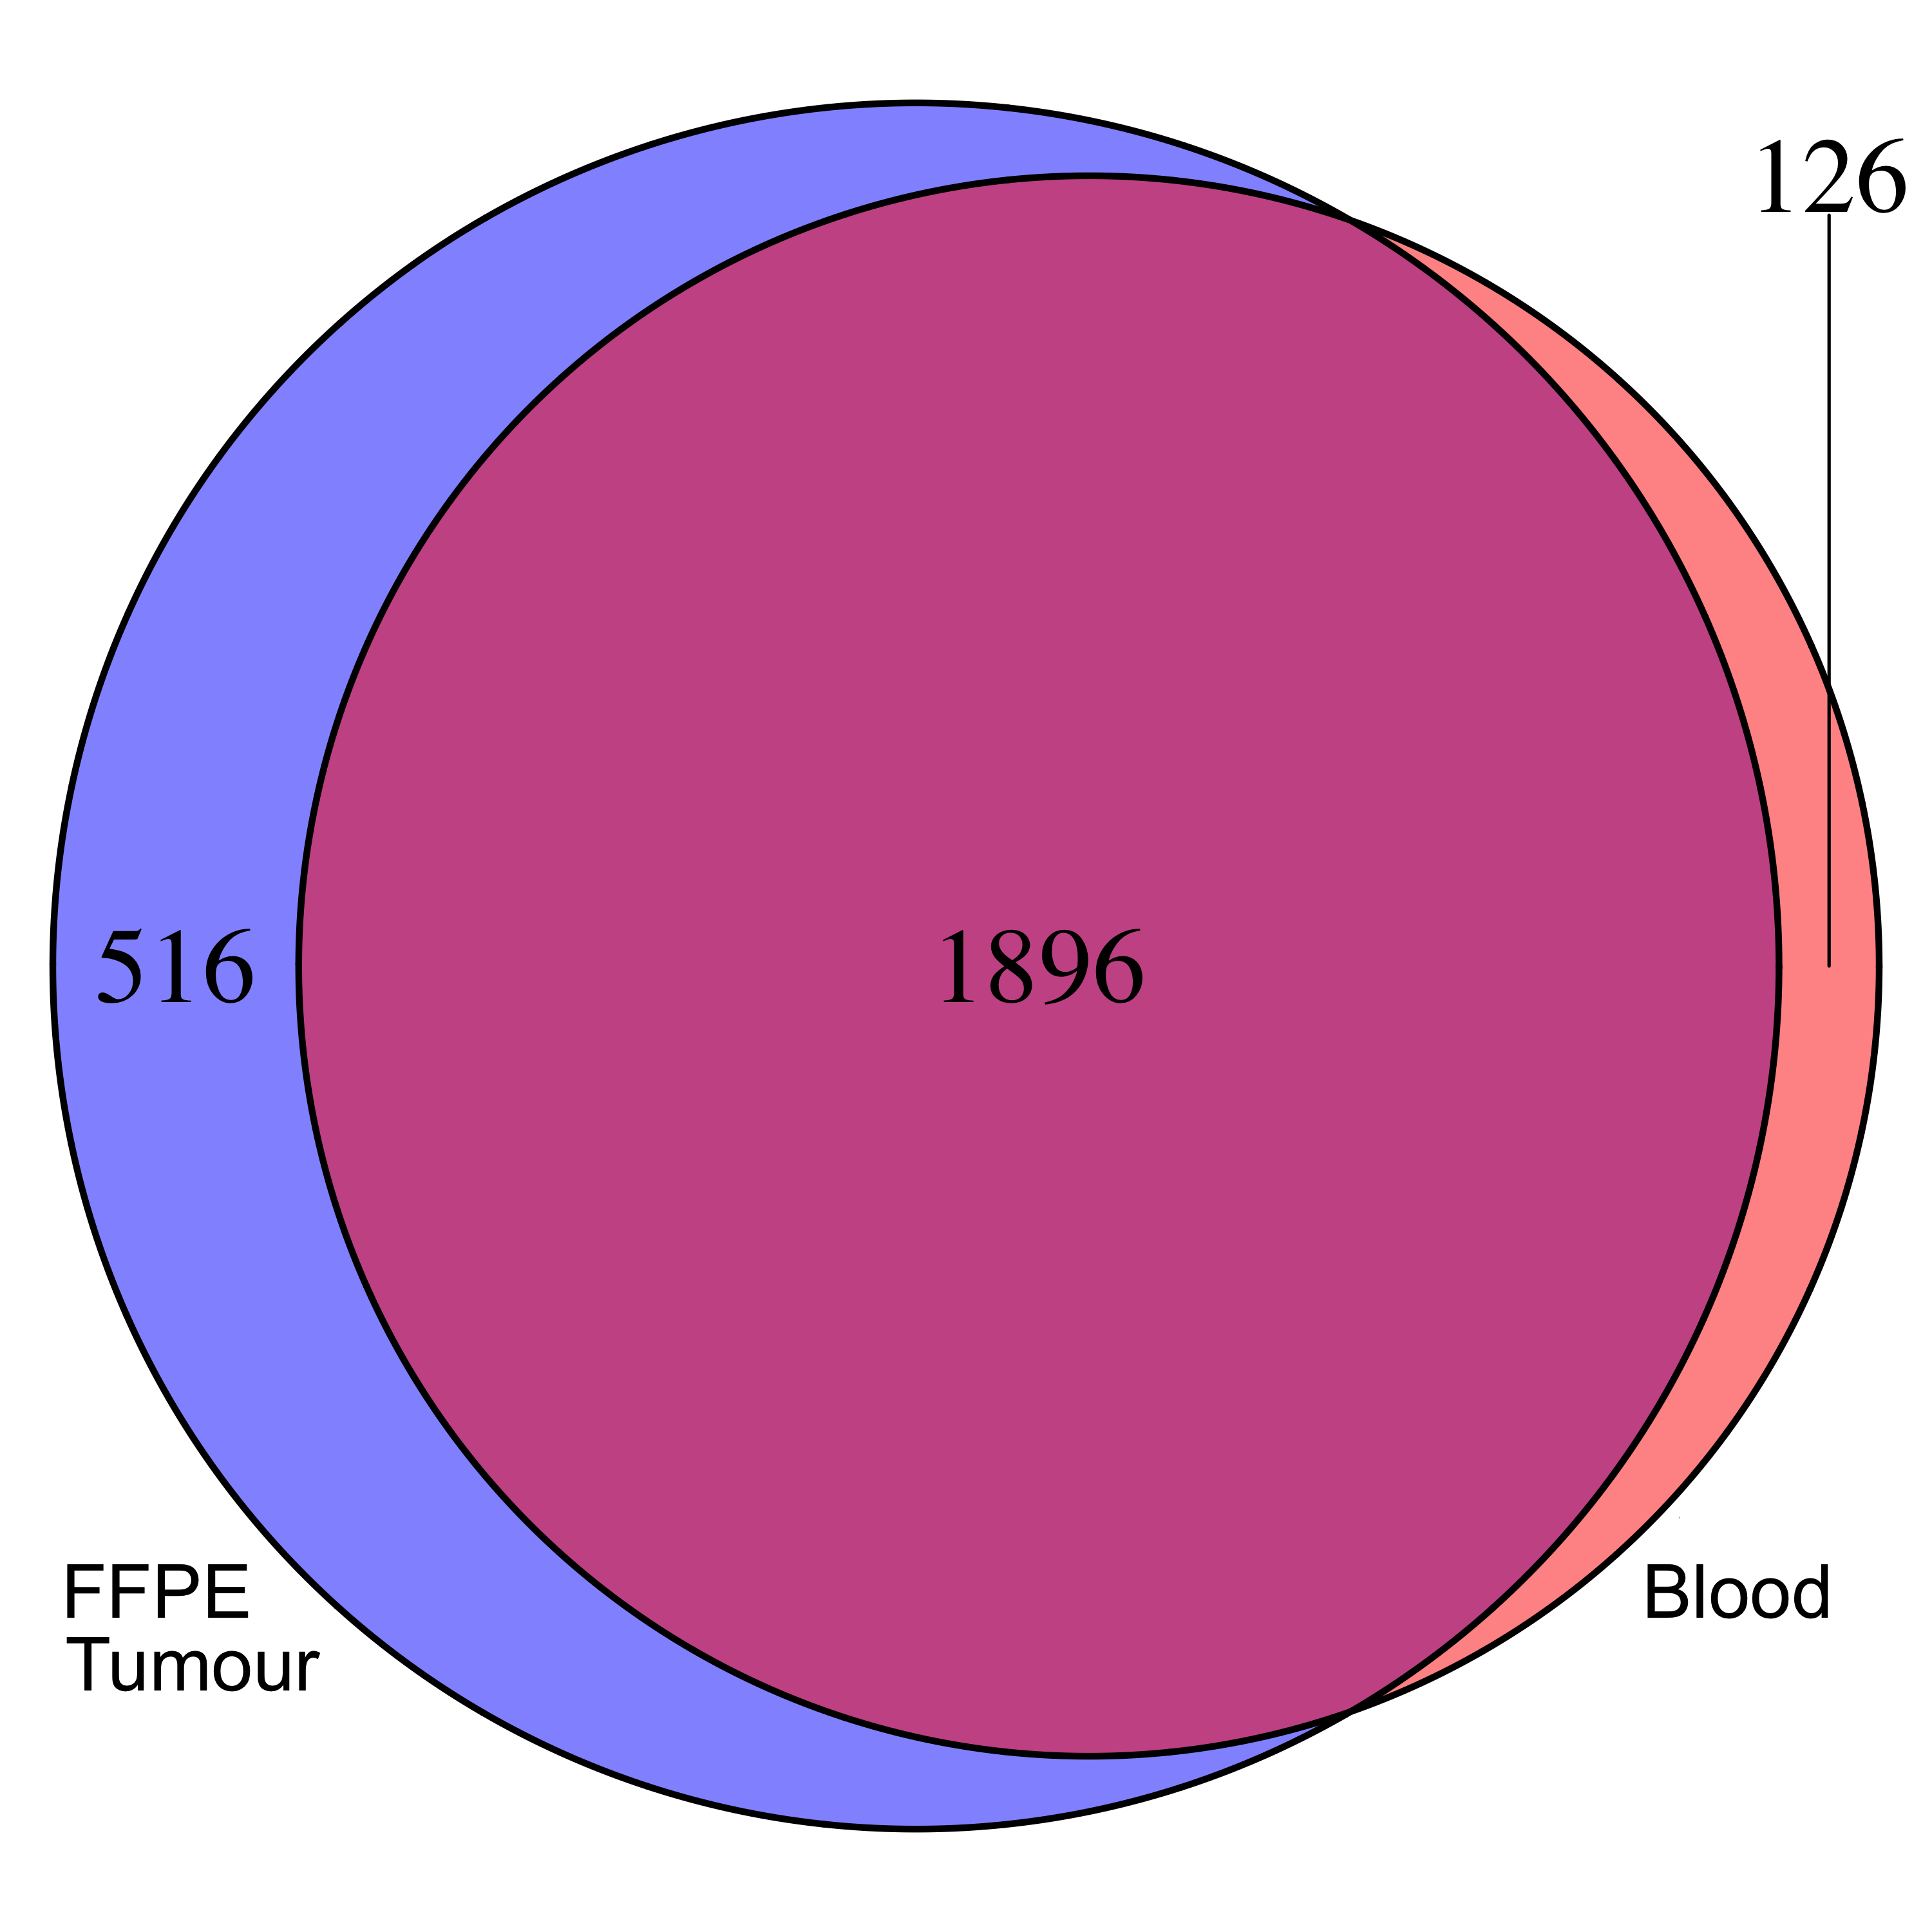
\includegraphics[scale=0.1]{ffpe_blood_conc_venn_gt.png}
	\caption{Venn diagram demonstrating concordance of variants identified in 217 tumour-blood paired samples.}
	\label{fig:ffpe_blood_conc_venn}
\end{figure}

%%%%%%%%%%%%%%%%%%%%%%%%%%%%%%%%%%%%%%%%%%%%%%%%%%%%%%%%%%%%%%%%%%%%%%
%%%%%%%%%%%%%%%%%%%%%%%%%%%%%%%%%%%%%%%%%%%%%%%%%%%%%%%%%%%%%%%%%%%%%%

\newpage
\begin{landscape}

\begin{longtable}{p{0.09\linewidth}|p{0.1\linewidth}p{0.12\linewidth}p{0.14\linewidth}p{0.17\linewidth}p{0.2\linewidth}p{0.06\linewidth}}
\caption{Distribution of discordant germline alterations identified in patients from TOP cohort.}
\label{tbl:freq_discordant_germline}
		\\
		\hline
		Gene & Chr:Pos & ID\textsuperscript{$\star$} & HGVS\textsuperscript{*} & Clinical Significance\textsuperscript{$\dagger$} & Reason for discordance & Count
		\\
		\hline
		DPYD & 1:97547947 & rs67376798 & p.Asp949Val c.2846A$>$T & Drug response & Het$/$WT & 1
		\\
		& 1:97770920 & rs1801160 & p.Val732Ile c.2194G$>$A & Benign$/$Likely benign, Not provided & Het$/$Hom & 2
		\\
		& 1:98165091 & rs2297595 & p.Met166Val c.496A$>$G & Drug response &  Het$/$Hom & 2
		\\
		& 1:98348885 & rs1801265 & p.Cys29Arg c.85T$>$C & Not provided & Low coverage in tumour & 2
		\\
		& 1:98348885 & rs1801265 & p.Cys29Arg c.85T$>$C & Not provided & Het$/$WT & 2
		\\
		& 1:98348885 & rs1801265 & p.Cys29Arg c.85T$>$C & Not provided & Het$/$Hom & 6
		\\
		\hline
		EGFR & 7:55249063 & rs1050171; COSM1451600 & p.Gln787Gln c.2361G$>$A & Benign$/$Likely benign & Het$/$Hom & 2
		\\
		\hline
		GSTP1 & 11:67352689 & rs1695 & p.Ile105Val c.313A$>$G & Drug response & Het$/$WT & 3
		\\
		& 11:67352689 & rs1695 & p.Ile105Val c.313A$>$G & Drug response & Het$/$Hom & 14
		\\
		\hline
		KIT & 4:55602765 & rs3733542; COSM1325 & p.Leu862Leu c.2586G$>$C & Benign$/$Likely benign & Het$/$Hom & 8
		\\
		\hline
		MTHFR & 1:11854476 & rs1801131 & p.Glu429Ala c.1286A$>$C & Drug response & Het$/$Hom & 12
		\\
		& 1:11856378 & rs1801133 & p.Ala222Val c.665C$>$T & Drug response & Het$/$Hom & 12
		\\
		& 1:11856378 & rs1801133 & p.Ala222Val c.665C$>$T & Drug response & Het$/$WT & 3
		\\
		\hline
		MTOR & 1:11169420 & rs41274506 & p.Asp2485Asp c.7455C$>$T & NA & Het$/$WT & 1
		\\
		& 1:11181327 & rs11121691 & p.Leu2303Leu c.6909G$>$A & NA & Het$/$Hom & 2
		\\
		& 1:11181327 & rs11121691 & p.Leu2303Leu c.6909G$>$A & NA & Low coverage in tumour & 1
		\\
		& 1:11181327 & rs11121691 & p.Leu2303Leu c.6909G$>$A & NA & Het$/$WT & 2
		\\
		& 1:11190646 & rs2275527 & p.Ser1851Ser c.5553C$>$T & Benign & Het$/$WT & 1
		\\
		& 1:11190730 & rs17848553 & p.Ala1823Ala c.5469C$>$T & Benign & Het$/$Hom & 4
		\\
		& 1:11205058 & rs1057079; rs386514433 & p.Ala1577Ala c.4731A$>$G & NA & Het$/$Hom & 8
		\\
		& 1:11205058 & rs1057079; rs386514433 & p.Ala1577Ala c.4731A$>$G & NA & Het$/$WT & 4
		\\
		& 1:1272468 & rs17036536 & p.Arg1154Arg c.3462G$>$C & Benign & Het$/$Hom & 4
		\\
		& 1:11288758 & rs1064261 & p.Asn999Asn c.2997T$>$C & NA & Het$/$Hom & 4
		\\
		& 1:11288758 & rs1064261 & p.Asn999Asn c.2997T$>$C & NA & Het$/$WT & 3
		\\
		& 1:11301714 & rs1135172 & p.Asp479Asp c.1437T$>$C & NA & Low coverage in tumour & 1
		\\
		& 1:11301714 & rs1135172 & p.Asp479Asp c.1437T$>$C & NA & Het$/$Hom & 8
		\\
		\hline
		PDGFRA & 4:55141055 & rs1873778; COSM1430082 & p.Pro567Pro c.1701A$>$G & Benign & Low coverage in tumour & 3
		\\
		& 4:55152040 & rs2228230; COSM22413 & p.Val824Val c.2472C$>$T & Benign & Het$/$WT & 2
		\\
		& 4:55152040 & rs2228230; COSM22413 & p.Val824Val c.2472C$>$T & Benign & Het$/$Hom & 4
		\\
		\hline
		STAT1 & 2:191872307 & rs45463799 & p.Asn118Asn c.354C$>$T & Likely benign & Het$/$WT & 1
		\\
		& 2:191874667 & rs386556119; rs2066802 & p.Leu21Leu c.63T$>$C & Benign & Het$/$WT & 1
		\\
		\hline
		STAT3 & 17:40498713 & NA & p.Lys49Lys c.147A$>$G & NA & Het$/$WT & 1
		\\
		\hline
		TP53 & 17:7577553 & COSM44368 & p.Met243fs c.727delA & NA & Het$/$WT & 1
		\\
		& 17:7579472 & COSM250061; rs1042522 & p.Arg72Pro c.215G$>$C & Drug response & Het$/$Hom & 26
		\\
		& 17:7579472 & COSM250061; rs1042522 & p.Arg72Pro c.215G$>$C & Drug response & Het$/$WT & 4
		\\
		& 17:7579579 & rs1800370 & p.Pro36Pro c.108G$>$A & Benign$/$Likely benign & Het$/$Hom & 2
		\\
		\hline
		TYMP & 22:50964236 & rs11479 & p.Ser471Leu c.1412C$>$T & Benign$/$Likely benign & Het$/$Hom & 14
		\\
		\hline
		TYMS & 18:673443 & rs151264360 & \footnotesize{c.*447\_*452delTTAAAG} & Drug response & Het$/$Hom & 32
		\\
		& 18:673443 & rs151264360 & \footnotesize{c.*447\_*452delTTAAAG} & Drug response & Het$/$WT & 1
		\\
		\hline
		UGT1A1 & 2:234668870 & rs873478 & c.-64G$>$C & NA & Het$/$WT & 1
		\\
		& 2:234668879 & rs34983651 & c.-55\_-54insAT & Conflicting interpretations of pathogenicity, Association & Hom$/$Het & 4
		\\
		& 2:234668879 & rs34983651 & c.-55\_-54insAT & Conflicting interpretations of pathogenicity, Association & Hom$/$WT & 2
		\\
		\hline
		\\
		&
		\multicolumn{5}{r}{Total discordant variants = 211}
		&
		\\
		\hline
\end{longtable}

%%%%%%%%%%%%%%%%%%%%%%%%%%%%%%%%%%%%%%%%%%%%%%%%%%%%%%%%%%%%%%%%%%%%%%
\noindent\textsuperscript{$\star$}dbSNP and/or COSMIC IDs.
\\
\textsuperscript{*}Description of sequence variants according to the HGVS recommendations.
\\
\textsuperscript{$\dagger$}Clinical significance on ClinVar database.
\\
Het$/$Hom = Loss of heterozygosity in the tumour
\\
Het$/$WT = Heterozygous in the blood, but wild type in the tumour
\\
Hom$/$Het = Homozygous in the blood, but heterozygous in the tumour

\end{landscape}

%%%%%%%%%%%%%%%%%%%%%%%%%%%%%%%%%%%%%%%%%%%%%%%%%%%%%%%%%%%%%%%%%%%%%%
\section{Application of VAF threshold to separate germline alterations from somatic mutations in tumour-only analyses}
\label{sec:ApplicationofVAFthresholdtoseparategermlinealterationsfromsomaticmutationsintumour-onlyanalyses}

Through variant analysis of DNA from blood specimens, we identified germline alterations that are associated with drug response, which could predict risk of developing chemotherapy-induced toxicity. Furthermore, we assessed the concordance of germline variants between blood and tumour samples, which demonstrated a high concordance rate of 93.8\%. Together, these analyses confirmed that germline alterations that are clinically relevant are present in our dataset and a large proportion of germline alterations can be identified in tumour DNA with the correct designation of allelic statuses. Next, we sought to evaluate the use of VAF thresholds to separate germline alterations from somatic mutations in tumour-only analyses. Because of the lack of availability of matched normal samples in clinical genomic sequencing, this assessment would determine whether application of VAF thresholds is an accurate method to identify potential germline alterations in clinical tumour sequencing for referral to follow-up testing. While our dataset does not contain pathogenic germline variants, we anticipate that this approach can be used to detect genetic events associated with cancer predisposition and drug response for future patients.

We compared the VAF distributions of germline variants detected in blood and tumour specimens, and we found a significant difference (Kolmogorov-Smirnov test, D = 0.17, \textit{p} = 0; \autoref{fig:germline_sens_minor}). As expected, we showed that heterozygous alterations in blood tend to have VAFs close to 50\%, whereas homozygous alterations in the blood tend to have VAFs close to 100\%. However, the VAF distribution of germline variants in the tumours tend to deviate from 50\% and 100\% for heterozygous and homozygous statuses, respectively. This variation in VAF distributions between blood and tumour samples, which could be caused by tumour content, tumour heterogeneity, or DNA damage as a result of formalin fixation, indicates that the sensitivity of using a VAF cut-off to distinguish between germline and somatic alterations in tumour-only analyses could be compromised. Thus, we explored the sensitivity of identifying germline alterations at various VAF thresholds to select a VAF cut-off that maximizes true positive rate. At each VAF cut-off, we determined the number of true positives by identifying variants in the tumours that overlap with germline variants in matched blood samples. True positive rate (sensitivity) is then calculated as the fraction of variants that are correctly identified as germline using the VAF threshold over the total number of germline variants in the tumours. At a VAF cut-off of 30\%, we achieved a sensitivity of 0.94 (95\% CI = 0.93--0.95; \autoref{fig:germline_sens_minor}; \autoref{tbl:sensitivity}), resulting in 1864 true positives and 117 false negatives out of a total of 1981 calls.

Because clinical genomics require accurate identification of genetic alterations that are clinically important, potential germline alterations identified through tumour-only analyses must be referred to follow-up testing \cite{Raymond2016, Bombard2014, Green2013}. Hence, not only must our approach for discriminating between germline and somatic alterations be highly sensitive, but also highly precise to minimize submission of somatic mutations (false positives) for downstream germline testing, which could incur additional cost and time. For similar reasons that cause VAFs of germline alterations in tumour samples to differ from germline alterations in the blood, we presumed VAFs of somatic mutations to be lower. We assessed this variation in VAF distributions between germline and somatic alterations in the tumours and found a significant difference (Kolmogorov-Smirnov test, D = 0.52, \textit{p} = 0; \autoref{fig:germline_ppv_minor}). Indeed, VAFs of somatic mutations tend to be concentrated at lower percentages compared to VAFs of germline variants. To select a VAF cut-off that would achieve high precision, we measured positive predictive values at various VAF thresholds. At each VAF cut-off, we identified true germline alterations by overlapping the variants in the tumours with germline variants called in matched blood samples. Positive predictive value is then calculated as the fraction of true positives over total number of variants identified in the tumours, including somatic mutations (false positives). At a VAF cut-off of 30\%, we achieved a positive predictive value of 0.90 (95\% CT = 0.89--0.91; \autoref{fig:germline_ppv_minor}; \autoref{tbl:ppv}), resulting in 1864 true positives and 203 false positives out of a total of 2067 calls.

Despite the difference in VAF distributions between germline alterations in blood and tumour samples, we managed to apply a VAF cut-off of 30\% to obtain a sensitivity of 0.94. This also means that this cut-off would result in a miss rate of 0.059 (95\% CI = 0.049--0.07), in which approximately 6\% of true germline variants will be missed. Moreover, we were also able to leverage the difference in VAFs of germline and somatic variants to distinguish germline variants from somatic mutations in tumour-only analyses. At the 30\% VAF cut-off, we were not only able to achieve sensitivity of 0.94, but also a positive predictive value of 0.90, meaning that close to 10\% of calls identified using this approach are somatic mutations. Overall, we demonstrated that the use of VAF threshold to identify potential germline alterations in clinical tumour sequencing is a promising approach towards mitigating challenges caused by the lack of matched normal samples and funding in the clinical setting.

%%%%%%%%%%%%%%%%%%%%%%%%%%%%%%%%%%%%%%%%%%%%%%%%%%%%%%%%%%%%%%%%%%%%%%
%%%%%%%%%%%%%%%%%%%%%%%%%%%%%%%%%%%%%%%%%%%%%%%%%%%%%%%%%%%%%%%%%%%%%%

\begin{figure}[H]
	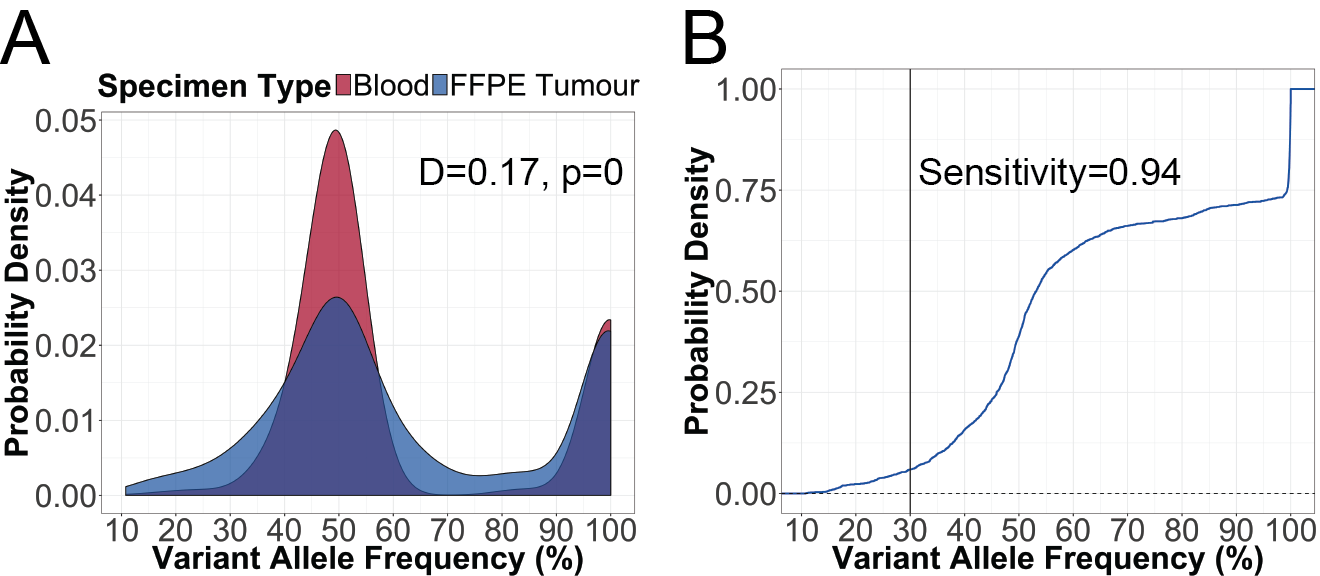
\includegraphics[scale=0.7]{germline_sens_minor.png}
	\caption[Assessment of using a VAF cut-off approach to identify germline alterations in tumour-only analyses.]{Assessment of using a VAF cut-off approach to identify germline alterations in tumour-only analyses. (A) Comparison of VAF distributions of germline alterations between blood and tumour (Kolmogorov-Smirnov test). (B) Empirical cumulative distribution of VAFs of germline alterations in tumour samples. Black line indicates VAF cut-off at 30\%, in which sensitivity of identifying germline variants is 0.94.}
	\label{fig:germline_sens_minor}
\end{figure}

%%%%%%%%%%%%%%%%%%%%%%%%%%%%%%%%%%%%%%%%%%%%%%%%%%%%%%%%%%%%%%%%%%%%%%
%%%%%%%%%%%%%%%%%%%%%%%%%%%%%%%%%%%%%%%%%%%%%%%%%%%%%%%%%%%%%%%%%%%%%%

\begin{table}[H]
\caption[Sensitivity of identifying germline variants in tumour-only analyses at various variant allele frequency thresholds.]{Sensitivity of identifying germline variants in tumour-only analyses at various variant allele frequency thresholds. 95\% confidence interval is the binomial confidence interval calculated using the Clopper-Pearson method.}
\label{tbl:sensitivity}
\centering
      \begin{tabular}{ccccl}
        \hline
        VAF (\%) & False Negative & True Positive & Sensitivity & 95\% CI
        \\
        \hline
        10 & 0 & 1981 & 1.0 & 1.0--1.0
        \\
        15 & 13 & 1968 & 0.99 & 0.99-1.0
        \\
        20 & 46 & 1935 & 0.98 & 0.97--0.98
        \\
        25 & 77 & 1904 & 0.96 & 0.95--0.97
        \\
        30 & 117 & 1864 & 0.94 & 0.93--0.95
        \\
        35 & 192 & 1789 & 0.90 & 0.89--0.92
        \\
        40 & 313 & 1668 & 0.84 & 0.83--0.86
        \\
        45 & 458 & 1523 & 0.77 & 0.75--0.79
        \\
				\hline
      \end{tabular} \\
\end{table}

%%%%%%%%%%%%%%%%%%%%%%%%%%%%%%%%%%%%%%%%%%%%%%%%%%%%%%%%%%%%%%%%%%%%%%
%%%%%%%%%%%%%%%%%%%%%%%%%%%%%%%%%%%%%%%%%%%%%%%%%%%%%%%%%%%%%%%%%%%%%%

\begin{figure}[H]
	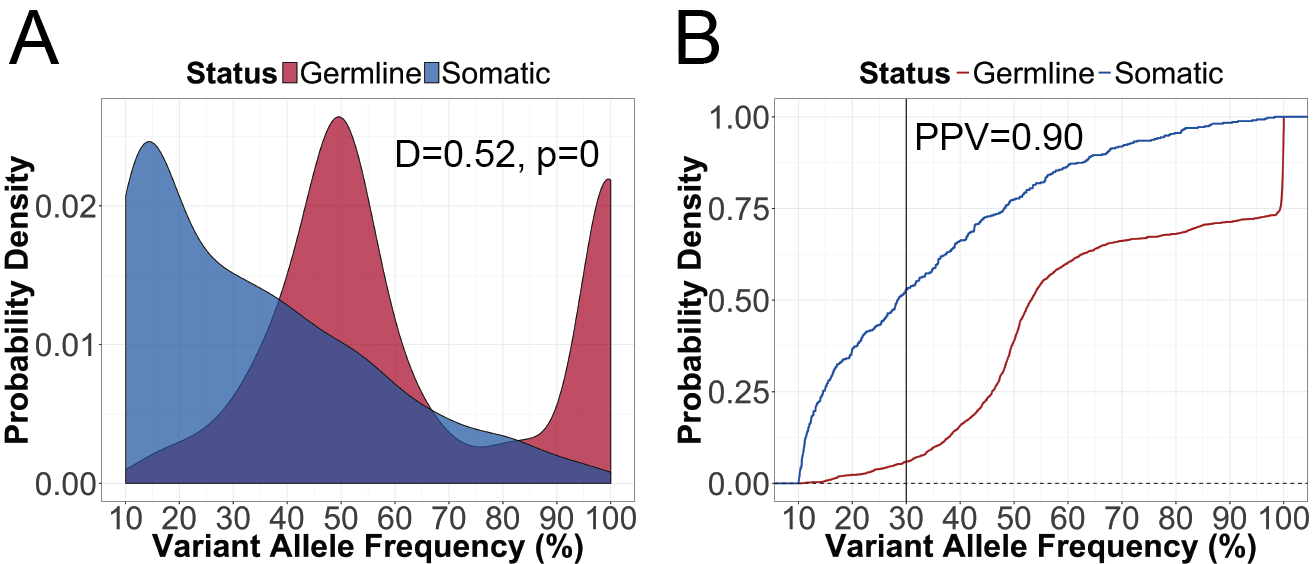
\includegraphics[scale=0.7]{germline_ppv_minor.png}
	\caption[Assessment of using a VAF cut-off approach to refer potential germline alterations in tumour-only analyses to follow-up testing.]{Assessment of using a VAF cut-off approach to refer potential germline alterations in tumour-only analyses to follow-up testing. (A) Comparison of VAF distributions between germline and somatic alterations in tumour specimens (Kolmogorov-Smirnov test). (B) Empirical cumulative distribution of VAFs of germline and somatic alterations in tumour samples. Black line indicates VAF cut-off at 30\%, in which positive predictive value of referring potential germline variants to follow-up testing is 0.90.}
	\label{fig:germline_ppv_minor}
\end{figure}

%%%%%%%%%%%%%%%%%%%%%%%%%%%%%%%%%%%%%%%%%%%%%%%%%%%%%%%%%%%%%%%%%%%%%%
%%%%%%%%%%%%%%%%%%%%%%%%%%%%%%%%%%%%%%%%%%%%%%%%%%%%%%%%%%%%%%%%%%%%%%

\begin{table}[H]
\caption[Positive predictive values for referral of potential germline variants to downstream confirmatory testing at various variant allele frequency thresholds.]{Positive predictive values for referral of potential germline variants to downstream confirmatory testing at various variant allele frequency thresholds. 95\% confidence interval is the binomial confidence interval calculated using the Clopper-Pearson method.}
\label{tbl:ppv}
\centering
      \begin{tabular}{cccccll}
        \hline
        VAF (\%) & False Positive & True Positive & Total Calls & Positive Predictive Value & 95\% CI
        \\
        \hline
        10 & 431 & 1981 & 2412 & 0.82 & 0.81--0.84
        \\
        15 & 319 & 1968 & 2287 & 0.86 & 0.85--0.87
        \\
        20 & 273 & 1935 & 2208 & 0.88 & 0.86--0.89
        \\
        25 & 245 & 1904 & 2149 & 0.89 & 0.87--0.90
        \\
        30 & 203 & 1864 & 2067 & 0.90 & 0.89--0.91
        \\
        35 & 178 & 1789 & 1967 & 0.91 & 0.90--0.92
        \\
        40 & 146 & 1668 & 1814 & 0.92 & 0.91--0.93
        \\
        45 & 118 & 1523 & 1641 & 0.93 & 0.91--0.94
        \\
				\hline
      \end{tabular} \\
\end{table}

%%%%%%%%%%%%%%%%%%%%%%%%%%%%%%%%%%%%%%%%%%%%%%%%%%%%%%%%%%%%%%%%%%%%%%
%%%%%%%%%%%%%%%%%%%%%%%%%%%%%%%%%%%%%%%%%%%%%%%%%%%%%%%%%%%%%%%%%%%%%%


%%%%%%%%%%%%%%%%%%%%%%%%%%%%%%%%%%%%%%%%%%%%%%%%%%%%%%%%%%%%%%%%%%%%%%
\endinput


Tumour-only sequencing is commonly performed by clinical laboratories to detect targetable somatic mutations, which can inform clinical decision making. Unlike the research setting, matched normal samples such as blood, saliva, or adjacent normal tissues are not routinely processed in the clinical setting due to limited sample availability, funding, and time \cite{Frampton2013, Fumagalli2010, Lin2014, Wong2014a}. The tumour genome also contains germline information that may have clinical implications for patients and their families. For instance, germline alterations in cancer-predisposing genes could facilitate implementation of cancer preventative measures such as early screening and sibling testing \cite{Schrader2015, Meric-Bernstam2016}. Moreover, germline PGx variants could predict response to drugs like chemotherapeutic agents, thereby preventing adverse drug reactions \cite{McLeod2013, Dai2008, Lee2014, Morel2006, VanKuilenburg2016, Etienne-Grimaldi2010, Mohelnikova-Duchonova2014, Jennings2013}.

Because the tumour genome consists of both germline and somatic alterations, it is important to establish approaches to distinguish between germline and somatic alterations in cancer diagnostic assays that only sequence tumour DNA. In the absence of matched normal samples, approaches such as constructing a virtual normal by combining variants identified in multiple normal samples from healthy individuals and filtering variants using public databases such as such as dbSNP, 1000 Genomes Project, and COSMIC could enable the differentiation of germline variations from somatic mutations \cite{Hiltemann2015, Jones2015a}. Subsequently, potential germline alterations can be referred to follow-up testing, which involves genetic counseling and collection of germline samples for further sequencing and analysis \cite{Raymond2016, Bombard2014, Green2013}.

The TOP study is comprised of 213 patients with tumour and matched blood specimens. We annotated the germline variants identified in blood specimens from TOP patients using the effect prediction software, SnpEff (version 4.2), and ExAC and 1000 Genomes databases, which provide information on population frequency. We also interpreted the variant calls with the ClinVar database, which enable assessment of clinical significance. Furthermore, we performed manual literature review to determine the functional and clinical impacts of all germline alterations detected in the blood samples. Because several studies demonstrated that a germline cancer-predisposing variant is present in 3-10\% of patients undergoing tumour-normal sequencing \cite{Raymond2016,Meric-Bernstam2016,Schrader2015,Jones2015a}, we sought to confirm the presence of germline alterations in the tumour genome by measuring variant concordance between blood and tumour DNA. This enables us to determine whether tumour DNA is a reliable substrate for identification of germline alterations.

Lastly, we differentiated between germline and somatic statuses of variants identified in tumour DNA through applying VAF thresholds. While heterozygous germline variants are expected to have VAF of close to 50\%, homozygous germline variants are expected to have VAF of close to 100\%. In contrast, the VAF of somatic mutations relies on tumour purity. Due to contamination of normal tissues in tumour specimens, it is highly likely that the VAFs of somatic mutations are substantially lower than the expected VAFs for germline alterations \cite{}. Furthermore, other factors such as tumour heterogeneity and formlin-induced DNA damage could cause deviation of somatic VAFs from the expected 50\% and 100\% for heterozygous and homozygous variants, respectively \cite{}. As we have matched blood samples for all tumour samples, we were able to evaluate the sensitivity of using VAF thresholds to discriminate between germline and somatic alterations in tumour DNA. Furthermore, we also assessed the positive predictive value of referring potential germline alterations for follow-up testing. Through these analyses, we hope to establish a VAF cut-off that could maximize true positive rate for identification of potential germline alterations, as well as minimize false positive rate to reduce unnecessary follow-up testing, which could cause patients preventable psychological distress and hassles.

Together, our analyses would provide insights on whether application of VAF thresholds is a practical approach to distinguish between germline and somatic alterations in tumour-only sequencing assays. Hence, this will determine whether tumour-only sequencing assays can be leveraged by clinical laboratories for initial screening of germline alterations that are clinically relevant.


Look at PGx variants with drug response and calculate the probability of not achieving 30\% VAF.

\pagebreak

\begin{table}[H]
\caption{Frequency of germline and somatic variants detected in the tumours of 213 patients in the TOP cohort.}\label{freqvariants}
\centering
\begin{tabular}{lcclcl}
        \hline
        Gene & Germline & Pathogenic Germline && Somatic \\
				 & (N Patients) & (N Patients) && (N Patients) \\
				\hline
				\\
				\multicolumn{1}{l}{\textit{Cancer predisposing}}
				&
				\multicolumn{2}{l}{ }
				&&
				\multicolumn{1}{l}{} \\
				\hline
				AKT1 & 0 & 0 && 2 (2) \\
				\arrayrulecolor{evagrey}\hline
				ALK & 1 (1) & 1 (1) && 2 (1) \\
				\hline
				BRAF & 0 & 0 && 18 (17) \\
				\hline
				EGFR & 170 (164) & 5 (5) && 31 (24) \\
				\hline
				HRAS & 0 & 0 && 1 (1) \\
				\hline
				MAP2K1 & 0 & 0 && 2 (2) \\
				\hline
				MAPK1 & 17 (17) & 3 (3) && 3 (2) \\
				\hline
				MTOR & 763 (213) & 6 (6) && 71 (30) \\
				\hline
				NRAS & 0 & 0 && 8 (8) \\
				\hline
				PDGFRA & 242 (185) & 0 && 8 (4) \\
				\hline
				PIK3CA & 0 & 0 && 15 (4) \\
				\hline
				PTEN & 0 & 0 && 1 (1) \\
				\hline
				STAT1 & 54 (51) & 1 (1) && 7 (6) \\
				\hline
				STAT3 & 10 (10) & 4 (4) && 16 (11) \\
				\hline
				TP53 & 189 (184) & 2 (2) && 131 (109) \\
				\arrayrulecolor{black}\hline
				\\
				\multicolumn{1}{l}{\textit{Pharmacogenomics}}
				&
				\multicolumn{2}{l}{ }
				&&
				\multicolumn{1}{l}{} \\
				\arrayrulecolor{black}\hline
				DPYD & 271 (212) & 1 (1) && 1 (1) \\
				\arrayrulecolor{evagrey}\hline
				GSTP1 & 106 (106) & 0 && 0 \\
				\hline
				MTHFR & 209 (177) & 0 && 0 \\
				\hline
				TYMP & 81 (76) & 2 (2) && 18 (13)\\
				\hline
				TYMS & 131 (131) & 0 && 0 \\
				\hline
				UGT1A1 & 96 (96) & 0 && 1 (1) \\
				\arrayrulecolor{black}\hline \\
				Total & 2396 (213*) & 25 (23*) && 431 (180*) \\
				\arrayrulecolor{black}\hline
      \end{tabular}
\end{table}


%    5. Discussion
%% The following is a directive for TeXShop to indicate the main file
%%!TEX root = diss.tex

%%%%%%%%%%%%%%%%%%%%%%%%%%%%%%%%%%%%%%%%%%%%%%%%%%%%%%%%%%%%%%%%%%%%%%
\chapter{Discussion}
\label{ch:Discussion}
%%%%%%%%%%%%%%%%%%%%%%%%%%%%%%%%%%%%%%%%%%%%%%%%%%%%%%%%%%%%%%%%%%%%%%

Genomic analyses of tumours can reveal druggable somatic mutations, as well as clinically relevant germline alterations that are beneficial to patients and their family members \cite{Meric-Bernstam2016, Schrader2015, Jones2015a}. While sequencing of tumour-normal pairs can enable differentiation between germline and somatic variants, matched normal samples are often not obtained in clinical practice. Moreover, FFPE tumour tissues represent another challenge in clinical genomics. Formalin fixation damages nucleic acid through fragmentation and cytosine deamination, which affect molecular testing with FFPE DNA \cite{Do2015a, Kim2017, Ofner2017, Oh2015, Wong2013, Wong2014, Sikorsky2007}. Hence, usability of FFPE DNA for germline testing and approaches to discriminate between germline and somatic variants in tumour-only analyses must be evaluated. These assessments would facilitate optimization of workflows to identify potential germline alterations using clinical tumour sequencing.

In this study, we retrospectively analyzed targeted sequencing data from tumour and matched blood specimens of 213 cancer patients. Our findings demonstrated that DNA fragmentation and cytosine deamination were common forms of DNA damage in FFPE specimens. While the impact of formalin fixation on amplicon enrichment and sequencing results was detectable, we determined that these discrepancies were either technically negligible or could be minimized using appropriate methods. We also found that the majority of germline alterations identified in blood using our panel test were present with the same allelic statuses in FFPE tumours. This implies that a high proportion of germline genetic changes are retained in the tumour genome, demonstrating the reliability of using tumour DNA for germline variant calling. Finally, we assessed the application of VAF threshold to delineate germline and somatic variants in tumour-only analyses. We reported that a VAF cut-off of 30\% would correctly identify 94\% of germline alterations, while erroneously submit 10\% of false positives, which are somatic mutations, for follow-up germline testing. Because our gene panel and patient cohort are relatively small, we were only able to identify germline variants that are predictive of drug response. However, we surmised that application of this VAF cut-off could be expanded to predict the statuses of pathogenic germline variants such as alterations in \textit{BRCA} genes.

\subsection{Effects of formalin-induced DNA damage on sequencing metrics are minor and technically insignificant}

Several studies have reported findings that are consistent with our assessment of formalin-induced DNA damage in FFPE specimens. To assess the usability of FFPE DNA for germline testing, we compared efficiency in amplicon enrichment and sequencing results of FFPE DNA to blood, which is a gold standard for germline testing. We noted lower efficiency in amplicon enrichment in FFPE DNA, with a more pronounced decrease in coverage depth for longer amplicons in the panel. Similarly, Shi et al. \cite{Shi2002}, Didelot et al. \cite{Didelot2013}, and Wong et al. \cite{Wong2013} demonstrated that shorter amplicons gave rise to better PCR amplification success in FFPE DNA, indicating the presence of fragmentation damage, which yields template DNA of shorter fragment lengths. While we observed comparable proportion of on-target aligned reads between FFPE and blood DNA, there were minor discrepancies in coverage depth and uniformity of target bases in FFPE DNA. Various groups have also reported disparities in coverage depth and uniformity in FFPE DNA when compared to DNA extracted from either fresh frozen or unfixed specimens \cite{Wong2013, Betge2015, Spencer2013}. Additionally, Wong et al. \cite{Wong2014} and Didelot et al \cite{Didelot2013} showed inverse correlations between coverage depth and the degree of DNA fragmentation in FFPE DNA, suggesting that formalin-induced fragmentation damage could be accountable for such discrepancies in sequencing results. Although we detected differences in sequencing results between FFPE and blood DNA, we concluded that these effects were minor and technically insignificant. As for the discrepancy in amplicon enrichment, shorter amplicons can be designed to circumvent the drawback of fragmentation damage in FFPE samples.

\subsection{Impact of artifactual base changes on germline variant calling can be mitigating by applying a VAF cut-off}

Cytosine deamination is a major cause of sequence artifacts in formalin-fixed specimens \cite{Wong2014, Do2012, Oh2015, Spencer2013, Do2013, Kim2017, Chen2014}. Herein, we observed increased C$>$T/G$>$A artifacts in FFPE DNA compared to blood. Artifactual C$>$T/G$>$A changes are formed by incorporation of adenines in the complementary DNA strand at uracil lesions generated by deamination of cytosines \cite{Do2015a}. When measuring frequency of sequence artifacts at different allele frequency ranges, Wong et al. \cite{Wong2014} reported higher C$>$T/G$>$A transitions at a lower allele frequency range (1--10\% \textit{vs.} 10--25\%). This finding led us to compare the fraction of base changes at different allele frequency ranges, including 1--10\%, 10--20\%, and 20--30\%. Indeed, we observed a substantial increase in C$>$T/G$>$A within the 1--10\% allele frequency range. Considering that our goal is to predict germline status, disproportionate base changes between FFPE and blood DNA within these allele frequency ranges suggest that germline calls should be made at $>$ 30\% VAF to avoid false positives that could either arise from true somatic mutations or FFPE artifacts. We were unable to separate FFPE artifacts from low-allelic-fraction somatic mutations within these allele frequency ranges due to the lack of matched fresh frozen or unfixed tumour tissues. Nevertheless, somatic mutations can occur at VAFs that deviate significantly from a diploid zygosity (i.e. heterozygous variant should have VAF close to 50\%, whereas homozygous variant should have VAF close to 100\%) because of low tumour content or tumour heterogeneity \cite{Kim2017a, Xu2017, Carrot-Zhang2016, Tian2015, Cai2016}. Therefore, further workflow optimization should be performed for the purpose of identifying clinically relevant somatic mutations in the tumour genome. A method to reduce sequence artifacts caused by cytosine deamination is through treatment with uracil-DNA glycosylase (UDG) before sequencing. UDG is an enzyme capable of depleting uracil lesions in DNA, giving rise to abasic sites. During PCR amplification, cytosine bases are restored at abasic sites by using the complementary DNA strand as template, which consists of guanine bases opposite of the uracil lesions \cite{Do2015a}. Several studies showed that pre-treatment of FFPE DNA with UDG can markedly reduce C$>$T/G$>$A sequence artifacts \cite{Do2013, Kim2017, Do2012}. However, this approach cannot correct sequence artifacts at CpG dinucleotides because these cytosines are typically methylated, and deamination of 5-methyl cytosines generates thymines instead uracil bases, which are resistant to UDG repair \cite{Do2013}.

\subsection{Sequence artifacts other than those caused by cytosine deamination are detected}

We also observed elevated levels of A$>$G/T$>$C artifacts in FFPE DNA, albeit to a lesser extent compared to C$>$T/G$>$A artifacts. Likewise, Wong et al. \cite{Wong1998} reported that 35\% of sequence artifacts in Sanger sequencing of the \textit{BRCA1} gene were A$>$G/T$>$C nucleotide changes. We speculate that increase in A$>$G/T$>$C artifacts is caused by deamination of adenine to generate hypoxanthine, which forms base pairs with cytosine instead of thymine. This results in transformation of A-T base pairs to G-C base pairs. Deamination of adenine to hypoxanthine can be catalyzed by an acidic environment \cite{Wang2010}, which can arise in FFPE specimens because formaldehyde can be oxidized to generate formic acid \cite{Do2015a}. Acidic conditions also promotes depurination, creating abasic sites. Many DNA polymerases selectively incorporate adenines across abasic sites, while guanines and small deletions are integrated in fewer cases \cite{Heyn2010}. Despite statistically insignificant, we observed a subset of FFPE specimens with higher fractions of C$>$A/G$>$T artifacts. These artifactual changes could have resulted from depurination of guanines, followed by incorporation of adenines by DNA polymerase in the complementary strand, which alters G-C base pairs to A-T base pairs. Heyn et al. \cite{Heyn2010} reported that DNA polymerases demonstrated varying bypass rates at abasic sites. For instance, AmpliTaq Gold, \textit{Pfu}, and Platinum Taq HiFi extended across lower frequency of abasic sites compared to Platinum Taq, \textit{Bst} and \textit{Sso}-Dpo4 ($<$34\% \textit{vs.} $>$77\%) \cite{Heyn2010}. Thus, selection of a high fidelity DNA polymerase could lessen these forms of sequence artifacts. Costello et al. \cite{Costello2013} discovered that C$>$A/G$>$T artifacts can also occur due to oxidation of DNA during the shearing process, converting guanines to 8-oxoguanine lesions. This conversion is highly dependent on the surrounding 5' and 3' bases of the guanine, in which guanines within GGC are the most susceptible to oxidation. 8-oxoguanine can form base pairs with cytosine and adenine, and mispairing with adenine would give rise to artifactual C$>$A/G$>$T transversions. However, this was not the cause of C$>$A/G$>$T artifacts in our data because both blood and FFPE DNA were sheared, and we did not observe simultaneous C$>$A/G$>$T increments in both specimen types compared to other types of base changes.

\subsection{Storage time of FFPE blocks correlates with the extent of formalin-induced DNA damage}

Ludyga et al. \cite{Ludyga2012} demonstrated that long-term storage of FFPE blocks led to increased DNA fragmentation, producing shorter template DNA for PCR amplification. Furthermore, Carrick et al. \cite{Carrick2015} showed that increased storage time of FFPE blocks affects sequencing coverage and depth in NGS data. These findings are in agreement with our results, in which we found negative associations between age of paraffin blocks and efficiency in amplicon enrichment, coverage depth of target bases, and percentage of on-target aligned reads. As well, we observed a positive correlation between age of paraffin blocks and fraction of C$>$T/G$>$A artifacts, an outcome of stochastic enrichment. Due to exposure to environmental conditions, older FFPE blocks tend to produce increasingly fragmented DNA, which results in lower amounts of amplifiable DNA. Consequently, there is a higher chance of amplifying template DNA with sequence artifacts caused by formalin, yielding increased frequency of artifactual nucleotide changes in older FFPE specimens \cite{Wong2014}. These results demonstrating the correlations between storage time of paraffin blocks and sequencing variables suggest that if multiple FFPE blocks are available, the specimen with the shorter storage time should be selected for molecular testing. However, clinical specimens are often limited, making sample selection a rare option in the diagnostic setting. As such, other approaches to eliminate sequence artifacts should be considered such as application of molecular barcodes and hybridization-capture enrichment, which allow tracking of DNA templates \cite{Eijkelenboom2016, Samorodnitsky2015, Peng2015, Wong2013}. This would enable detection of variants that are only supported by the same template DNA, indicating a higher chance that these variants are sequence artifacts and should be interpreted with caution.

\subsection{Germline variants are highly retained in the tumour genome}

Various groups have identified clinically significant germline alterations through analyzing tumour genomes \cite{Schrader2015, Meric-Bernstam2016, Jones2015a, WcWhinney2009}. Schrader et al. \cite{Schrader2015} reported that potential pathogenic germline variants in cancer-predisposing genes were conserved in the tumours of 91.9\% of patients in their study cohort (182 of 198 patients), whereas 21.4\% of these patients (39 of 182 patients) demonstrated LOH or other forms of mutations in the remaining wild type allele. We found that 93.8\% of germline alterations identified in the blood were retained in the tumour with the same allelic statuses, a finding that is in line with previous work. This suggests that tumour DNA could be a reliable substrate for detecting germline alterations, implying that a tumour-only sequencing protocol could be leveraged for pre-screening of germline variants before submission to downstream confirmatory testing. A framework as such could provide germline testing in a cost-effective manner because only selective patients (i.e. those with potential germline alterations that are clinically important) would require follow-up. We also identified discordant germline variants between blood and tumour DNA, which were caused by various reasons like LOH, low sequencing coverage ($<$ 100x), and loss of variant allele in the tumours. All tumour specimens in our study were formalin-fixed, therefore it is possible that DNA damage induced by formaldehyde exposure played a role in creating discordant germline variants. Variant discordance can also be caused by mutagenesis in the tumour, such as somatic CNVs in the region of the germline variant. For instance, Gross et al. \cite{Gross2013} showed a high prevalence of \textit{DPYD} CNVs in high-grade triple negative breast cancer, particularly in cases with copy number loss of the \textit{BRCA1} DNA-repair gene. The common fragile site FRA1E is located within the \textit{DPYD} gene and its stability is highly dependent on intact \textit{BRCA1} \cite{Arlt2004}. Hence, deficiency in \textit{BRCA1} protein would result in increased fragility of FRA1E, leading to genomic rearrangements in \textit{DPYD}. As germline variants in the \textit{DPYD} gene can predict susceptibility to 5-FU-related toxicity, somatic CNVs in \textit{DPYD} could affect the detection of these germline variants in tumour genomic sequencing.

\subsection{The use of VAF threshold is feasible for distinguishing between germline and somatic alterations in tumour-only analyses}

Although sequencing of tumour-normal pairs would enable accurate identification of germline and somatic variants, this approach is not routinely practice in clinical genomics due to inadequate funding and facilities to store additional specimens. Methods to distinguish between germline and somatic alterations in tumour-only analyses have been described by different groups \cite{Hiltemann2015, Jones2015a, Garofalo2016}. Hiltemann et al. \cite{Hiltemann2015} used a virtual normal that was assembled by aggregating whole-genome-sequenced normal samples from 931 healthy and unrelated individuals, whereas Jones et al. \cite{Jones2015a} resorted to using an unmatched normal sample and public databases such as dbSNP, 1000 Genomes Project, and COSMIC, as well as effect prediction tools. We leveraged the fact that the VAFs of somatic mutations typically deviate from 50\% and 100\% for heterozygous and homozygous variants, respectively, and employed VAF threshold to differentiate between variant statuses. Our approach managed to achieve high sensitivity and precision, therefore verifying the feasibility of using VAF threshold to differentiate between germline and somatic alterations in the absence of matched normal samples. The VAF threshold method takes advantage of genetic impurity and heterogeneity of tumours, which render the deviation of somatic VAFs from diploid zygosity. Jones et al. \cite{Jones2015a} discovered that performance of the VAF threshold approach was highly dependent on tumour purity. While the use of VAF threshold can correctly identify germline and somatic alterations in tumours with $<$ 50\% purity, this accuracy was not observed for specimens with higher tumour content. In fact, only 12.5\% of cancer-predisposing germline variants and an average of 48\% of somatic mutations were accurately predicted \cite{Jones2015a}. Unfortunately, pathologic estimation of tumour content was not available for our analyses. However, we speculate that the tumour specimens in our dataset are highly impure or heterogeneous, thereby contributing to the high sensitivity and precision attained by the VAF threshold approach. While there are bioinformatic algorithms available to infer clonality and impurity estimates of tumours, many of these methods require matched normal controls or are not compatible with targeted sequencing data \cite{Yadav2015}. Nevertheless, this information should be integrated into clinical pipelines to enhance the performance of using a VAF threshold approach to distinguish between germline and somatic alterations in the course of analyzing tumour genomes without matched normal samples.

\subsection{Limitations and future directions}

There are several limitations in our study. First, we did not manually review every single variant called by our pipeline. Only variants located within primer regions were manually inspected, while our variant filter also included common artifacts that were curated during clinical assessment. Hence, it is highly possible that sequence artifacts are present in our dataset, particularly low-allelic-fraction variants (i.e. $<$ 30\%) detected in the blood. These potentially artifactual variants account for 6\% of all germline variants identified in blood DNA, thereby compromising sensitivity of the VAF threshold method. Variant inspection using a genome browser is routinely conducted by genomic analysts in clinical practice to decrease the risk of reporting false positive results \cite{Strom2016, Garofalo2016}. However, manual review of variants was not implemented in our study because our analyses were focused on evaluating analytical validity instead of inferring clinical implications of the variants called. Moreover, the large number of variants in our study would be time-consuming and unfeasible for manual inspection. Our evaluation of the VAF threshold approach in differentiating between germline and somatic variants is favourable of the framework to implement initial screening for germline variants in clinical tumour sequencing before follow-up germline testing. The relatively small gene panel and cohort size of our study are caveats in drawing this conclusion. Although we were able to identify germline variants that can influence drug response, we did not report any pathogenic germline variants that are associated with cancer predisposition in our dataset. Hence, we can only speculate that our approach could be applicable to variants in cancer-predisposing genes. Studies that were able to identify pathogenic germline variants were performed with cohort sizes and gene panels that are substantially larger than ours. For instance, the study by Schrader et al. \cite{Schrader2015}, which revealed pathogenic germline variants in 16\% of patients, was performed in a cohort of 1566 patients and screened for 341 genes. To determine whether the VAF threshold method can be applied to detect genetic alterations linked to cancer susceptibility, further assessment which involves a larger patient cohort and surveying known cancer-predisposing genes must be carried out.

The present study addresses two problems faced by using tumour genomic sequencing to identify germline alterations: the widespread use of FFPE tumours and the lack of matched normal samples. Archival FFPE tissues remain a sizable resource for cancer genomic studies and clinical genomic sequencing. Thus, there is a need to understand the extent of the different forms of DNA damage induced by formalin. Our analyses not only provide insights on the impact of formalin-induced DNA damage on amplicon-based NGS data, but also help us devise guidelines to minimize these effects. Formalin fixation followed by paraffin embedding is an attractive method to preserve tissues for histologic assessment because it allows storage at ambient temperature, which reduces cost that could be incurred by maintaining freezers required for fresh-frozen samples. Yet, many studies, including ours, have indicated the side effects of the formaldehyde exposure on nucleic acid \cite{Do2015a, Kim2017, Ofner2017, Oh2015, Wong2013, Wong2014, Sikorsky2007}. Instead of investing efforts into mitigating these side effects, a potential solution is to transition from the use of formalin to the UMFIX (Sakura Finetek USA, Inc.) fixative, which is capable of preserving both cellular morphology for pathologic review and macromolecules, including DNA \cite{Vincek2003}. Most clinical laboratories conduct tumour-only sequencing and apply approaches to distinguish between germline and somatic alterations. Without matched normal samples, interpretation of variants becomes complicated. Jones et al. \cite{Jones2015a} and Garofalo et al. \cite{Garofalo2016} concluded that sequencing of tumour-normal pairs is the best practice to accurately identify variant statuses. For a center to provide this service, it must be equipped to collect, analyze, and report germline findings. This includes establishing appropriate pre-test and post-test counseling, protocols to secure patient consent and manage variant of uncertain significance, and frameworks to communicate results that may implicate the patients' relatives. While various groups recommend the sequencing of tumour-normal pairs, some centers simply do not have the funding or infrastructure to implement this as a standard practice. Furthermore, the American College of Medical Genetics and Genomics (\acs{ACMG}) recommended that clinical laboratories report incidental variants in 56 genes that are associated with disease risk in DNA derived from germline samples, including matched normal samples that only serve the purpose of subtracting germline variants to identify somatic mutations in tumours \cite{Green2013}. Interrogation of these genes suggested by the ACMG guidelines could result in detection of more variants with uncertain significance, which might pose more harm than good to patients. Additionally, cases in which only FFPE tumour blocks exist for a deceased patient would greatly benefit from approaches in differentiating between germline and somatic variants. For example, if the deceased individual is suspected to be a carrier of an inheritable disease, the ability to accurately identify the germline risk allele could prompt germline testing for the individual's relatives and facilitate preventive care. Thus, establishing approaches to tell apart germline and somatic variants in tumour genomic analyses still has its advantages from clinical and financial perspectives.

To summarize, we confirmed that the common forms of formalin-induced DNA damage in our data were DNA fragmentation and cytosine deamination. Because these effects were either minor or technically insignificant, this justifies the use of FFPE DNA for germline testing. Characterization of formalin-induced DNA damage also assist in devising recommendations to enhance amplicon enrichment and sequencing results. We also reported a high retention rate of germline alterations in the tumour genome, suggesting the reliability of using tumour DNA for germline variant calling. Finally, we showed that application of VAF threshold can achieve high sensitivity and precision in distinguishing germline alterations from somatic mutations in tumour-only analyses. This supports the framework of leveraging clinical tumour sequencing for initial germline testing. Subsequently, only patients with potential germline variants will be referred to follow-up testing. A framework as such represents a cost-effective way to deliver germline testing because only selective patients will require downstream testing. Nevertheless, extrapolation of this approach for discriminating between germline and somatic variants in cancer-predisposing genes needs further evaluation.


%    6. Conclusion
% %% The following is a directive for TeXShop to indicate the main file
%%!TEX root = diss.tex

\chapter{Conclusion}
\label{ch:Conclusion}

What are my main findings?



%    2. Main body
% Generally recommended to put each chapter into a separate file
%\include{relatedwork}
%\include{model}
%\include{impl}
%%% The following is a directive for TeXShop to indicate the main file
%%!TEX root = diss.tex

%%%%%%%%%%%%%%%%%%%%%%%%%%%%%%%%%%%%%%%%%%%%%%%%%%%%%%%%%%%%%%%%%%%%%%
\chapter{Discussion}
\label{ch:Discussion}
%%%%%%%%%%%%%%%%%%%%%%%%%%%%%%%%%%%%%%%%%%%%%%%%%%%%%%%%%%%%%%%%%%%%%%

Genomic analyses of tumours can reveal druggable somatic mutations, as well as clinically relevant germline alterations that are beneficial to patients and their family members \cite{Meric-Bernstam2016, Schrader2015, Jones2015a}. While sequencing of tumour-normal pairs can enable differentiation between germline and somatic variants, matched normal samples are often not obtained in clinical practice. Moreover, FFPE tumour tissues represent another challenge in clinical genomics. Formalin fixation damages nucleic acid through fragmentation and cytosine deamination, which affect molecular testing with FFPE DNA \cite{Do2015a, Kim2017, Ofner2017, Oh2015, Wong2013, Wong2014, Sikorsky2007}. Hence, usability of FFPE DNA for germline testing and approaches to discriminate between germline and somatic variants in tumour-only analyses must be evaluated. These assessments would facilitate optimization of workflows to identify potential germline alterations using clinical tumour sequencing.

In this study, we retrospectively analyzed targeted sequencing data from tumour and matched blood specimens of 213 cancer patients. Our findings demonstrated that DNA fragmentation and cytosine deamination were common forms of DNA damage in FFPE specimens. While the impact of formalin fixation on amplicon enrichment and sequencing results was detectable, we determined that these discrepancies were either technically negligible or could be minimized using appropriate methods. We also found that the majority of germline alterations identified in blood using our panel test were present with the same allelic statuses in FFPE tumours. This implies that a high proportion of germline genetic changes are retained in the tumour genome, demonstrating the reliability of using tumour DNA for germline variant calling. Finally, we assessed the application of VAF threshold to delineate germline and somatic variants in tumour-only analyses. We reported that a VAF cut-off of 30\% would correctly identify 94\% of germline alterations, while erroneously submit 10\% of false positives, which are somatic mutations, for follow-up germline testing. Because our gene panel and patient cohort are relatively small, we were only able to identify germline variants that are predictive of drug response. However, we surmised that application of this VAF cut-off could be expanded to predict the statuses of pathogenic germline variants such as alterations in \textit{BRCA} genes.

\subsection{Effects of formalin-induced DNA damage on sequencing metrics are minor and technically insignificant}

Several studies have reported findings that are consistent with our assessment of formalin-induced DNA damage in FFPE specimens. To assess the usability of FFPE DNA for germline testing, we compared efficiency in amplicon enrichment and sequencing results of FFPE DNA to blood, which is a gold standard for germline testing. We noted lower efficiency in amplicon enrichment in FFPE DNA, with a more pronounced decrease in coverage depth for longer amplicons in the panel. Similarly, Shi et al. \cite{Shi2002}, Didelot et al. \cite{Didelot2013}, and Wong et al. \cite{Wong2013} demonstrated that shorter amplicons gave rise to better PCR amplification success in FFPE DNA, indicating the presence of fragmentation damage, which yields template DNA of shorter fragment lengths. While we observed comparable proportion of on-target aligned reads between FFPE and blood DNA, there were minor discrepancies in coverage depth and uniformity of target bases in FFPE DNA. Various groups have also reported disparities in coverage depth and uniformity in FFPE DNA when compared to DNA extracted from either fresh frozen or unfixed specimens \cite{Wong2013, Betge2015, Spencer2013}. Additionally, Wong et al. \cite{Wong2014} and Didelot et al \cite{Didelot2013} showed inverse correlations between coverage depth and the degree of DNA fragmentation in FFPE DNA, suggesting that formalin-induced fragmentation damage could be accountable for such discrepancies in sequencing results. Although we detected differences in sequencing results between FFPE and blood DNA, we concluded that these effects were minor and technically insignificant. As for the discrepancy in amplicon enrichment, shorter amplicons can be designed to circumvent the drawback of fragmentation damage in FFPE samples.

\subsection{Impact of artifactual base changes on germline variant calling can be mitigating by applying a VAF cut-off}

Cytosine deamination is a major cause of sequence artifacts in formalin-fixed specimens \cite{Wong2014, Do2012, Oh2015, Spencer2013, Do2013, Kim2017, Chen2014}. Herein, we observed increased C$>$T/G$>$A artifacts in FFPE DNA compared to blood. Artifactual C$>$T/G$>$A changes are formed by incorporation of adenines in the complementary DNA strand at uracil lesions generated by deamination of cytosines \cite{Do2015a}. When measuring frequency of sequence artifacts at different allele frequency ranges, Wong et al. \cite{Wong2014} reported higher C$>$T/G$>$A transitions at a lower allele frequency range (1--10\% \textit{vs.} 10--25\%). This finding led us to compare the fraction of base changes at different allele frequency ranges, including 1--10\%, 10--20\%, and 20--30\%. Indeed, we observed a substantial increase in C$>$T/G$>$A within the 1--10\% allele frequency range. Considering that our goal is to predict germline status, disproportionate base changes between FFPE and blood DNA within these allele frequency ranges suggest that germline calls should be made at $>$ 30\% VAF to avoid false positives that could either arise from true somatic mutations or FFPE artifacts. We were unable to separate FFPE artifacts from low-allelic-fraction somatic mutations within these allele frequency ranges due to the lack of matched fresh frozen or unfixed tumour tissues. Nevertheless, somatic mutations can occur at VAFs that deviate significantly from a diploid zygosity (i.e. heterozygous variant should have VAF close to 50\%, whereas homozygous variant should have VAF close to 100\%) because of low tumour content or tumour heterogeneity \cite{Kim2017a, Xu2017, Carrot-Zhang2016, Tian2015, Cai2016}. Therefore, further workflow optimization should be performed for the purpose of identifying clinically relevant somatic mutations in the tumour genome. A method to reduce sequence artifacts caused by cytosine deamination is through treatment with uracil-DNA glycosylase (UDG) before sequencing. UDG is an enzyme capable of depleting uracil lesions in DNA, giving rise to abasic sites. During PCR amplification, cytosine bases are restored at abasic sites by using the complementary DNA strand as template, which consists of guanine bases opposite of the uracil lesions \cite{Do2015a}. Several studies showed that pre-treatment of FFPE DNA with UDG can markedly reduce C$>$T/G$>$A sequence artifacts \cite{Do2013, Kim2017, Do2012}. However, this approach cannot correct sequence artifacts at CpG dinucleotides because these cytosines are typically methylated, and deamination of 5-methyl cytosines generates thymines instead uracil bases, which are resistant to UDG repair \cite{Do2013}.

\subsection{Sequence artifacts other than those caused by cytosine deamination are detected}

We also observed elevated levels of A$>$G/T$>$C artifacts in FFPE DNA, albeit to a lesser extent compared to C$>$T/G$>$A artifacts. Likewise, Wong et al. \cite{Wong1998} reported that 35\% of sequence artifacts in Sanger sequencing of the \textit{BRCA1} gene were A$>$G/T$>$C nucleotide changes. We speculate that increase in A$>$G/T$>$C artifacts is caused by deamination of adenine to generate hypoxanthine, which forms base pairs with cytosine instead of thymine. This results in transformation of A-T base pairs to G-C base pairs. Deamination of adenine to hypoxanthine can be catalyzed by an acidic environment \cite{Wang2010}, which can arise in FFPE specimens because formaldehyde can be oxidized to generate formic acid \cite{Do2015a}. Acidic conditions also promotes depurination, creating abasic sites. Many DNA polymerases selectively incorporate adenines across abasic sites, while guanines and small deletions are integrated in fewer cases \cite{Heyn2010}. Despite statistically insignificant, we observed a subset of FFPE specimens with higher fractions of C$>$A/G$>$T artifacts. These artifactual changes could have resulted from depurination of guanines, followed by incorporation of adenines by DNA polymerase in the complementary strand, which alters G-C base pairs to A-T base pairs. Heyn et al. \cite{Heyn2010} reported that DNA polymerases demonstrated varying bypass rates at abasic sites. For instance, AmpliTaq Gold, \textit{Pfu}, and Platinum Taq HiFi extended across lower frequency of abasic sites compared to Platinum Taq, \textit{Bst} and \textit{Sso}-Dpo4 ($<$34\% \textit{vs.} $>$77\%) \cite{Heyn2010}. Thus, selection of a high fidelity DNA polymerase could lessen these forms of sequence artifacts. Costello et al. \cite{Costello2013} discovered that C$>$A/G$>$T artifacts can also occur due to oxidation of DNA during the shearing process, converting guanines to 8-oxoguanine lesions. This conversion is highly dependent on the surrounding 5' and 3' bases of the guanine, in which guanines within GGC are the most susceptible to oxidation. 8-oxoguanine can form base pairs with cytosine and adenine, and mispairing with adenine would give rise to artifactual C$>$A/G$>$T transversions. However, this was not the cause of C$>$A/G$>$T artifacts in our data because both blood and FFPE DNA were sheared, and we did not observe simultaneous C$>$A/G$>$T increments in both specimen types compared to other types of base changes.

\subsection{Storage time of FFPE blocks correlates with the extent of formalin-induced DNA damage}

Ludyga et al. \cite{Ludyga2012} demonstrated that long-term storage of FFPE blocks led to increased DNA fragmentation, producing shorter template DNA for PCR amplification. Furthermore, Carrick et al. \cite{Carrick2015} showed that increased storage time of FFPE blocks affects sequencing coverage and depth in NGS data. These findings are in agreement with our results, in which we found negative associations between age of paraffin blocks and efficiency in amplicon enrichment, coverage depth of target bases, and percentage of on-target aligned reads. As well, we observed a positive correlation between age of paraffin blocks and fraction of C$>$T/G$>$A artifacts, an outcome of stochastic enrichment. Due to exposure to environmental conditions, older FFPE blocks tend to produce increasingly fragmented DNA, which results in lower amounts of amplifiable DNA. Consequently, there is a higher chance of amplifying template DNA with sequence artifacts caused by formalin, yielding increased frequency of artifactual nucleotide changes in older FFPE specimens \cite{Wong2014}. These results demonstrating the correlations between storage time of paraffin blocks and sequencing variables suggest that if multiple FFPE blocks are available, the specimen with the shorter storage time should be selected for molecular testing. However, clinical specimens are often limited, making sample selection a rare option in the diagnostic setting. As such, other approaches to eliminate sequence artifacts should be considered such as application of molecular barcodes and hybridization-capture enrichment, which allow tracking of DNA templates \cite{Eijkelenboom2016, Samorodnitsky2015, Peng2015, Wong2013}. This would enable detection of variants that are only supported by the same template DNA, indicating a higher chance that these variants are sequence artifacts and should be interpreted with caution.

\subsection{Germline variants are highly retained in the tumour genome}

Various groups have identified clinically significant germline alterations through analyzing tumour genomes \cite{Schrader2015, Meric-Bernstam2016, Jones2015a, WcWhinney2009}. Schrader et al. \cite{Schrader2015} reported that potential pathogenic germline variants in cancer-predisposing genes were conserved in the tumours of 91.9\% of patients in their study cohort (182 of 198 patients), whereas 21.4\% of these patients (39 of 182 patients) demonstrated LOH or other forms of mutations in the remaining wild type allele. We found that 93.8\% of germline alterations identified in the blood were retained in the tumour with the same allelic statuses, a finding that is in line with previous work. This suggests that tumour DNA could be a reliable substrate for detecting germline alterations, implying that a tumour-only sequencing protocol could be leveraged for pre-screening of germline variants before submission to downstream confirmatory testing. A framework as such could provide germline testing in a cost-effective manner because only selective patients (i.e. those with potential germline alterations that are clinically important) would require follow-up. We also identified discordant germline variants between blood and tumour DNA, which were caused by various reasons like LOH, low sequencing coverage ($<$ 100x), and loss of variant allele in the tumours. All tumour specimens in our study were formalin-fixed, therefore it is possible that DNA damage induced by formaldehyde exposure played a role in creating discordant germline variants. Variant discordance can also be caused by mutagenesis in the tumour, such as somatic CNVs in the region of the germline variant. For instance, Gross et al. \cite{Gross2013} showed a high prevalence of \textit{DPYD} CNVs in high-grade triple negative breast cancer, particularly in cases with copy number loss of the \textit{BRCA1} DNA-repair gene. The common fragile site FRA1E is located within the \textit{DPYD} gene and its stability is highly dependent on intact \textit{BRCA1} \cite{Arlt2004}. Hence, deficiency in \textit{BRCA1} protein would result in increased fragility of FRA1E, leading to genomic rearrangements in \textit{DPYD}. As germline variants in the \textit{DPYD} gene can predict susceptibility to 5-FU-related toxicity, somatic CNVs in \textit{DPYD} could affect the detection of these germline variants in tumour genomic sequencing.

\subsection{The use of VAF threshold is feasible for distinguishing between germline and somatic alterations in tumour-only analyses}

Although sequencing of tumour-normal pairs would enable accurate identification of germline and somatic variants, this approach is not routinely practice in clinical genomics due to inadequate funding and facilities to store additional specimens. Methods to distinguish between germline and somatic alterations in tumour-only analyses have been described by different groups \cite{Hiltemann2015, Jones2015a, Garofalo2016}. Hiltemann et al. \cite{Hiltemann2015} used a virtual normal that was assembled by aggregating whole-genome-sequenced normal samples from 931 healthy and unrelated individuals, whereas Jones et al. \cite{Jones2015a} resorted to using an unmatched normal sample and public databases such as dbSNP, 1000 Genomes Project, and COSMIC, as well as effect prediction tools. We leveraged the fact that the VAFs of somatic mutations typically deviate from 50\% and 100\% for heterozygous and homozygous variants, respectively, and employed VAF threshold to differentiate between variant statuses. Our approach managed to achieve high sensitivity and precision, therefore verifying the feasibility of using VAF threshold to differentiate between germline and somatic alterations in the absence of matched normal samples. The VAF threshold method takes advantage of genetic impurity and heterogeneity of tumours, which render the deviation of somatic VAFs from diploid zygosity. Jones et al. \cite{Jones2015a} discovered that performance of the VAF threshold approach was highly dependent on tumour purity. While the use of VAF threshold can correctly identify germline and somatic alterations in tumours with $<$ 50\% purity, this accuracy was not observed for specimens with higher tumour content. In fact, only 12.5\% of cancer-predisposing germline variants and an average of 48\% of somatic mutations were accurately predicted \cite{Jones2015a}. Unfortunately, pathologic estimation of tumour content was not available for our analyses. However, we speculate that the tumour specimens in our dataset are highly impure or heterogeneous, thereby contributing to the high sensitivity and precision attained by the VAF threshold approach. While there are bioinformatic algorithms available to infer clonality and impurity estimates of tumours, many of these methods require matched normal controls or are not compatible with targeted sequencing data \cite{Yadav2015}. Nevertheless, this information should be integrated into clinical pipelines to enhance the performance of using a VAF threshold approach to distinguish between germline and somatic alterations in the course of analyzing tumour genomes without matched normal samples.

\subsection{Limitations and future directions}

There are several limitations in our study. First, we did not manually review every single variant called by our pipeline. Only variants located within primer regions were manually inspected, while our variant filter also included common artifacts that were curated during clinical assessment. Hence, it is highly possible that sequence artifacts are present in our dataset, particularly low-allelic-fraction variants (i.e. $<$ 30\%) detected in the blood. These potentially artifactual variants account for 6\% of all germline variants identified in blood DNA, thereby compromising sensitivity of the VAF threshold method. Variant inspection using a genome browser is routinely conducted by genomic analysts in clinical practice to decrease the risk of reporting false positive results \cite{Strom2016, Garofalo2016}. However, manual review of variants was not implemented in our study because our analyses were focused on evaluating analytical validity instead of inferring clinical implications of the variants called. Moreover, the large number of variants in our study would be time-consuming and unfeasible for manual inspection. Our evaluation of the VAF threshold approach in differentiating between germline and somatic variants is favourable of the framework to implement initial screening for germline variants in clinical tumour sequencing before follow-up germline testing. The relatively small gene panel and cohort size of our study are caveats in drawing this conclusion. Although we were able to identify germline variants that can influence drug response, we did not report any pathogenic germline variants that are associated with cancer predisposition in our dataset. Hence, we can only speculate that our approach could be applicable to variants in cancer-predisposing genes. Studies that were able to identify pathogenic germline variants were performed with cohort sizes and gene panels that are substantially larger than ours. For instance, the study by Schrader et al. \cite{Schrader2015}, which revealed pathogenic germline variants in 16\% of patients, was performed in a cohort of 1566 patients and screened for 341 genes. To determine whether the VAF threshold method can be applied to detect genetic alterations linked to cancer susceptibility, further assessment which involves a larger patient cohort and surveying known cancer-predisposing genes must be carried out.

The present study addresses two problems faced by using tumour genomic sequencing to identify germline alterations: the widespread use of FFPE tumours and the lack of matched normal samples. Archival FFPE tissues remain a sizable resource for cancer genomic studies and clinical genomic sequencing. Thus, there is a need to understand the extent of the different forms of DNA damage induced by formalin. Our analyses not only provide insights on the impact of formalin-induced DNA damage on amplicon-based NGS data, but also help us devise guidelines to minimize these effects. Formalin fixation followed by paraffin embedding is an attractive method to preserve tissues for histologic assessment because it allows storage at ambient temperature, which reduces cost that could be incurred by maintaining freezers required for fresh-frozen samples. Yet, many studies, including ours, have indicated the side effects of the formaldehyde exposure on nucleic acid \cite{Do2015a, Kim2017, Ofner2017, Oh2015, Wong2013, Wong2014, Sikorsky2007}. Instead of investing efforts into mitigating these side effects, a potential solution is to transition from the use of formalin to the UMFIX (Sakura Finetek USA, Inc.) fixative, which is capable of preserving both cellular morphology for pathologic review and macromolecules, including DNA \cite{Vincek2003}. Most clinical laboratories conduct tumour-only sequencing and apply approaches to distinguish between germline and somatic alterations. Without matched normal samples, interpretation of variants becomes complicated. Jones et al. \cite{Jones2015a} and Garofalo et al. \cite{Garofalo2016} concluded that sequencing of tumour-normal pairs is the best practice to accurately identify variant statuses. For a center to provide this service, it must be equipped to collect, analyze, and report germline findings. This includes establishing appropriate pre-test and post-test counseling, protocols to secure patient consent and manage variant of uncertain significance, and frameworks to communicate results that may implicate the patients' relatives. While various groups recommend the sequencing of tumour-normal pairs, some centers simply do not have the funding or infrastructure to implement this as a standard practice. Furthermore, the American College of Medical Genetics and Genomics (\acs{ACMG}) recommended that clinical laboratories report incidental variants in 56 genes that are associated with disease risk in DNA derived from germline samples, including matched normal samples that only serve the purpose of subtracting germline variants to identify somatic mutations in tumours \cite{Green2013}. Interrogation of these genes suggested by the ACMG guidelines could result in detection of more variants with uncertain significance, which might pose more harm than good to patients. Additionally, cases in which only FFPE tumour blocks exist for a deceased patient would greatly benefit from approaches in differentiating between germline and somatic variants. For example, if the deceased individual is suspected to be a carrier of an inheritable disease, the ability to accurately identify the germline risk allele could prompt germline testing for the individual's relatives and facilitate preventive care. Thus, establishing approaches to tell apart germline and somatic variants in tumour genomic analyses still has its advantages from clinical and financial perspectives.

To summarize, we confirmed that the common forms of formalin-induced DNA damage in our data were DNA fragmentation and cytosine deamination. Because these effects were either minor or technically insignificant, this justifies the use of FFPE DNA for germline testing. Characterization of formalin-induced DNA damage also assist in devising recommendations to enhance amplicon enrichment and sequencing results. We also reported a high retention rate of germline alterations in the tumour genome, suggesting the reliability of using tumour DNA for germline variant calling. Finally, we showed that application of VAF threshold can achieve high sensitivity and precision in distinguishing germline alterations from somatic mutations in tumour-only analyses. This supports the framework of leveraging clinical tumour sequencing for initial germline testing. Subsequently, only patients with potential germline variants will be referred to follow-up testing. A framework as such represents a cost-effective way to deliver germline testing because only selective patients will require downstream testing. Nevertheless, extrapolation of this approach for discriminating between germline and somatic variants in cancer-predisposing genes needs further evaluation.

%\include{conclusions}

%    3. Notes
%    4. Footnotes

%    5. Bibliography
\begin{singlespace}
\raggedright
\bibliographystyle{abbrvnat}
\bibliography{/Users/evayap/Documents/masters_thesis_appendix/results/bib/test.bib}
\end{singlespace}

\appendix
%    6. Appendices (including copies of all required UBC Research
%       Ethics Board's Certificates of Approval)
%\include{reb-coa}	% pdfpages is useful here
\chapter{Supporting Materials}

This would be any supporting material not central to the dissertation.
For example:
\begin{itemize}
\item additional details of methodology and/or data;
\item diagrams of specialized equipment developed.;
\item copies of questionnaires and survey instruments.
\end{itemize}


\backmatter
%    7. Index
% See the makeindex package: the following page provides a quick overview
% <http://www.image.ufl.edu/help/latex/latex_indexes.shtml>


\end{document}
